%%
%% This is file `sample-manuscript.tex',
%% generated with the docstrip utility.
%%
%% The original source files were:
%%
%% samples.dtx  (with options: `manuscript')
%% 
%% IMPORTANT NOTICE:
%% 
%% For the copyright see the source file.
%% 
%% Any modified versions of this file must be renamed
%% with new filenames distinct from sample-manuscript.tex.
%% 
%% For distribution of the original source see the terms
%% for copying and modification in the file samples.dtx.
%% 
%% This generated file may be distributed as long as the
%% original source files, as listed above, are part of the
%% same distribution. (The sources need not necessarily be
%% in the same archive or directory.)
%%
%% The first command in your LaTeX source must be the \documentclass command.
%%%% Small single column format, used for CIE, CSUR, DTRAP, JACM, JDIQ, JEA, JERIC, JETC, PACMCGIT, TAAS, TACCESS, TACO, TALG, TALLIP (formerly TALIP), TCPS, TDSCI, TEAC, TECS, TELO, THRI, TIIS, TIOT, TISSEC, TIST, TKDD, TMIS, TOCE, TOCHI, TOCL, TOCS, TOCT, TODAES, TODS, TOIS, TOIT, TOMACS, TOMM (formerly TOMCCAP), TOMPECS, TOMS, TOPC, TOPLAS, TOPS, TOS, TOSEM, TOSN, TQC, TRETS, TSAS, TSC, TSLP, TWEB.
% \documentclass[acmsmall]{acmart}

%%%% Large single column format, used for IMWUT, JOCCH, PACMPL, POMACS, TAP, PACMHCI
% \documentclass[acmlarge,screen]{acmart}

%%%% Large double column format, used for TOG
% \documentclass[acmtog, authorversion]{acmart}

%%%% Generic manuscript mode
\documentclass[manuscript,screen]{acmart}

%%
%% \BibTeX command to typeset BibTeX logo in the docs
\AtBeginDocument{%
  \providecommand\BibTeX{{%
    \normalfont B\kern-0.5em{\scshape i\kern-0.25em b}\kern-0.8em\TeX}}}

%% Rights management information.  This information is sent to you
%% when you complete the rights form.  These commands have SAMPLE
%% values in them; it is your responsibility as an author to replace
%% the commands and values with those provided to you when you
%% complete the rights form.

% \setcopyright{acmcopyright}
% \copyrightyear{2018}
% \acmYear{2018}
% \acmDOI{10.1145/1122445.1122456}

%% These commands are for a PROCEEDINGS abstract or paper.
% \acmConference[Woodstock '18]{Woodstock '18: ACM Symposium on Neural
%   Gaze Detection}{June 03--05, 2018}{Woodstock, NY}
% \acmBooktitle{Woodstock '18: ACM Symposium on Neural Gaze Detection,
%   June 03--05, 2018, Woodstock, NY}
% \acmPrice{15.00}
% \acmISBN{978-1-4503-XXXX-X/18/06}


%%
%% Submission ID.
%% Use this when submitting an article to a sponsored event. You'll
%% receive a unique submission ID from the organizers
%% of the event, and this ID should be used as the parameter to this command.
%%\acmSubmissionID{123-A56-BU3}

%%
%% The majority of ACM publications use numbered citations and
%% references.  The command \citestyle{authoryear} switches to the
%% "author year" style.
%%
%% If you are preparing content for an event
%% sponsored by ACM SIGGRAPH, you must use the "author year" style of
%% citations and references.
%% Uncommenting
%% the next command will enable that style.
% \citestyle{authoryear}
\citestyle{acmauthoryear}
\usepackage{wrapfig}
\usepackage{longtable}
\usepackage{lscape}
\usepackage{multicol}
\usepackage{multirow}
%%
%% end of the preamble, start of the body of the document source.
\begin{document}


%%
%% The "title" command has an optional parameter,
%% allowing the author to define a "short title" to be used in page headers.
\title{Survey on Techniques and Challenges of Zero and Low-Resource Neural Machine Translation}

%%
%% The "author" command and its associated commands are used to define
%% the authors and their affiliations.
%% Of note is the shared affiliation of the first two authors, and the
%% "authornote" and "authornotemark" commands
%% used to denote shared contribution to the research.
\author{Rupjyoti Baruah}
% \author{Arpita Dutta}
\email{rupjyotibaruah.rs.cse18@iitbhu.ac.in}

\author{Rajesh Kumar Mundotiya}
\email{rajeshkm.rs.cse16@iitbhu.ac.in}

\author{Anil Kumar Singh}
\email{aksingh.cse@iitbhu.ac.in}
\affiliation{%
  \institution{Indian Institute Technology, BHU, INDIA}
%   \streetaddress{P.O. Box 1212}
  \city{Varanasi}
  \state{Uttar-pradesh}
  \postcode{221005}
}
\renewcommand{\shortauthors}{Baruah et al.}

%%
%% By default, the full list of authors will be used in the page
%% headers. Often, this list is too long, and will overlap
%% other information printed in the page headers. This command allows
%% the author to define a more concise list
%% of authors' names for this purpose.

%%
%% The abstract is a short summary of the work to be presented in the
%% article.
\begin{abstract}
 Language translation is one of the ways for people to build community and bring the world closer. Most of the information that we use on the internet comes from textual data of languages. Internet World Stats periodically reveals the fact about the usage of the internet based on the language used by the users. Machine translation breaks language barriers and allows people around the world to communicate with each other. Most of the languages spoken all over the world are considered as low-resource language. Due to the lack of computational resources, these languages have drastically increased the difficulties of bringing machine translation services to native speakers. Language documentation is a high priority in mainstream linguistics, which hinders their applicability to the majority of languages. This survey focuses on conventional and recent approaches for the Neural Machine Translation (NMT) system. A small number of survey on low resource machine translation is available in literature. Researchers have drawn less attention by considering techniques for their studies. Our study covers literature about the significant scenarios identified for low-resource NMT applications. By considering the researchers' practical viewpoint, we have performed this survey by broadly categorizing it into traditional and knowledge transfer approaches for processing low resource languages. This article addresses the advantages and disadvantages of several techniques of these approaches, and discusses the future directions of research for NMT, particularly on zero or low-resource languages. We have found that unsupervised, Transfer learning, multilingual, and multi-modal NMT to be a viable path on low-resource languages processing. 
  
\end{abstract}

%%
%% The code below is generated by the tool at http://dl.acm.org/ccs.cfm.
%% Please copy and paste the code instead of the example below.
%%
\begin{CCSXML}
<ccs2012>
   <concept>
       <concept_id>10010147.10010178.10010179.10010180</concept_id>
       <concept_desc>Computing methodologies~Machine translation</concept_desc>
       <concept_significance>500</concept_significance>
       </concept>
 </ccs2012>
\end{CCSXML}

\ccsdesc[500]{Computing methodologies~Machine translation}

%%
%% Keywords. The author(s) should pick words that accurately describe
%% the work being presented. Separate the keywords with commas.
\keywords{Low-resource language, Low-resource neural machine translation, Transfer learning, Multitasking, Multilingual, Multimodal}

%%
%% This command processes the author and affiliation and title
%% information and builds the first part of the formatted document.
\maketitle
\section{Introduction}
% \textbf{Definition of low-resource language $\colon$}

A significant number of native speakers is the most essential criteria for a low-resource language. Low-density language refers to languages for which few online resources exist (\citet{megerdoomian2008low,probst2001design}) or for which few computational data resources are available (\citet{hogan1999ocr}). The definition of low-resource is complicated by highly-inflected languages as it presents a notable sparsity problem with the various forms of inflected words.  The extremely low-resource language scenario defined by the minimal amount of training data required for NMT to achieve a reasonable translation quality (\citet{gu2018universal}). The learning period of the NMT model start overfitting or quickly flattening the learning curve for low-resource languages with less than 1M data. Whereas the higher-resource language pairs rarely overfit or usually fully flatten even start decreasing on reasonably big datasets. Usually, language pairs containing less than a million of training data are considered as low-resource (\citet{kocmi2020exploring}).
A specific definition of low-resource in terms of language pairs is a subject of computational analysis by itself. An increase or decrease in the number of speakers towards different language families influences the size and quality of the corpus. All aspects of available language resources along with the language itself should be considered. With the recent advancement in phrased-based statistical MT (SMT), the NMT has been improved significantly in the last two decades for LR-NMT. However, the NMT relies on the availability of adequate parallel data (millions to tens of millions of sentence pairs) for training that does not exist in many language pairs of the World. The resource pyramid Figure~\ref{Resource-Pyramid} divides the languages spoken all over the world into three hierarchical levels based on the available digital resources and the size of monolingual data (such as Wikipedia, other online blogs) or parallel corpora. The levels in the pyramid are divided into three levels viz. LRL (Low Resource Language), MRL (Medium Resource Language) and HRL (High Resource Language) based on the number of languages that belong to a particular level. At the top level of the pyramid, HRL includes very few languages of the World (mostly English). Moreover, it includes massive Wikipedia contents, online blogs, large-scale parallel corpora (more than 100s of millions) and various kinds of lexical, syntactic and semantic resources that are readily available. 
In the middle level, the MRL includes most of the European languages that have 100,000 to millions of digital documents and few labeled data.
The bottom level of the pyramid, i.e., LRL, recently focus on many NLP and other areas of applications. Most of the world languages reside at this level. These languages have none or very very few digital contents and other resources available that are insufficient for processing in (neural) machine translation.

% \textbf{Resource Pyramid} 
\begin{figure}[!h]
  \centering
  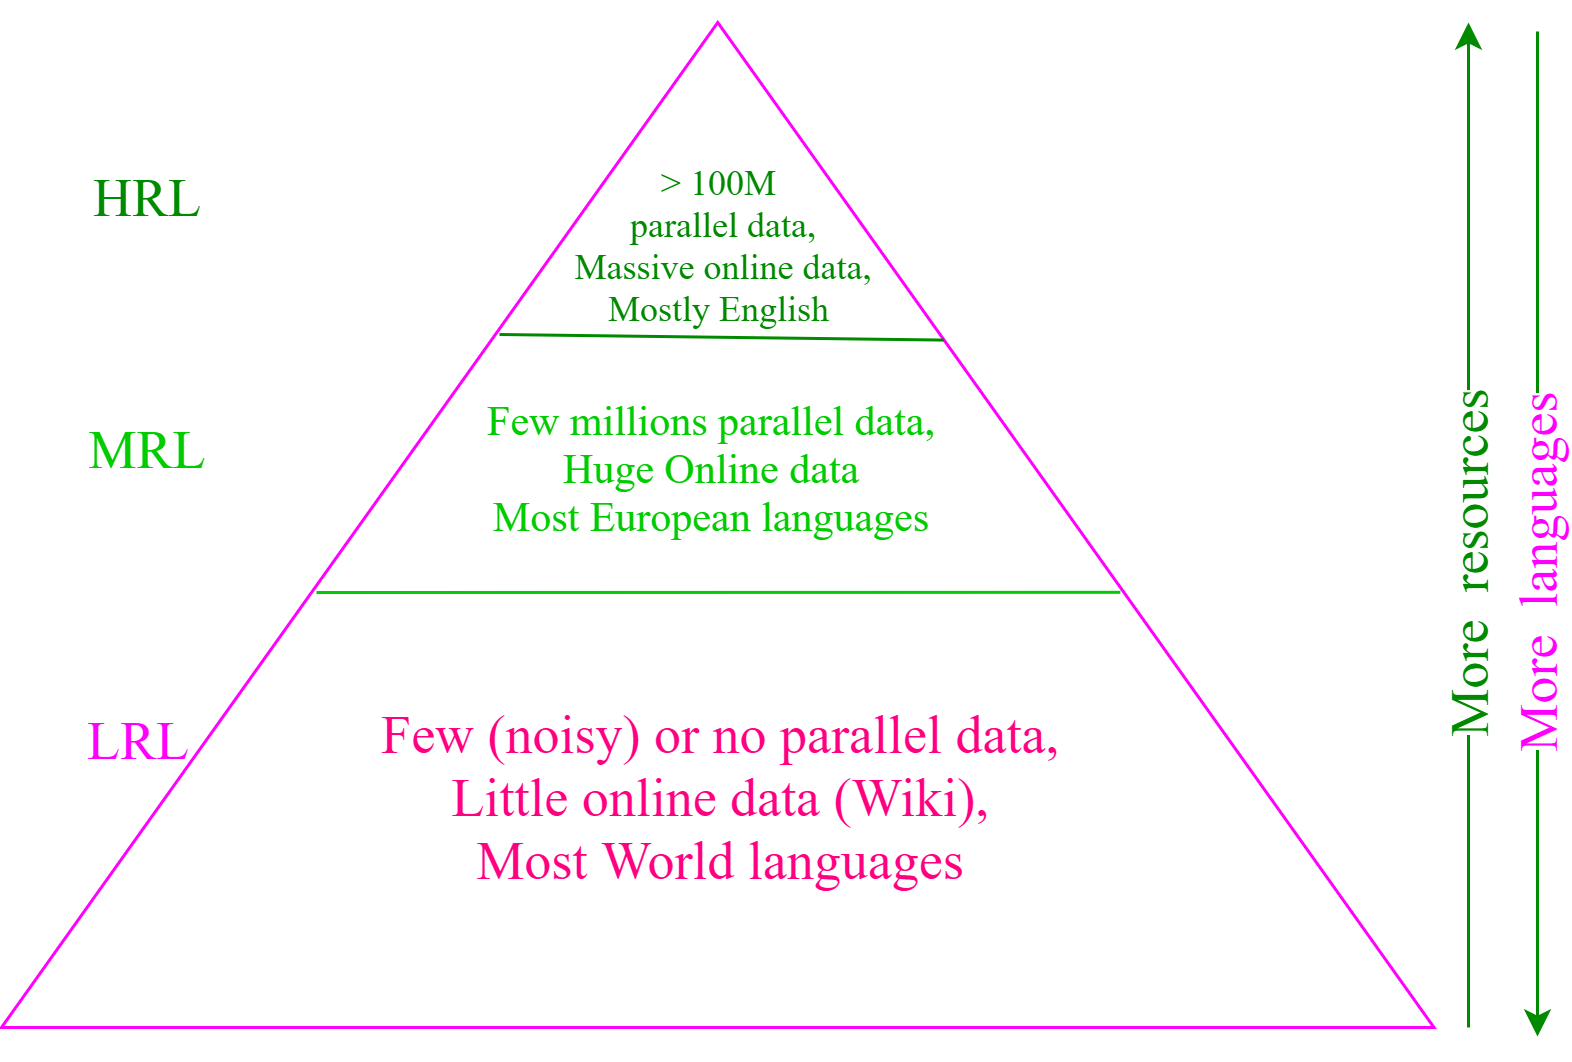
\includegraphics[width=0.7\linewidth]{resourcePyramid.png}
  \caption{Resource Pyramid}
  \Description{Resource Pyramid}
  \label{Resource-Pyramid}
\end{figure}

\textbf{Importance of Low Resource Language $\colon$}
Artificial Intelligence has significant success in human-like communication with computers by the most popular languages like English, Chinese, or other languages that have text corpora of hundreds of millions of words and other digital resources. Among 7,117 \footnote {\url{https://www.ethnologue.com/guides/how-many-languages}} human languages in the World, only a few (23 approx.) has been given proper care with digitalization.
However, the majority of languages remained to deprive of less computation work due to few or non-availability of large monolingual or parallel corpora and (or) sufficient handcrafted linguistic rules. These languages bereaved to perform more widespread benefits. It desperately needs tools and resources to overcome the resource barrier to NLP. As the minor or extinct languages are an indispensable part of the World language, so NLP application is the only means for ensuring communication between such languages.  
The selection criteria for low resource languages are highly specific to individual goals and context of a particular task. 
Because of an intrinsic characteristic of human conversations, an ambiguity of natural languages could be such as lexical, syntactic, semantic, pragmatic. \cite{cieri2016selection} explains the criteria applied to select languages for study within US programs that are included in low resource languages are as follows:
\begin{enumerate}
\item \textbf{Preservation of language --}
Most of the World’s languages will fall out of use before the World’s linguists and computational linguists are able to collect sufficient data~\cite{bird2012machine}. There is a race to save the World's disappearing languages. The main objective of the International mother language day (established in 1999), is to promote the preservation and protection of all languages used by peoples of the World. A language loses by humanity that loses the potential for greater diversity like cultural, intellectual, linguistic, oral traditions, etc.
\item \textbf{Community identity reclamation --}
Mother tongue must be the medium of instruction to preserve cultural diversity, and the heritage of a community. From the perspective of the communities, it gives new life to a language. Still, the revival and revitalization are arguably most important to keep the language away from the danger of extinct. The people for whom the language is being reclaimed, the reclamation of identity is of paramount importance. Hebrew was one of the languages revived from extinction with the help of NLP techniques.
\item \textbf{Commercial value --}
The language industry is a big business. The well-known machine translation systems (such as Google translate, Facebook, eBay, Microsoft, Systran translate, Babel Fish, KantanNMT) have extensive commercial use. According to the report \footnote { \url{https://www.gala-global.org/industry/industry-facts-and-data}}, the market will increase to US\$56.18 billion by 2021. The African continent has very high linguistic diversity, with an estimated one-third of the World’s 7,117 \citet{glottolog} languages from five major language families with 1.3 billion people. However, 1.4 billion people in India speak more than 19500 languages \footnote {\url{ https://gulfnews.com/world/asia/india/census-more-than-19500-languages-spoken-in-india-as-mother-tongues-1.2244791}}. The World online site depicts the statistics of the number of online users are increasing gradually.

\item \textbf{Knowledge augmentation --}
Most of the World's knowledge is not in text or corpora. The corpora do not contain what a speaker exactly explain by understanding a matter. Spoken language riddled with verbal disfluencies that interrupt the flow of speech, including long pauses, repeated words or phrases, restarts, and revisions of content. Human language is a system constructed to convey the speaker/writer's meaning. Different fast-growing collection of NLP techniques might found insight into a speaker/writer's understanding easily with more diverse languages.
\item \textbf{Social good reasons --}
As humanity extends our prevention by the emergency response, (an earthquake struck Haiti, where most local services failed, and all cell towers remained functional \footnote{ \url{http://web.stanford.edu/class/cs124/}}) identifying the outbreak of diseases saves other people's lives. In addition to helping companies process data, sentiment analysis also helps us understand society.
\item \textbf{Monitoring demographic and political processes --}
A minority language is a language spoken by a minority of the population of a territory usually hidden from World online active users. In Australia, a  small Island like South Goulburn, some 500 people speak around nine different languages. NLP can be helpful in this regard by developing an application of translation procedure. 
\end{enumerate}

This survey is organized as follows $\colon$  Section~\ref{motive} presents the motivation of our survey consisting of related work, survey gap, and scope of our review.  Section~\ref{contribute} presents the contribution of the survey. Section~\ref{method} presents the methodology of procuring the previous research articles for doing the survey. Section~\ref{data} presents the sources of low-resource MT corpora which is obtained by contacting the authors or organizers. Section~\ref{project} presents different projects held regarding low resource languages. Section~\ref{approach} presents an overall taxonomy of approaches towards the low-resource NMT system. 
Section~\ref{neural} discusses an integral part of the backbone of the current MT system, neural machine translation. 
Section~\ref{strategy} explains the different techniques and solution features of two approaches of low-resource NMT.  
Section~\ref{summarized} summarized in a tabular view of the surveyed techniques/solution features under the two approaches as traditional and knowledge transfer to low-resource neural machine translation that are the work-house for section~\ref{strategy}.
Section~\ref{discussion} discusses the future prospects and research avenue for the LR-NMT system. Finally, Section~\ref{conclusion} concludes our survey with a conclusion.

\section{Motivation of survey}
\label{motive}
In this section, we briefly review earlier studies related to our work. The low-resource Indian language translation poses the challenge of morphological and structural divergence of languages. The researchers have been working on low-resource NMT with the available limited corpora (\citet{philip2019baseline,choudhary2020neural, sen_hasanuzzaman_ekbal_bhattacharyya_way_2020,revanuru2017neural,ramesh2018neural,van2020optimal}). \citet{singhnmt} studied the techniques to alleviate low-resource scenarios of Indian language by word segmentation and pivot languages. \citet{singhimproving} presented a technique for low-resource Indian languages that uses linguistic features from rule-based feed to train neural machine translation systems.
The translation between Indo-Aryan languages is easier than that of the Dravidian language families, as earlier ones are less inflectional than later languages \citet{kunchukuttan2014sata}. Referring to this analysis on the SMT system, they have presented several different techniques to implement pivot based NMT and provide an overview of multilingual NMT. A survey on LR-NMT (\citet{liu2019survey}) introduced a variety of effective methods and models under low-resource conditions. The review elaborates on the existing problem and challenges of LR-NMT. 

A more detailed survey of methods to leverage monolingual data in LR-NMT, (\citet{gibadullin2019survey}) reviewed for improvement of low-resource language for NMT. This survey has presented some vital approaches, such as transfer learning, semi-supervised, and unsupervised learning techniques. Two ways of exploiting the monolingual data in the NMT system are architecture-dependent and independent. Architecture-independent methods include incorporating a language model with the encoder or decoder of the NMT system. Moreover, pre-training with the language model and multitasking under the architecture-dependent methods are designed for specific NMT models and may require significant modifications of their architecture. Further, these two methods are divided into broad categories that describe the improvements by achieving similarities and differences in their findings.

Another survey covered (\citet{yang2020survey}) several milestones in NMT. They investigated the principal development timeline of NMT, indicating the bottleneck in the development of SMT miniature towards the motivation of NMT. The study includes a variety of traditional seq-seq architecture to the variational transformer of NMT in the context of Deep learning. The survey discussed the training and inference methods of the variation of RNN over CNN and advanced models for NMT. Further, they argued that the multilingual translation process is the hot-spot for LR-NMT. \citet{alshemali2020improving}, discovered a comprehensive study using adversarial examples to enhance the reliability of DNN models in NLP. Most recently, \citet{dabre2019brief} reviewed multilingual neural machine translation about multiway, low or zero-resource (pivot-based, zero-shot and transfer learning approaches) and multi-source translation.

\textbf{The survey gap}
A very little survey work is available regarding low-resource language for NMT as per our concern. Most of the previous studies on low-resource Indian languages considered the statistical machine translation system. The researchers viewed that very few reviews on the research work related to low-resource language on NMT have been presented. Moreover, there is a minimal survey on exploring different underlying architecture on the LR-NMT system. Our study related to \citet{gibadullin2019survey}, where we studied several possible avenues but not limited approaches to LR-NMT. Our review focuses on several methods, techniques, solution features to effectively improve the capacity of NMT for low-resource problems. We investigated a lot about the relevant literature up-to-date trend and provided a comprehensive interpretation of current mainstream technology dedicated to LR-NMT only.

\textbf{The survey scope}
We have deliberately left out some of the approaches to NMT rather than using the terminology, such as domain adaptation in NMT, to embed NMT with other MT approaches (such as SMT, RBMT, HMT). Our study concerns the inclusion of techniques irrespective of considering more languages for LR-NMT. This review literature presents the studies that have done without considering the specific underlying architecture, resource tools associated with different approaches to LR-NMT. 

\section{Contribution of Survey}
\label{contribute}
This survey aims to enhance the performance of neural machine translation (NMT) in settings where parallel resources are limited or nil, for instance, to a small parallel corpus and (or) a bilingual lexicon. This survey interprets the limited or low resource, which is insufficient (little) for building an NLP application or having zero parallel sentences of translated languages. In a broader sense, this survey pursues two strategies that is data augmentation and knowledge transfer for improving the performance of LR-NMT. As per our knowledge, no prior survey work has been made explicit in considering different techniques of low-resource languages in NMT. The contribution of this article dwells in the following aspects:
\begin{enumerate}
    \item The survey is dedicated to explicitly low-resource NMT only.
    \item We investigate whether different data-augmentation processes help the NMT system for less-resourced language.
    \item This survey has shown prominent semi-supervised and unsupervised approaches compared to traditional supervised LR-NMT.
    \item We have explored a variety of transfer learning (multilingual NMT, Meta-learning) strategies to improve the performance of LR-NMT. 
    \item The review has presented a zero-resource translation approach as a pivot-based and zero-shot translation for low-resource language scenarios to the NMT system.
    \item We investigate whether synthetic data benefits the multi-modal machine translation system for less-resourced language.
    \item The study further reviews various types of defensive strategies through several research papers, explores current challenges for LR-NMT involving most of the techniques and highlights possible future research directions.
\end{enumerate}

To Bridge the gap, the survey is presented with tabular explanation through different techniques. We hope that our work could assist in further research.

\section{Survey Methodology}
\label{method}
To identify articles for this survey, we have explored Google, Google Scholar, Semantic Scholar, IEEE Xplore, ScienceDirect and ACL Anthology. Our query terms includes low-resource language, define: low-resource neural machine translation, low-resource OR resource-poor OR less-resourced Neural machine translation, recent approaches in low-resource language, recent approaches in low-resource neural machine translation, unsupervised low-resource language, unsupervised neural machine translation, demystifying techniques in low-resource language, universal NMT for low-resource language, data augmentation on low-resource neural machine translation, low resource Indian language processing, transfer learning on low-resource neural machine translation system, zero-shot translation in NMT, multi-modal neural machine translation, and meta-learning on low-resource language processing. Initially, for searching the articles, we used Google Scholar as a primary method. Google Scholar is potentially useful in systematic reviews of a specific topic of study. Google Scholar displays a list of different bibliographic databases filtered as required by pressing related articles. The papers shown are sorted further as per relevance by clicking ``Sort by relevance''. Then we have selected the articles by setting the time limit to 2020 in Google Scholar. In our survey, the related papers on low-resource neural machine translation are included, excluding those that do not contain both the phrases ``low-resource'' and ``neural machine translation''. If such relevant articles are unavailable, then other alternatives are explored until we find similar papers. While searching for the above queries in a broader sense in Google Scholar, it displayed relevant articles (default 10) in several pages, out of which only two pages were considered. From the selected two pages, we have chosen 3 to 5 relevant articles that match our queries. We have referred to a total of 229 papers in this survey, out of which 96 articles are kernel to the low-resource neural machine translation that are summarized in a tabular view. Some papers are searched directly through the Journal by taking the article name from the reference list of a relevant document. We have also explored the homepage of researchers' who had contributed to NMT regarding LRL. Several techniques or methods implemented by researchers of NMT-community, especially low-resource language on data augmentation and knowledge transfer has also reviewed. Finally, current research papers (till 2020 June), recent blogs such as Facebook AI, Google AI, Microsoft Research, as well as workshops, conferences of low-resource language have reviewed for conducting this systematic survey. 

\section{Source of low resource dataset}
\label{data}
The parallel corpus is one of the most valuable resources for many multilingual NLP applications, especially machine translation. Parallel corpora play a crucial role in neural machine translation. Many approaches have been proposed to obtain bilingual corpus automatically (\citet{zhu2019novel}). Effective Machine Translation (MT) requires massive amounts of training data to produce intelligible results. Several workshops (WAT [16-17,19-20]), AfricaNLP Workshop, shared tasks (WMT[18-20]) and proposals (Facebook research) on low-resource MT have been organized for various languages from time to time. To this date, Wikipedia is one of the most useful resources as a knowledge base for training ML methods, low-resource machine translation, entity linking and disambiguation, language modeling, other variety of other tasks. OPUS \footnote{\url{http://opus.nlpl.eu/}} is an augmenting collection of translated sentences from the web to provide the community with a publicly available parallel corpus. Websites are crawled to collect parallel sentences for processing NMT systems. ParaCrawl \footnote{\url{https://paracrawl.eu/}} project provides parallel corpora for European Languages. Parallel corpora are available from various providers by freely accessible or built with proprietary data. Primary language parallel translation corpus are English-Hindi \footnote{\url{http://www.cfilt.iitb.ac.in/iitb\_parallel/}}, PMIndia corpus \footnote{\url{http://data.statmt.org/pmindia/}}, Indian Languages Corpora Initiative (ILCI) \footnote{\url{http://sanskrit.jnu.ac.in/ilci/index.jsp}}, WAT 2018 parallel corpus for a multilingual task \footnote{\url{ http://lotus.kuee.kyoto-u.ac.jp/WAT/indic-Multilingual/index.html}}, 
Charles University parallel corpus \footnote{For English-Hindi: \url{ https://lindat.mff.cuni.cz/repository/xmlui/handle/11858/00-097C-0000-0001-BD17-1}, English-Tamil: \url{ttps://lindat.mff.cuni.cz/repository/xmlui/handle/11234/1-2879}, English-Odia:  \url{https://lindat.mff.cuni.cz/repository/xmlui/handle/11234/1-2879}, and English-Urdu:  \url{https://lindat.mff.cuni.cz/repository/xmlui/handle/11234/1-2582}}, IndoWordnet Parallel corpus \footnote{\url{https://github.com/anoopkunchukuttan/indowordnet_parallel}}, Parallel corpora for 6 Indian languages created on Mechanical Turk \footnote{\url{https://github.com/joshua-decoder/indian-parallel-corpora}}, TED-Multilingual-Parallel-Corpus \footnote{\url{https://github.com/ajinkyakulkarni14/TED-Multilingual-Parallel-Corpus}}, JW300 parallel corpus for low-resource languages \footnote{\url{http://opus.nlpl.eu/JW300.php}}, Asian Language Treebank Parallel Corpus (13 languages) \footnote{\url{http://www2.nict.go.jp/astrec-att/member/mutiyama/ALT/}}, 
Facebook Low Resource MT Benchmark (FLoRes) \footnote{\url{ https://github.com/facebookresearch/flores}}, Uka Tarsadia University English-Gujarati parallel corpus \footnote{\url{ https://github.com/shahparth123/eng\_guj\_parallel\_corpus}}, NLPC-UoM English-Tamil Corpus \footnote{\url{ https://github.com/nlpc-uom/English-Tamil-Parallel-Corpus}}, 
Bhojpuri Language Technological Resources (BHLTR) 
\footnote{\url{https://github.com/shashwatup9k/bho-resources}}, English to Indian Language Machine Translation (EILMT) consortium \footnote{\url{http://tdil-dc.in/index.php?searchword=EILMT&searchphrase=all&option=com_search&lang=en}}, 
WikiMatrix \footnote{\url{https://github.com/facebookresearch/LASER/tree/master/tasks/WikiMatrix}}: bitext extraction of 135 million Wikipedia sentences in 1,620 language pairs, CCMatrix \footnote{\url{https://github.com/facebookresearch/LASER/tree/master/tasks/CCMatrix}}: extracting billions of high-quality parallel texts on the WEB, large monolingual corpora (IndicNLP corpus) \footnote{\url{https://github.com/ai4bharat-indicnlp/indicnlp\_corpus}}. Urdu-Nepali-English parallel corpus  \footnote{\url{http://www.cle.org.pk/software/ling\_resources/UrduNepaliEnglishParallelCorpus.htm}}, A huge amount of parallel corpus: the Bible in 100 languages \footnote{\url{https://github.com/christos-c/bible-corpus}}, United Nations parallel corpus \footnote{\url{https://conferences.unite.un.org/UNCorpus/}}, Wikimedia \footnote{\url{https://dumps.wikimedia.org/}}, European Parliament Proceedings Parallel Corpus 1996-2011 \footnote{\url{http://www.statmt.org/europarl/}}, Korean parallel corpora \footnote{\url{https://github.com/jungyeul/korean-parallel-corpora}}, SDL offers commercial customers to deliver trained language pairs that leverage neural machine translation \footnote{\url{https://www.sdl.com/software-and-services/translation-software/machine-translation/language-pairs.html}}, Autshumato parallel corpora \footnote{For English-Setswana :\url{https://repo.sadilar.org/handle/20.500.12185/404}, English-isiXhosa \url{https://repo.sadilar.org/handle/20.500.12185/525} and Monolingual-isiXhosa \url{https://repo.sadilar.org/handle/20.500.12185/524}}, Tatoeba multilingual large database of sentences and translations \footnote{\url{https://tatoeba.org/eng/stats/sentences_by_language}{Tatoeba}}, European Union open data \footnote{\url{https://data.europa.eu/euodp/en/data}}, and DGT-EC (European Commission) \footnote{\url{https://ec.europa.eu/jrc/en/language-technologies/dgt-translation-memory}}. Some of the datasets mentioned here can be obtained by contacting the authors or organizations. Other corpora used by researchers in LR-NMT are stated in the summary table of their article.

\section{Low-resource language projects for machine translation}
\label{project}
There is rising attention for the improvement of low-resource/low-density languages internationally by a growing number of programs supported by government, non-government, linguistic organizations, and indigenous communities. The United States sponsored and organized several intensively multilingual programs with multiple technologies, have focused on developing language resources and techniques of low-resource languages. The programs are the DARPA TIDES (Translingual Information Detection, Extraction, and Summarization), REFLEX (Research on English and Foreign Language Exploitation) LCTL program, National Institute of Standards and Technologies (NIST) Language REcognition (LRE) \footnote {\url{https://www.nist.gov/itl/iad/mig/language-recognition}}, IARPA Babel \footnote {\url{ https://www.iarpa.gov/index.php/research-programs/babel}}, DARPA LORELEI \footnote {\url{  http://www.darpa.mil/program/low-resource-languages-for-emergent-incidents}}, and the Digital Language Diversity Project (DLDP) \footnote{ \url{http://www.dldp.eu/en/content/project}}. 

\section{Approaches to low-resource NMT system}
\label{approach}
% Those papers not included in the table, referred as a related study. 

Parallel corpora are usually limited in quantity, quality, and coverage, especially for low-resource languages. Previously NMT focused on large vocabularies (\citet{jean2015using,mi2016vocabulary}), better techniques for handling unknown words (\citet{luong-etal-2015-addressing,sennrich2016neural,li2016towards}), creating better alignment mechanisms for the encoder-decoder network (\citet{cheng2016neural,luong2015effective, cohn-etal-2016-incorporating,FENG18.3,tu2016modeling,mi2016coverage,mi2016supervised}) and improved objective functions for BLEU score (\citet{shen2016minimum}). \citet{ueffing2006using,wu2008domain} investigates using self-learning algorithms in the conventional SMT system of source-side monolingual data.
NMT for low-resource languages represents a challenge \citet{koehn2017six}. The data-hungry NMT system does not operate well in low-resource languages (\citet{zoph2016transfer,ostling2017neural}). 
However, low resource languages that lack sufficient parallel datasets face challenges in the automated translation filed. Several efforts have shown to improve translation performance in low-resource settings. The question arises as to why the usual techniques used in NLP could not be applied to these low-resource languages. The apparent reason is that the requirement of expertise handcrafted rules in the rule-based system is time-consuming and expensive. On the other hand, a large amount of data is required to learn parameters for SMT systems.

Two main approaches for handling the problem in the low-resource setting, where the amount of data and the knowledge of the language are insufficient and have fewer technologies: 
\begin{enumerate}
    \item Traditional approach
    \item Knowledge transfer approach
\end{enumerate}
\textbf{Traditional approach $\colon$}
Statistical Machine Translation (SMT) sounds much more fluent compared to Rule-based Machine Translation (RBMT). These two approaches have been dominant over the past years. In the research literature, these methods are considered as the traditional approach. Recently, NMT has made significant progress in high resource and medium resource language pairs.    
The traditional (not that word used customarily) approach of low-resource language focuses on leveraging labeled data for a single language or a variety of languages through active learning (can ask speakers) or using different techniques from massive available monolingual data. In the translation process, the holistic neural network used as a model based on encoder-decoder in the NMT system. The end-to-end training makes NMT excel over conventional SMT significantly on the system's performance. However, the NMT systems based on \citet{sutskever2014sequence, DBLP:journals/corr/BahdanauCB14,luong2015effective,vaswani2017attention} underperform on unsupervised methods in low-resource data conditions (\citet{sennrich2019revisiting}). Hybridizing the RNN and CNN  architecture, the character neural machine translation model an effective way of translating two low-resource languages (\citet{almansor2018hybrid}). Researchers have been applying several approaches for processing low-resource languages (LRLs) in NMT system. Handling rare words, several data augmentation methods such as back translation, using monolingual corpora, cross-lingual word embedding, language model fusion are considered as a traditional approach for processing the low-resource neural machine translation system.\\
\textbf{Knowledge transfer approach $\colon$}
Transferring knowledge from a high-resource source language to a low-resource target language is known as transfer learning. To increase the performance of the target learning task, the knowledge from the source task and source domain transferred, where the size of the source domain is much larger than the target domain (refer figure~\ref{RecLRL}). Transfer learning, multitasking, multilingual, zero-resource translation, and meta-learning are considered as knowledge transfer approach for processing the low-resource neural machine translation system. 

\begin{figure}[!h]
  \centering
  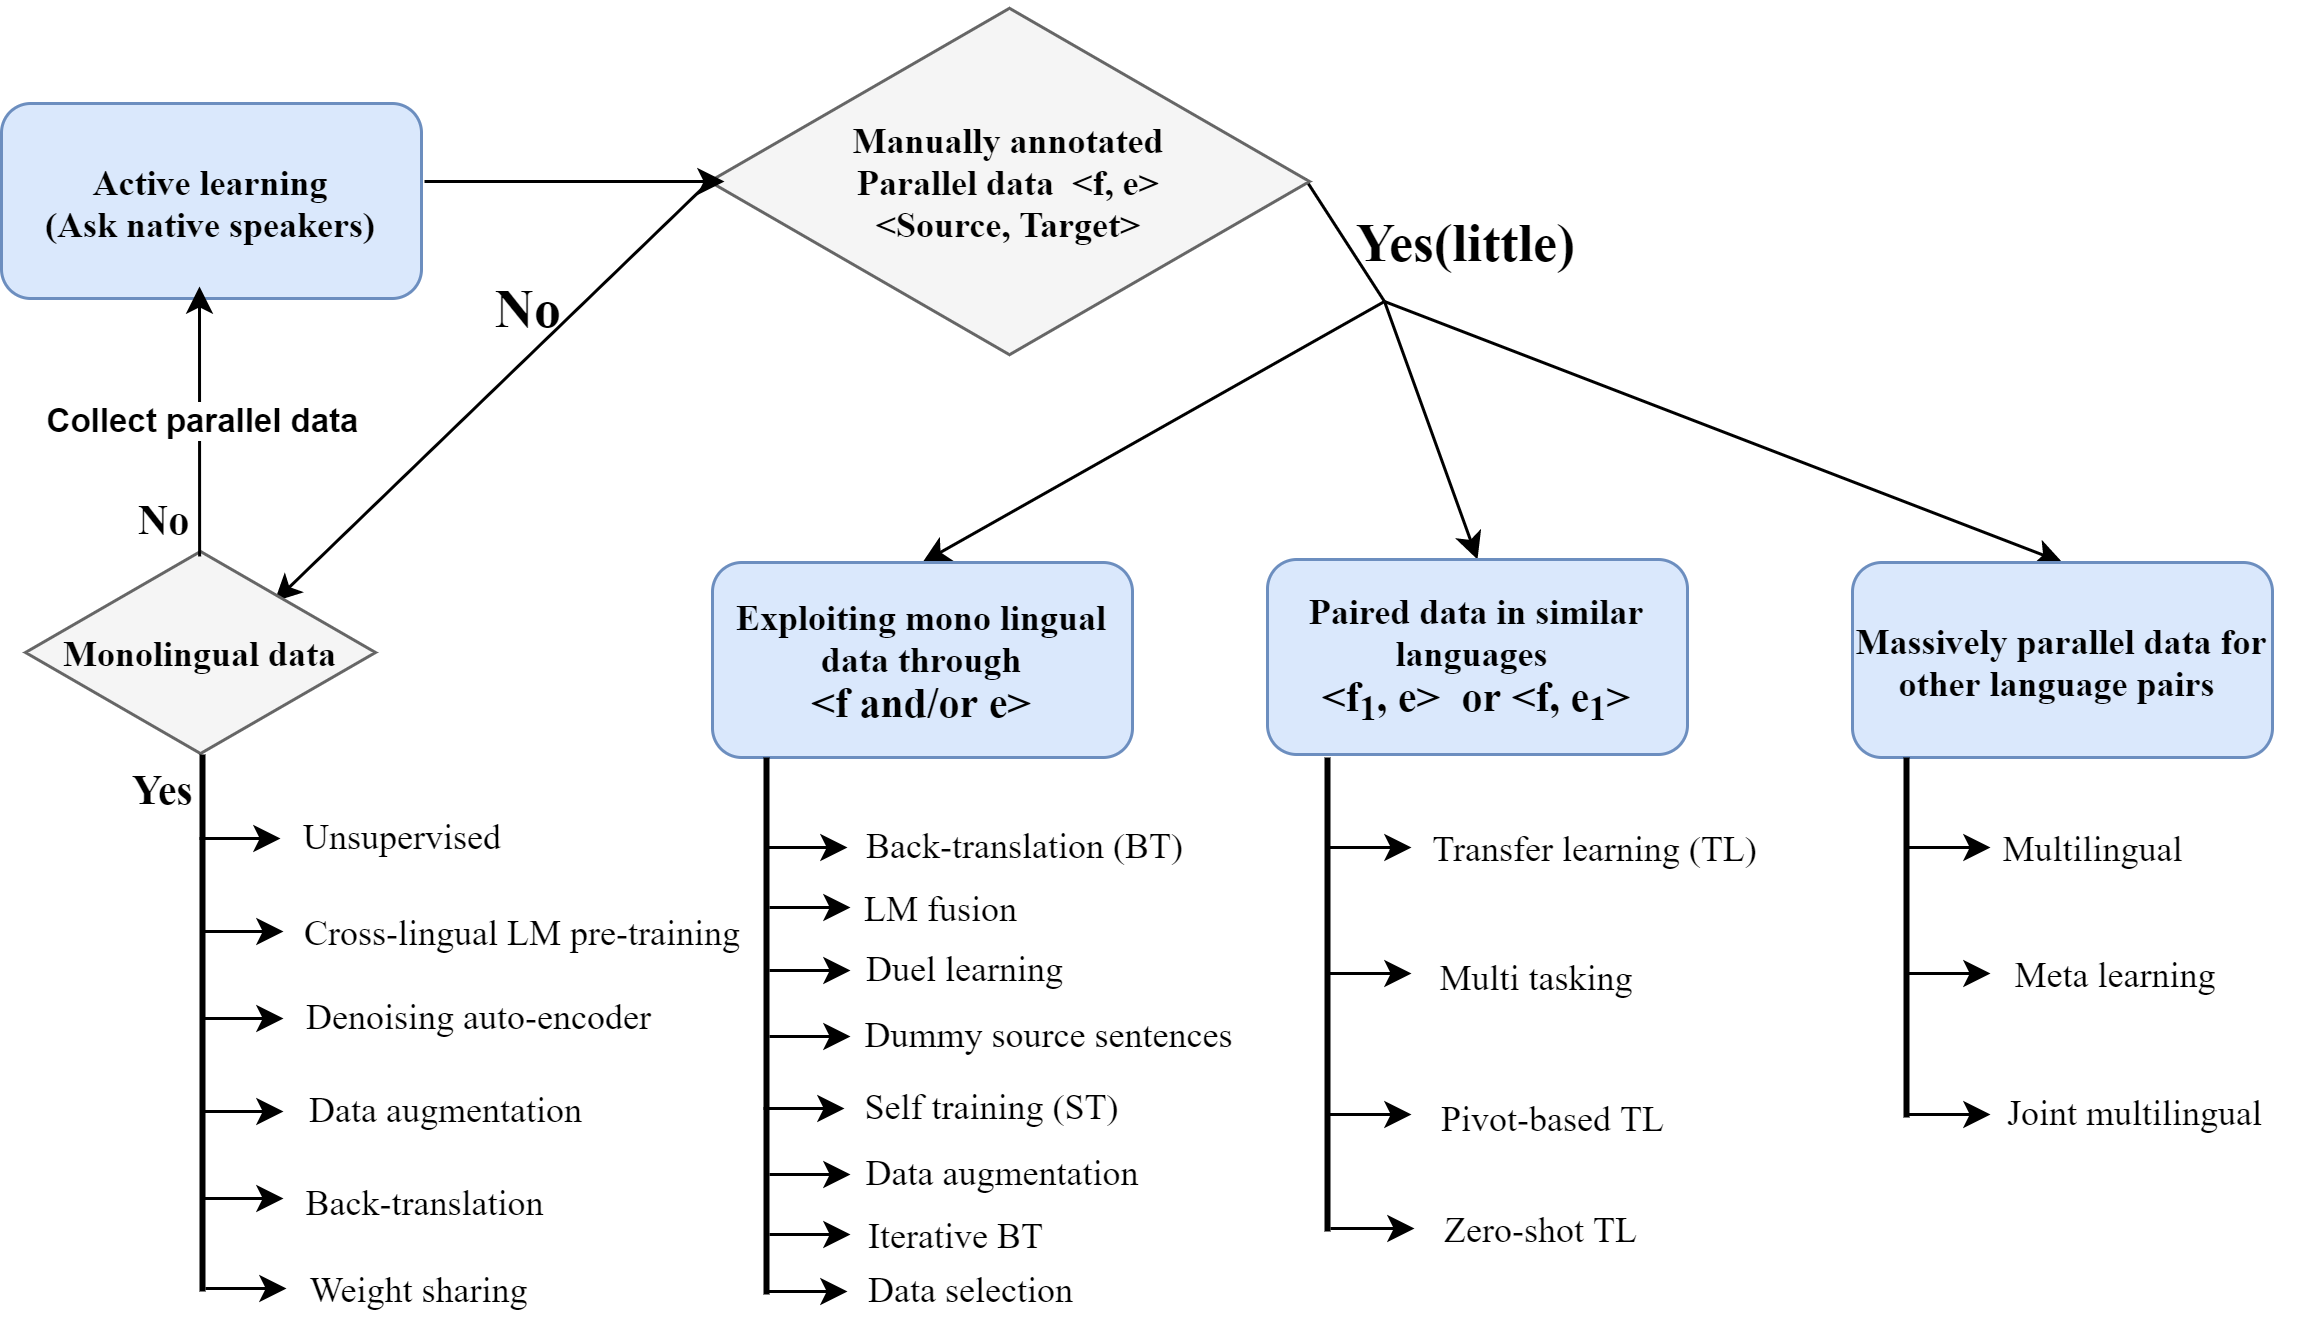
\includegraphics[width=0.9\linewidth]{LRLRecipe.png}
  \caption{Low-resource language recipe}
  \Description{Recipe of Low-resource Language }
  \label{RecLRL}
\end{figure}



\section{Neural Machine translation}
\label{neural}
Machine Translation is a classic test of language understanding that consists of both language analysis and generation.
Notwithstanding the massive success brought by NMT (\citet{sutskever2014sequence,DBLP:journals/corr/BahdanauCB14,bojar2016findings}), WIPO (\citet{pouliquen2017wipo, vaswani2017attention}), Google (\citet{wu2016google}) and Systran (\citet{crego2016systran}), there have also been reports of the poor performance of NMT often lags behind the conventional MT systems, for low-resource language pairs in statistical phrase-based translation systems (PBMT) (\citet{koehn2003statistical}). 
\citet{koehn2017six} describes the challenges of NMT systems that have better performance in high-resource settings and worse quality in low-resource scenarios. 
However, it is known that both vanilla NMT and SMT shows poor performance for low resource scenarios of the domain-specific corpus
 (\citet{duh2013adaptation,sennrich2013multi,zoph2016transfer,koehn2017neural}).

A major development in SMT is the adoption of neural networks \cite{koehn2017neural}. NMT is aiming at end-to-end machine translation without phrase table extraction and language model training.
NMT approach uses sequence-to-sequence transduction using deep semantic representations of the source text. The NMT investigates various methods to formalize attention mechanisms and decoding over structures such as graphs, trees, lattices, and forests. This formalization can be used in the encoder-decoder architecture to generate the output while attending various parts of the input. \textbf{Why welcome NMT?} LSTM with attention network can take into account the entire context of the source sentence generated so far and create more accurate and fluent translations. It solves the difficulty of translating between languages with notably different word orderings. Generating placeholder for unknown words, the soft-alignment of the NMT module passes the exact source word to the target sentence. A vocabulary reduction technique by combining the most frequently occurring words in the target vocabulary can reduce the size of the output layer of the NMT module. Without degrading the quality, it helps to make computation faster. Fine-tuning an optimal set of hyperparameters such as learning rate, attention type, number of epochs, have a significant impact on different models of each translation direction. The NMT, which models direct mapping between source and target languages, has achieved a significant breakthrough in translation performance. The word embeddings approach makes NMT possible to measure the semantic similarity between words.

The NMT system considers an entire sentence of parallel data contrary to SMT's n-gram language model. The sequence of words is quite fluent in phrase wise, whereas overall sentences might not be fluent in the SMT system. The LSTM RNN can efficiently handle the long-distance dependencies that make NMT systems tends to be a lot more fluent than the output of SMT systems. In NMT, several components are jointly trained to a single complex model as compared to independently learned different modules of SMT. The single model can capture inter-dependencies between the complex features of languages. The conference of SlatorCon Zurich reveals that NMT lessens post-editing effort by 25\% outputs and is more fluent in translations than SMT. According to a language technology developer, particularly for smaller European languages, Tilde revealed that the NMT system control (1) word ordering and (2) morphology, syntax and agreements (considering long-distance) up to five and three times better, respectively, than the SMT system. Noise in the training corpus is more sensitive towards results than the SMT system. Word-based NMT with attention is far superior to word-based SMT. Translating between multiple languages and zero-shot translations are easily possible with NMT for low-resource languages.
The strength and weaknesses of NMT and detailed analysis of NMT versus SMT explored by (\citet{bentivogli2016neural,isabelle2017challenge,koehn2017six,mahata2018smt}) are the challenges of NMT compared with its previous approach to machine translation.
Several state-of-the-art NMT architectures can significantly outperform existing SMT architectures for the translation of low-resource languages (\citet{abbott2018towards, martinus2019focus}). In most cases, replacing PB-SMT with NMT seems to incur no quality loss in BLEU (\citet{junczys2016neural}).

\section{Strategies of neural machine translation for low-resource language}
\label{strategy}
This section explains some unavoidable and crucial workhouse strategies of low-resource neural machine translation.
\subsection{Unsupervised Neural Machine Translation (UNMT)}
After statistical decipherment about unsupervised learning, in 2018, NLP gained exceptional ground in unsupervised-NMT. Training an MT model without access to human-made translation pairs with bilingual data at training time is called unsupervised translation. A complete UNMT rely on monolingual corpora only. The word embeddings for the target and source language are trained on the two monolingual corpora separately. An Unsupervised method ranks the translation of words by using a bilingual dictionary and wordnet. They acquire a linear transformation to correlate them to a latent space through adversarial or self-learning. The sub-word embeddings used to initialize a lookup table in the encoder and decoder of the UNMT system. Recently, some steps applied to build an UNMT by initializing shared encoder with shared cross-lingual BPE encoding, language modeling, and back-translation (BT) (on-the-fly). Language modeling accomplished via denoising autoencoding in NMT learns to reconstruct a sentence in a given language from a noisy version of it (\citet{xu2020spanish}). The BT and auto-encoding are critical components of UNMT. There is limited work with the NMT system in an entirely unsupervised manner. UNMT further improved through bootstrapping with unsupervised PBSMT is called NMT hybridization. A type of hybridization approach to UNMT in the figure~\ref{nmt-hybridization} shows an unsupervised SMT to warm up a dual NMT model trained through iterative back-translation (IBT). Initially, train two SMT systems in opposite directions to assist the training of another two NMT systems in opposite directions. The BT builds a synthetic parallel corpus in the SMT system in the opposite direction. Whereas in reverse NMT model, it progressively switches to a synthetic parallel corpus.

\begin{figure}[!h]
  \centering
  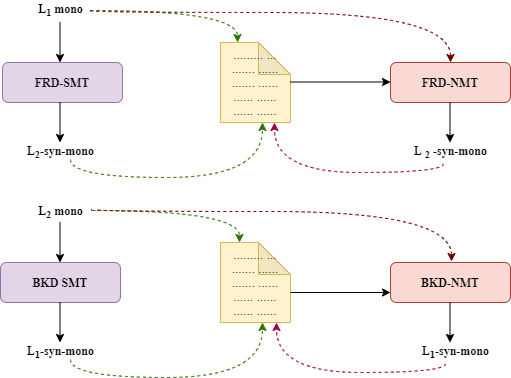
\includegraphics[width=0.5\linewidth]{NMTHybridization.png}
  \caption{NMT Hybridization}
  \label{nmt-hybridization}
\end{figure}

\subsection{Back-Translation (BT)}
BT operates in a semi-supervised setup using both bilingual and monolingual data of the target (and/or source) languages available. BT (refer figure~\ref{back-trans-and-iter-back-trans}) first trains an auxiliary translation system from the target language to the source language (reverse system), using the available parallel data. The auxiliary system translates the monolingual target data into the source language. The result is a parallel corpus where the source side is synthetic machine-translation output, while the target is an original text written by humans. The number of training data from the source language to target language has increased by simply adding the synthetic parallel corpus to the real bitext (real $+$ synthetic). The augmented training data is applied to train the final system to translate from the source to the target language. BT is an alternative to leverage monolingual data. The generation of parallel data through backward and forward directions with BT is used to build a better translation system. Taking the idea of BT one step further turns it into re-back-translate monolingual data for improving performance over BT under low-resource conditions. This process can be ``iterated'' several times and is called \textbf{Iterative Back-Translation (IBT)}. In IBT, two models can be used in both translation directions to train each other. The following figure \ref{back-trans-and-iter-back-trans} presents the re-back-translation process (repeated back-translation). 

\begin{figure}[!h]
\begin{minipage}{0.4\textwidth}
         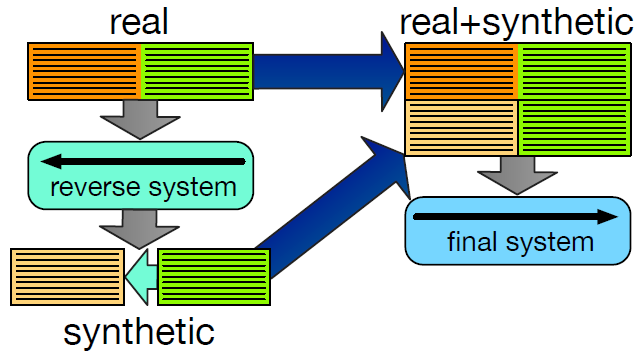
\includegraphics[width=0.8\linewidth]{backTranslationHoang2018.png} 
        % \caption{Back-translation}
        \label{back-trans}
\end{minipage}
\begin{minipage}{0.5\textwidth}
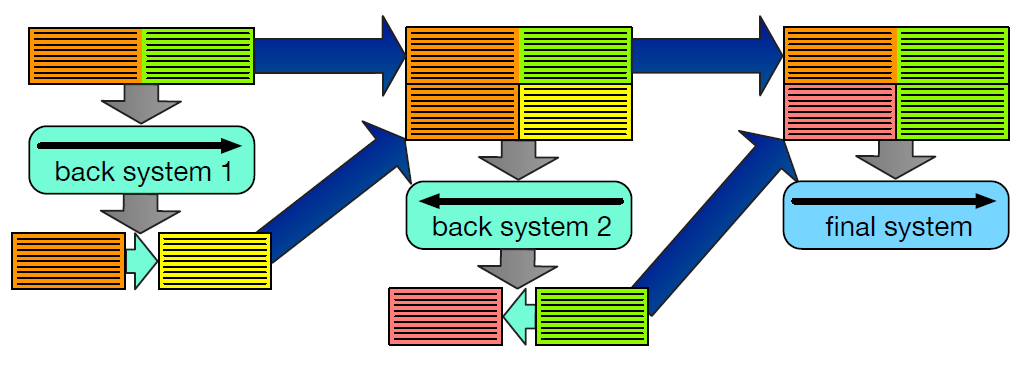
\includegraphics[width=0.9\linewidth] {IBT.png}
        % \caption{Iterative-back-translation}
\label{iter-back-trans}
\end{minipage}
        \caption{Back-translation and Iterative back-translation (referred from \citet{hoang2018iterative})}
        \label{back-trans-and-iter-back-trans}
\end{figure}


\begin{figure}[!h]
    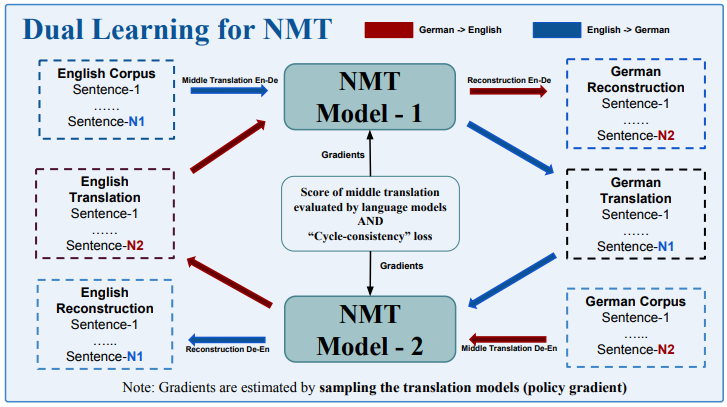
\includegraphics[width=0.9\linewidth]{duelLearningWangZhu.png} 
    \caption{Duel learning}
    \label{duel-learning}
\end{figure}

A more refined idea of BT is where it integrates the training on monolingual and parallel data via round-tripping known as \textbf{Duel learning} (\citet{he2016dual}) (refer figure \ref{duel-learning}) \footnote{The duel learning figure referred from Wang Zhu's homepage \url{https://billzhu.me/}}. Here, two agents participate in translating in opposite directions and teaching each other through reinforcement learning. The idea is to learn two language models from source and target languages with the monolingual data. This process serves to collect two kinds of reward signals $\colon$ ``language model reward'', measuring the fluency of the generated sentences, and ``communication reward'', assessing the quality of the machine translation system. The reverse model backpropagated through the model gradients. Duel learning mechanism enables an NMT system to learn from unlabeled data automatically. Duel learning mechanism can leverage both the source and target monolingual data effectively. 

\subsection{Shallow and deep fusion}
Another strategy for leveraging an ample amount of monolingual data is that integrate a language model (LM) trained on target monolingual data into an LR-NMT system. Conventionally, shallow fusion where monolingual LM incorporated into a decoder of SMT. At each time step, the Translation Model (TM) proposes a set of candidate words. The candidate score according to the weighted sum of scores given by LM and TM. Deep fusion integrates the RNNLM (language model implemented with RNN) and decoders of NMT concatenating their hidden states (refer figure \ref{shallow-deep-fusion}).

\begin{figure}[!h]
  \centering
  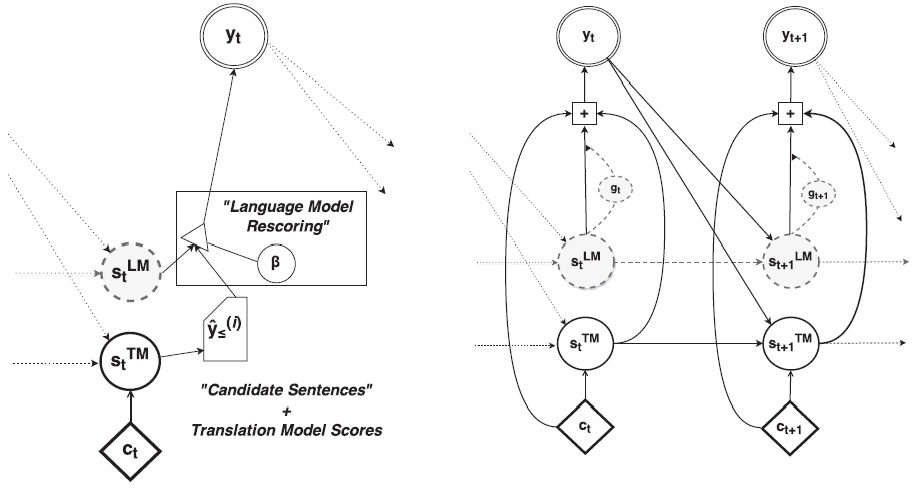
\includegraphics[width=0.8\linewidth]{shallowDeepFusionGulcehre.png}
  \caption{Shallow and Deep fusion (referred from \citet{gulcehre2017integrating})}
  \Description{shallow-deep-fusion}
  \label{shallow-deep-fusion}
\end{figure}

\subsection{Transfer learning}
Transfer learning (TL), initializes the parameters of the previously trained parent model ($E_s$-$F_t$ model: $E_s$-$F_t$ being the high-resource language pair where $E_s$ and $F_t$ are a source and target language respectively) to child model ($Z_s$-$F_t$ model: $Z_s$-$F_t$ being the low-resource language pair where $Z_s$ is source language). In this method, the target language ($F_t$) possesses the same vocabulary for both the parent and the child models. Based on domain and task, there can be many variations tackled using transfer learning in natural language processing, domain adaptation, cross-lingual learning, multi-task learning, and sequential transfer learning \citet{ruder2019transfer}. A parent (source) model trained on a large corpus, and then the weights of the hidden layers are transferred to a smaller target dataset and re-trained for a similar or different task. By taking the advantages of the source model, we find words that are syntactically and semantically similar to the target (child) model. The TL attempts to improve the performance on a new task using knowledge, depicted in figure~\ref{TLfigure}, obtained from the high-resource parent model of different tasks. An efficient technique for the NMT system under low-resource conditions is transfer learning.

\begin{figure}[!h]
  \centering
  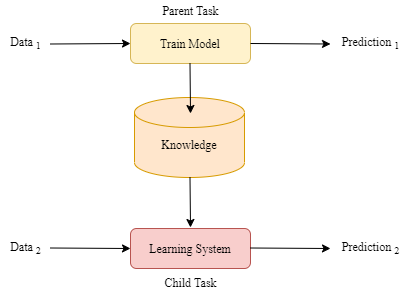
\includegraphics[width=0.5\linewidth]{TransferLearning.png}
  \caption{Learning process of Transfer Learning}
  \Description{Learning process of Transfer learning}
  \label{TLfigure}
\end{figure}

Transfer learning contributes to building accurate models in a time-saving way (\citet{rawat2017deep}). \citet{torrey2010transfer} explains three methods for improving the performance of transfer learning that are as follows:
\begin{enumerate}
    \item Enhancing the training performance at the initial state compared to a randomly initialized model during a similar task;
    \item Maximum performance obtained within a short period;
    \item Instead of training the model increasing the level of final performance without the transfer.
\end{enumerate}

\subsection{Self-training}
A semi-supervised approach that utilizes unannotated data to create better models is known as Self-training. In this strategy, an auxiliary model trained with little parallel data acts as a ``parent model'' to label the unannotated data, which is used to augment the original small training set. A ``child model'' is trained with this new training set to create the final model (refer figure \ref{self-training}). The goal is to augment more bilingual data using available small bilingual data and leverage enough source-side monolingual data. Self-training can work with unsupervised training and pseudo-supervised training as well. The noisy self-training could improve supervised machine translation performance, and synthetic data could play a decisive role, even as a target. The self-training mechanism used to generate synthetic training data for Unsupervised-NMT (UNMT) strategies to train a robust UNMT system to build a more desirable model. The self-training model learns the decoding process, and an injection of noise in the source sentence helps to generate similar inputs to the corresponding target. This way, the model learns to map the semantically similar sentences into the same target sentence. In low-resource translation, data are often out-of-domain. The self-training is a viable option to generate in-domain through source monolingual data.

\begin{figure}[!h]
    \centering
    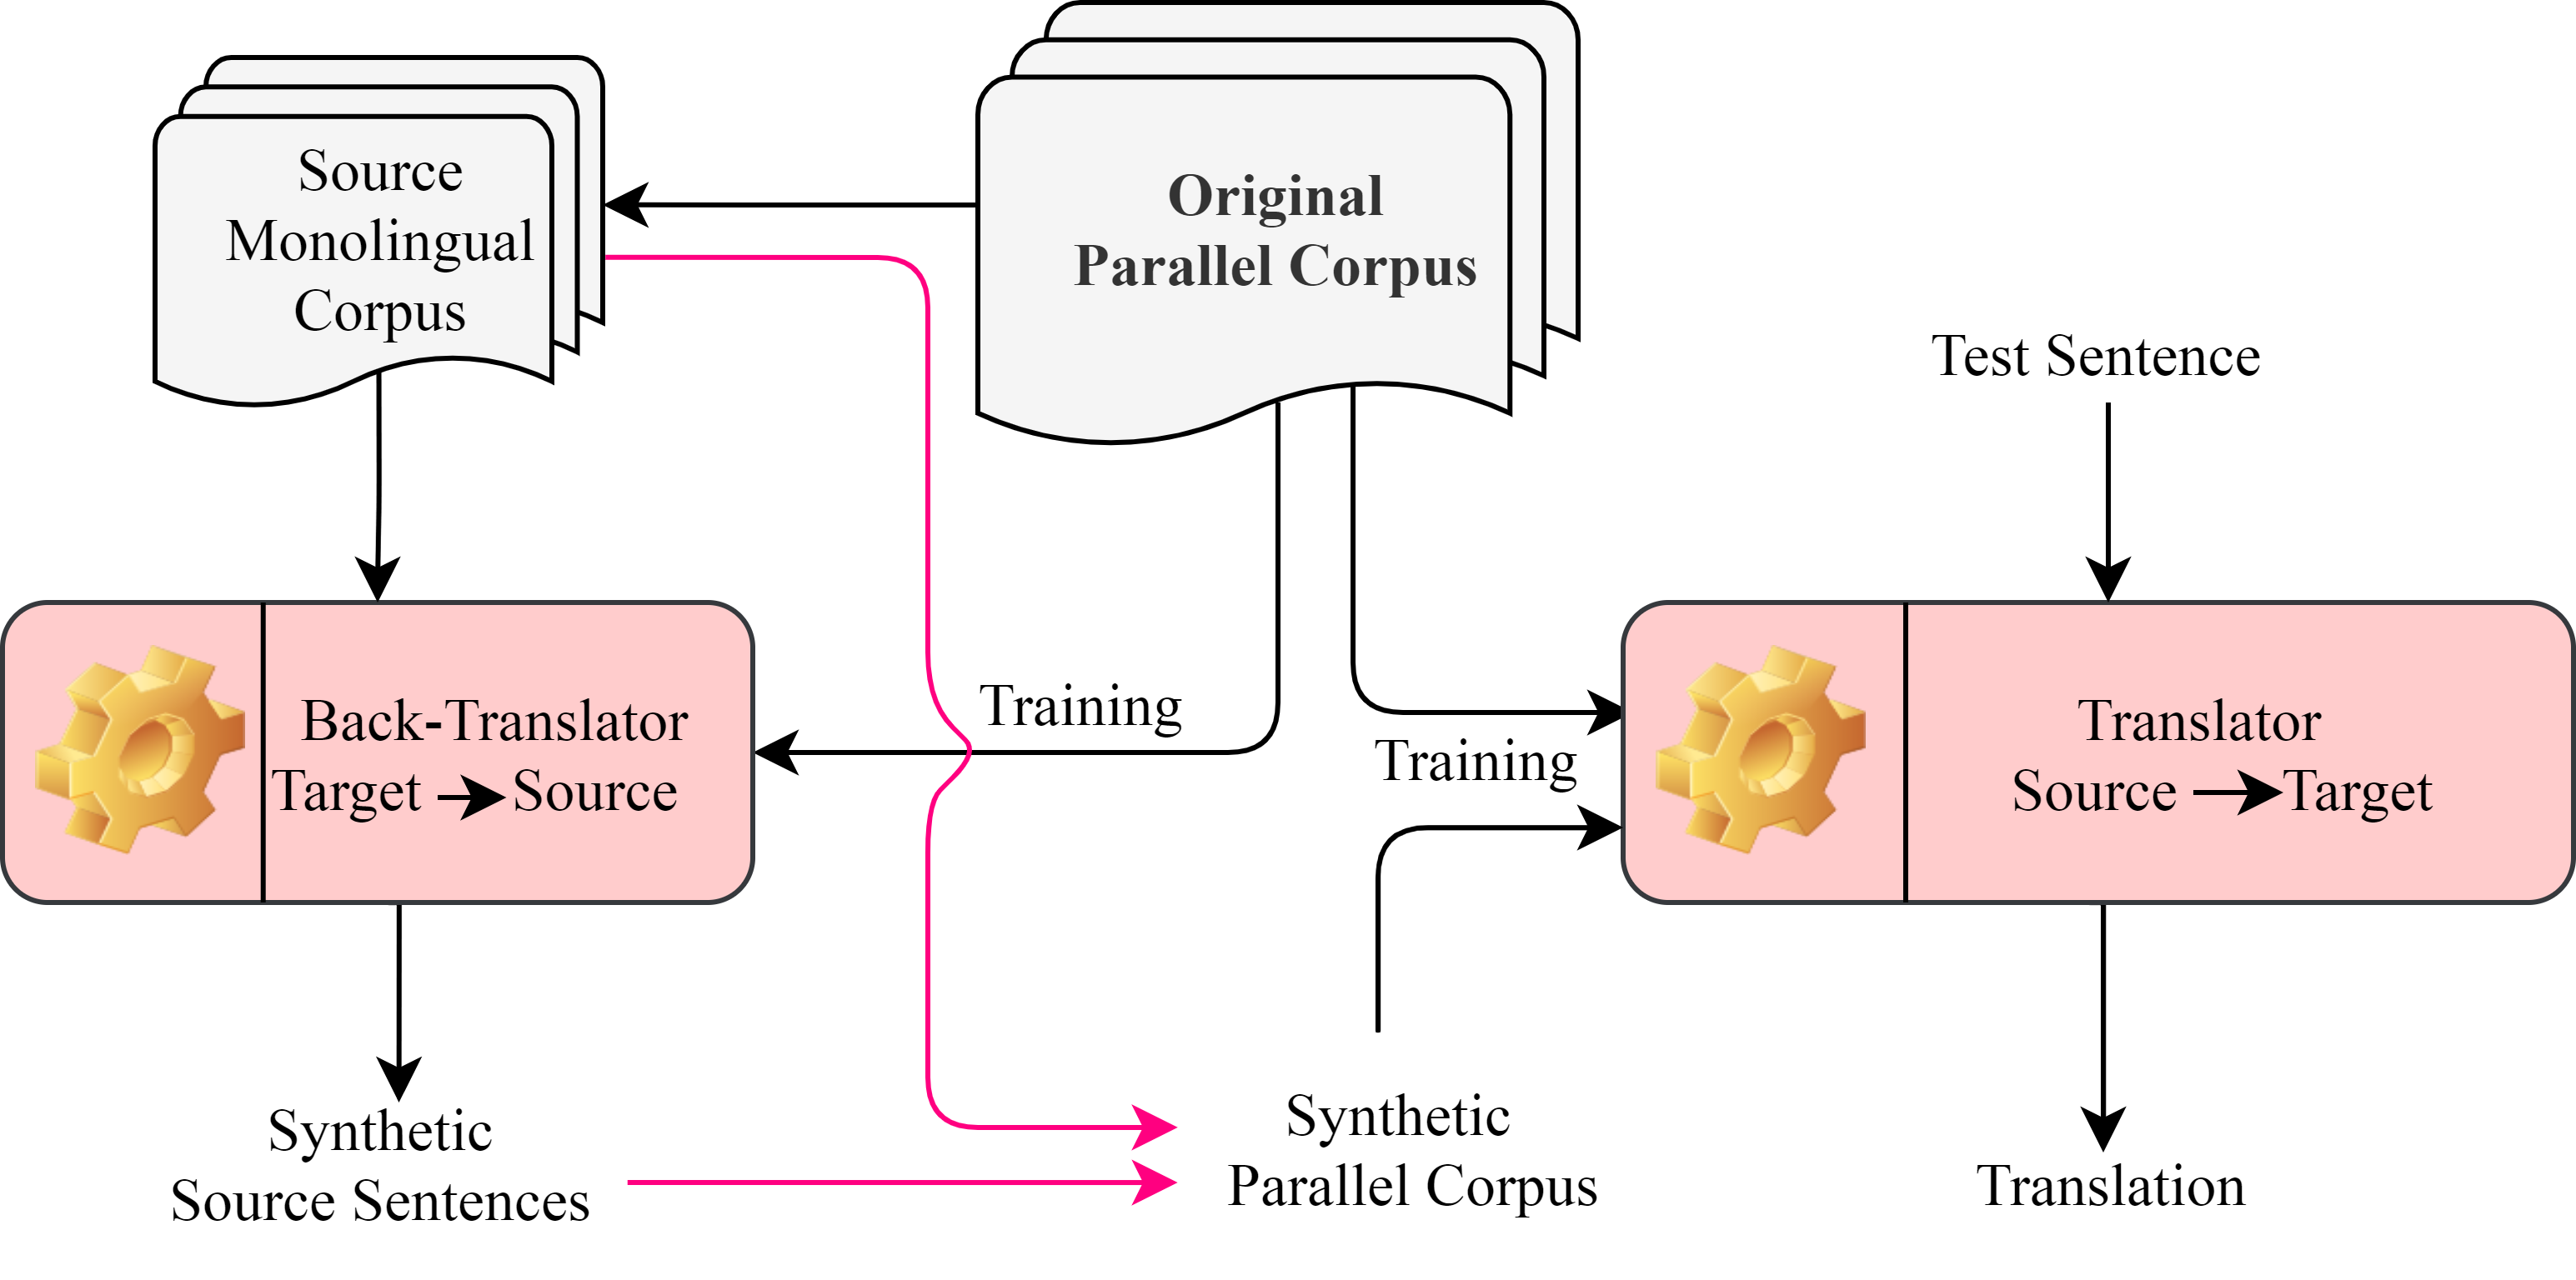
\includegraphics[width=0.9\linewidth]{selfLearning.png}
    \caption{Self training}
    \label{self-training}
\end{figure}

\subsection{Multi-task learning}
A subarea of transfer learning is multitask learning, where the target and source tasks are treated the same and learned simultaneously. In multi-task learning, the learner receives information about multiple tasks at once compared to transfer learning, where the learner initially has no idea about the target task. Multi-task learning emphasizes generating benefits for learning performance improvements in all related tasks, and information flows smoothly among all tasks developing them altogether (refer figure \ref{TLvsMTL}). Tasks like multiword expression detection and part-of-speech tagging have been found very useful for others like chunking. High resource tasks may be preferred over low-resource ones in Multi-task learning \citet{dou2019investigating}. Whereas, transfer learning focuses only on the performance of the child task (not parent task). Taking the intuition of multitask learning strategy by learning the structure of a language through syntactic parsing and part-of-speech tagging improves the performance of tasks like machine translation \citet{kiperwasser2018scheduled}. Transfer learning and multitask learning have achieved great success in many different NLP application areas, especially in machine translation over the last decades.

\begin{figure}[!h]
  \centering
  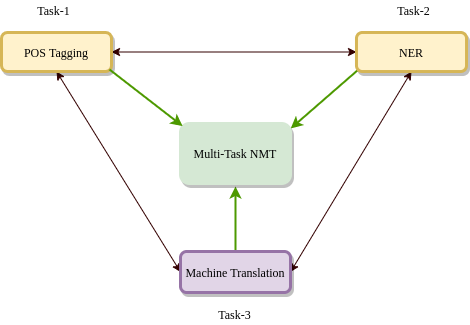
\includegraphics[width=0.5\linewidth]{nmtMultitask.png}
  \caption{Multitask Learning}
  \Description{}
  \label{TLvsMTL}
\end{figure}

\subsection{Multilingual learning}
The general framework of encoder-decoder networks decomposed into two modules makes it possible to build a system that maps a source sentence of any language to a common continuous representation and decodes its representation into any of the target languages. The mapping from multiple source languages into multiple targets in a multilingual translation model has been accepted in recent times and gained recognition due to the advantage of positive transfer between high- and low-resource language pairs. Different configurations (refer \ref{multilingual-configuration}) of multilingual models have based on the number of languages, either single or multiple source/target languages, under consideration.
\begin{figure}[!h]
  \centering
  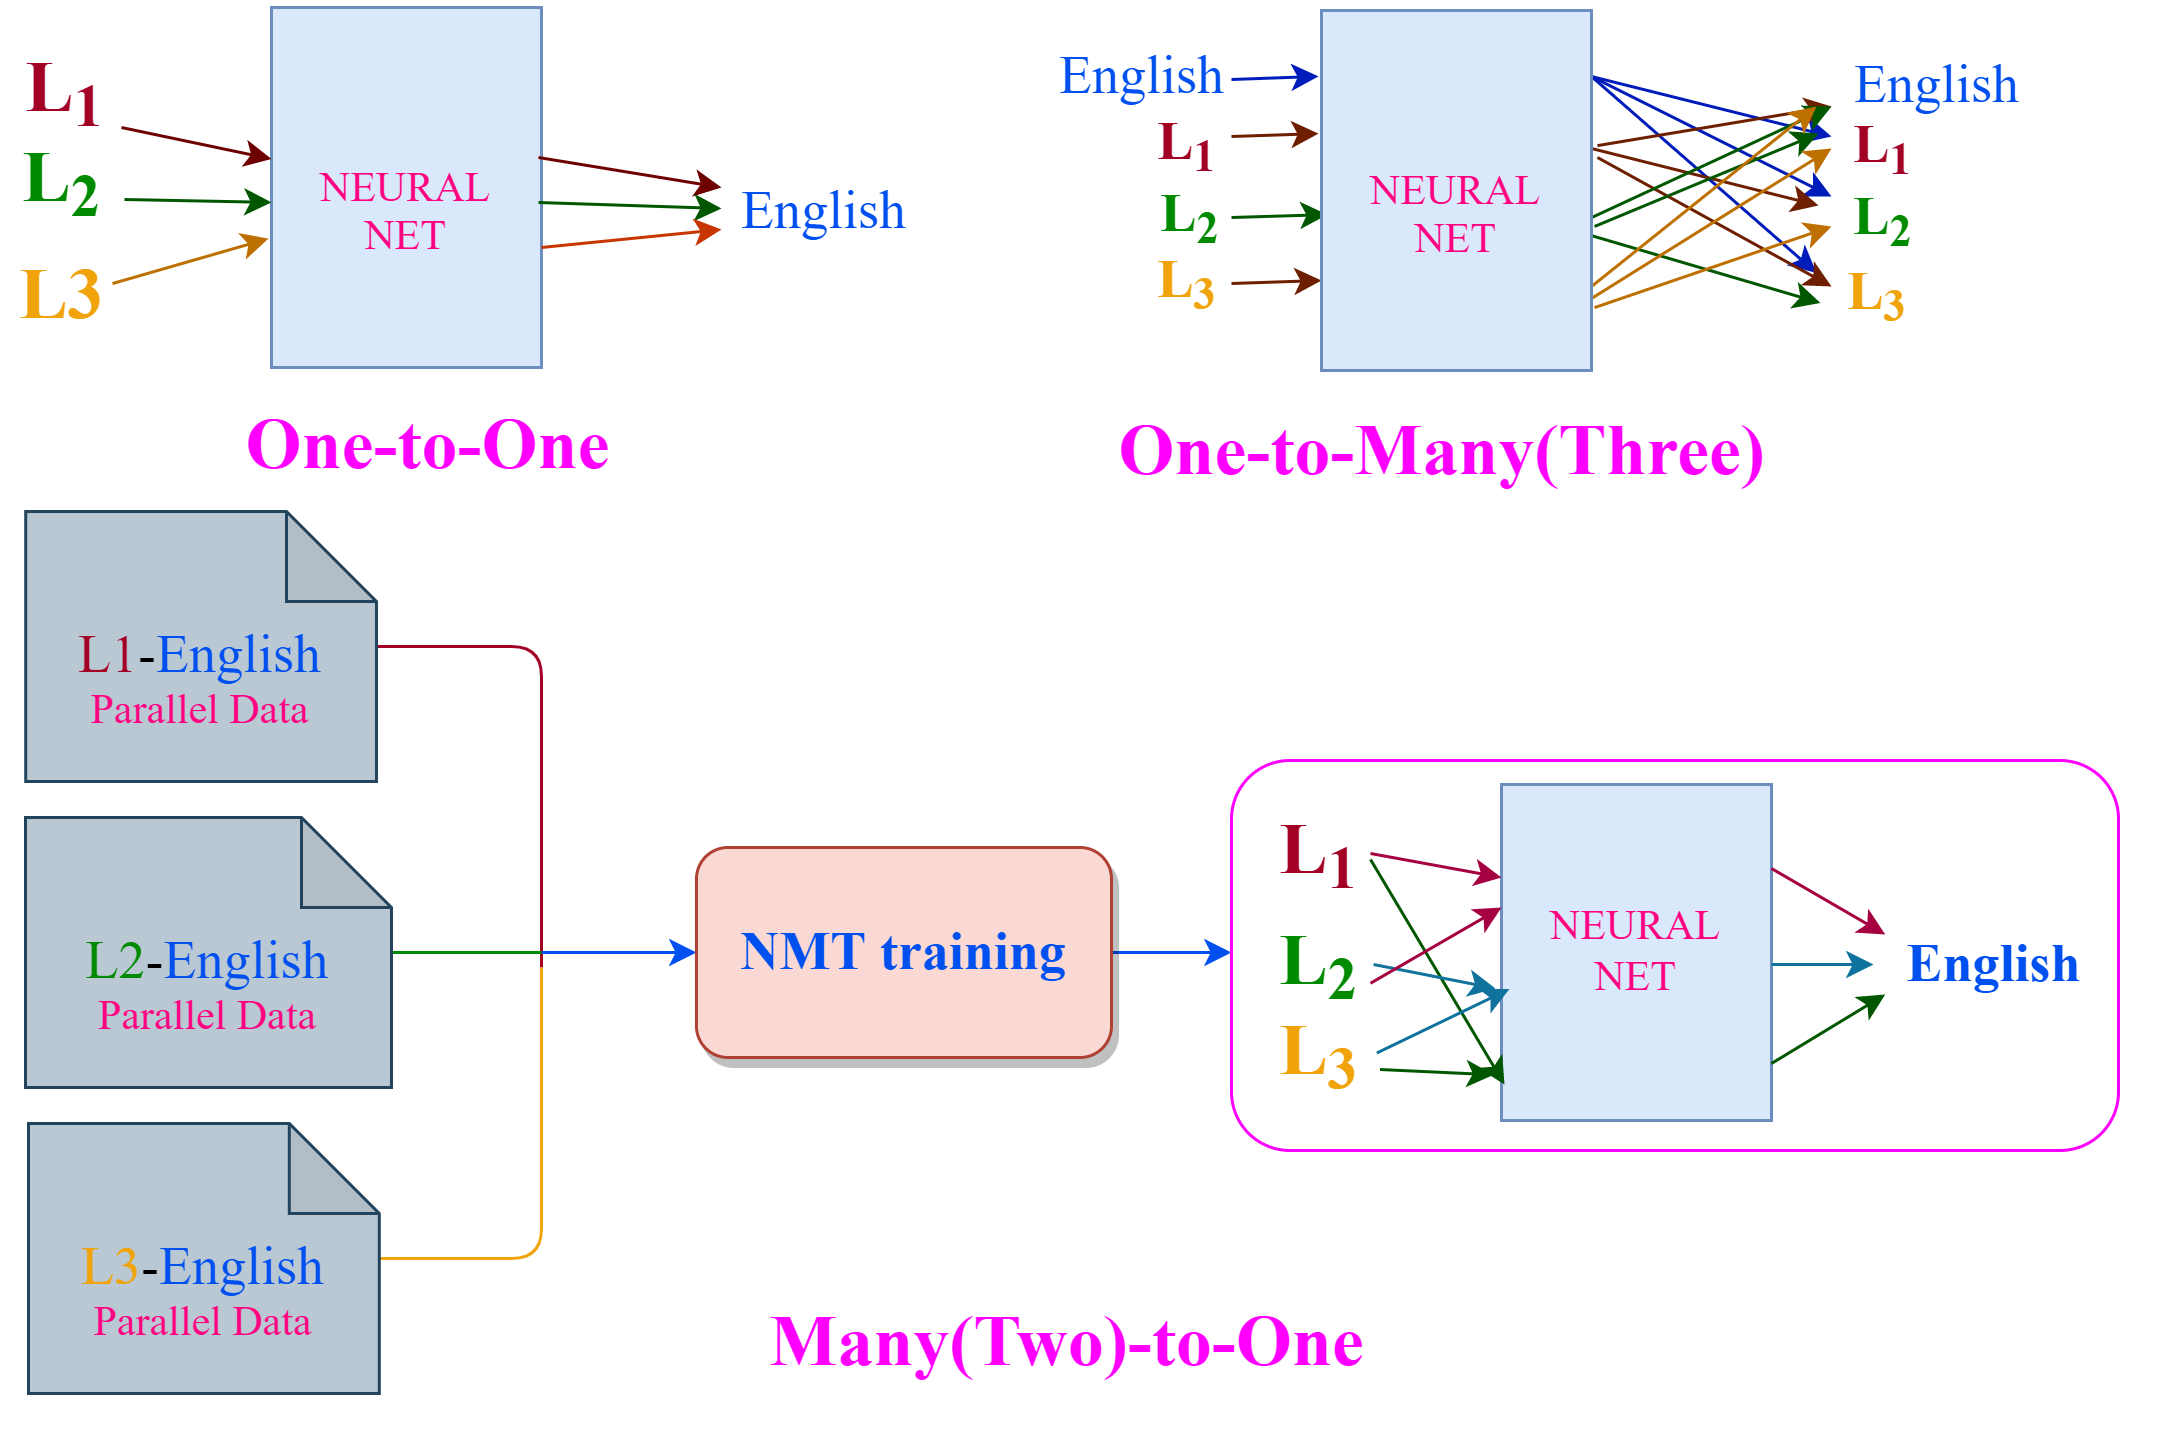
\includegraphics[width=0.9\linewidth]{MultilingualConfiguaration.png}
  \caption{Multilingual Configuration}
  \Description{Multilingual Configuration}
  \label{multilingual-configuration}
\end{figure}
NMT provides an ideal setting towards a multilingual MT as the model's parameters can be easily and efficiently shared and several similarities are detected by the model in the embedding and hidden layers.

That way, MultLin-NMT exploits improving the performance of NMT systems for low-resourced languages. To improve the translation quality of LRL, \citet{gu2018universal} proposed a model of universal encoder-decoder networks with shared embedding spaces.

\subsection{Meta learning}
Machine learning algorithms used to learn how to learn in which parameters would be the most appropriate ones for a given problem. Its goal is to learn a general model that can fast adapt to a new task given a little training sample, without requiring to be retrained from scratch. Learning-to-learn or meta-learning attempts to solve the problem of ``fast adaptation on new training data''. 
Most recent approaches to meta-learning focus on few-shot learning and broadly categorized as optimization-based methods, memory-based methods and metric-based methods. Two more categories of meta-learning are 1) learning a meta-policy for updating model parameter, and 2) learning a proper parameter initialization for fast adaptation parameters. 

In meta-learning, using auxiliary high-resource language pairs, the algorithm finds the initialization by repeatedly simulating low-resource language scenarios. \citet{dou2019investigating} investigates the model-agnostic meta-learning (MAML) algorithm and its variants for low-resource natural language understanding tasks to achieve sub-optimal performance in low-resource scenarios and validate the methods by GLUE benchmark that outperform several strong baselines. \citet{mi2019meta} proposes a generalized optimization-based approach (Meta-NLG) based on the MAML algorithm that significantly outperforms other training procedures in various low-resource configurations and demonstrates extremely fast and well to low-resource situations. A standard supervised, zero-shot as well as few-shot cross-lingual experimental setup demonstrates the consistent effectiveness of meta-learning for a total of 15 languages used in different NLU tasks \citet{nooralahzadeh2020zero}. It shows that meta-learning can effectively leverage training data from an auxiliary language for zero-shot and few-shot cross-lingual transfer. 

MAML (~\citet{finn2017model}) provides a general approach to adapting parameters across different domains. MAML solves few-shot learning problems by learning a proper parameter initialization. They have applied to low-resource machine translation by viewing language pairs as separate tasks. One of the techniques in meta-learning is model transfer. In neural network, the learning algorithm turns the training task into a training case. That is a training case that becomes a training task. \citet{gu2018meta} first explored the LR-NMT as a meta-learning by applying the first-order MAML, which learns to adapt to LRL based on multilingual HRL tasks. Researchers proposed a meta-learning algorithm for LR-NMT by learning a proper parameter initialization for fast adaptation. To sum up, MetaNMT can be the most useful settings to improve the results of machine translation for language pairs where the available parallel corpora are extremely small. Ensembling unsupervised, multilingual transfer and meta-learning can be useful for this.

\subsection{Transfer learning versus Multilingual learning versus Meta learning}
Traditional gradient-based networks require an enormous amount of data to learn, often through extensive iterative training. The goal of meta-learning algorithms is to endorse fast adaptation to new training data to improve on direct transfer learning by better fine-tuning. The notable difference between the TL, multilingual transfer, and meta-learning approaches intuitively contrasts in the diagram (refer figure \ref{TL-MultiL-MetaL}). There are three LRL-pairs fra-eng, spa-eng and por-eng and two target pairs are rum-eng and lav-eng. The green circles designated as low-resource languages.

\begin{figure}[!h]
  \centering
  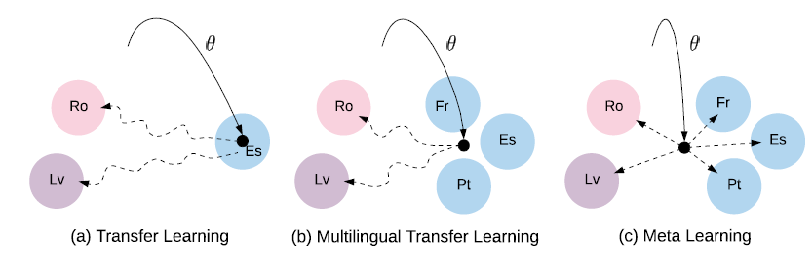
\includegraphics[width=\linewidth]{TLMuLLMeL.png}
  \caption{Transfer Learning - Multilingual Learning- Meta Learning (referred from \citet{gu2018meta})}
  \Description{learning process of Transfer Learning}
  \label{TL-MultiL-MetaL}
\end{figure}

Figure \ref{TL-MultiL-MetaL} (a) shows that TL trains an NMT system specifically by the source language pair (spa-eng) and then fine-tunes each of the target pair rum-eng and lav-eng. Transfer learning does not take into account subsequent learning.
Figure \ref{TL-MultiL-MetaL} (b) shows that multilingual often trains a single NMT system that can handle many different pairs (fra-eng, spa-eng, and por-eng), which may or may not include target pairs rum-eng and lav-eng. If the target pairs is increased, then fine-tune each of them as TL. The multilingual transfer approach does not consider how learning happens with the target. The multilingual learning does not take into account new future task. From the above analysis, we can say that both the TL and multilingual transfer learning are only interested in the source task. In meta-learning, figure \ref{TL-MultiL-MetaL} (c) shows fine-tune both the source and target task. The meta-learning aims at learning a proper initialization that can be adapted to any task with minimal training samples and explicitly incorporates the learning process within the framework. The meta-learning considers subsequent learning on a new future task.

\subsection{Zero resource translation: pivot-based and zero-shot translation}
Multilingual NMT makes a single model that understands different language pairs with the help of multilingual machine translation. Multilingual NMT permits zero resource translation (ZRT) without direct use of source-target parallel corpora into two ways: implicitly-learned bridging (zero-shot MT) and explicit bridging or interlingual translation (pivot based MT).  
The scenario where two languages have little or no parallel data between them but well connected through a third language is called pivot language. They independently transfer from one (source) to another (target) language by translating from the source language to the pivot language and then from the pivot language to the target language. The dotted lines tagged with PT from J to K and K to J via language E denotes the pivot-based translation (refer figure~\ref{TL-ZST-PT}).

\begin{figure}[!h]
    \centering
    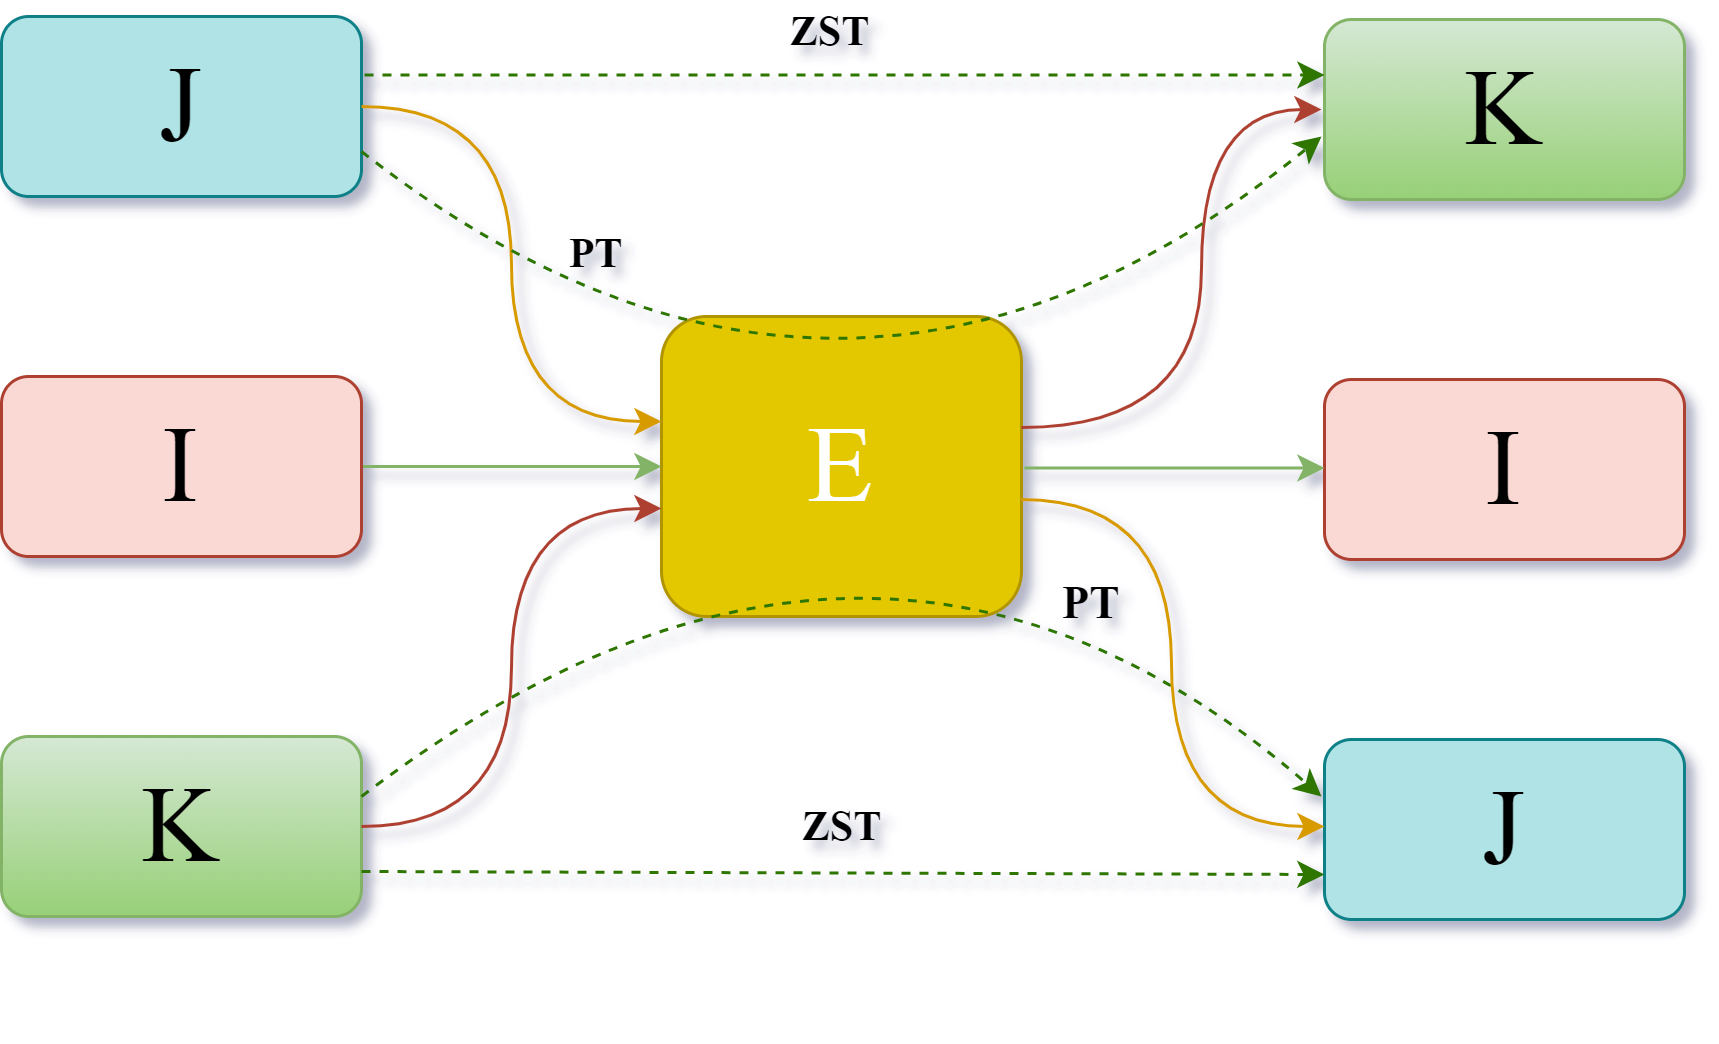
\includegraphics[width=0.6\linewidth]{ZSTPTcurved.png}
    \caption{Zero-shot and Pivot translation (here I, J, K and E 
    as placeholders to denote arbitrary languages)}
    \Description{where I, J, K and E 
    as placeholders to denote arbitrary languages}
    \label{TL-ZST-PT}
\end{figure}

In pivot-based approaches bridging source and target languages, there exist in-hand source-pivot and pivot-target parallel corpora, which used to train source-to-pivot and pivot-to-target translation models, respectively. 
Instead of solving the ZRT by a two-step process of pivoting or bridging through a common language, the idea of zero-shot translation (ZST) has a single MT engine (multilingual NMT) built by concatenating multiple parallel sentence pairs in several language directions. The engine learns to encode the inputs with several distinct languages into an underlying vector representation, and generate the output based on the encoder representation. 
The Universal language model achieves reliable results across most languages in NMT and is the state-of-the-art for Zero-Shot models. This technique is faster to train, and a single model (simplicity) can support hundreds of languages with inadequate training resources. Google's multilingual NMT system allows a single system to translate between multiple languages that enable ZST. From a trained, multilingual system referred from figure~\ref{TL-ZST-PT}, consider the translation direction as J$\leftrightarrow$E and K$\leftrightarrow$E language pairs, where J, K, E are different languages. Sharing parameters of these language pairs enables the system to transfer the translation knowledge from one language to another. The multilingual training forces system a translation between K$\leftrightarrow$J, where K$\leftrightarrow$J examples not shown during training. The dotted line tagged with ZST from J to K and K to J depicts the zero-shot translation.
Google system potentially leveraging the available parallel data from other multiple language pairs and without following the pivot scenario capable of building connections across arbitrary language pairs for which was trained before.

\subsection{Multi-modal on NMT (MMNMT)}

With the success of deep neural networks (DNN), the tasks of natural language processing (NLP), computer vision (CV) and speech processing by the use of input signal as mono-modal such as characters or words or phrases, images or videos and audio signals have improved. The researchers have designed a multi-modal system to alleviate several modalities for more extensive generalization ability. A multi-modal architecture can serve multiple input modalities. NMT is a data-driven procedure, could be challenging in this context.\\
Improving the accuracy of machine translation exploits not only the input text itself but also various background information related to the text from other modalities that could find the real sense of ambiguous words in the source sentence. A lot of work shown on NMT by different modalities that can benefit neural machine translation, such as multi-modal attention mechanism focuses on an image (\citet{caglayan2016multimodal, heo2019multimodal}), incorporate spatial visual information into the multi-modal NMT model (\citet{calixto2017doubly,huang2016attention, zhou2018visual}) and unsupervised multi-modal NMT (\citet{huang2020unsupervised}). There are several Multi-modal MT challenge at WMT, such as visual information in the multi-modal translation  (\citet{parida2019idiap}), using image information for re-ranking the translation candidates in multi-modal cross-lingual word sense disambiguation models (\citet{ lala2018sheffield}), and text supplemented by an image on multi-modal machine translation (\citet{barrault2018findings, elliott2017findings, specia2016shared}). Neural machine translation can perform satisfactory results with multi-modal, multilingual, and multidomain data.\\

\subsection{Active learning in neural machine translation}
Active learning or query learning is a subset of machine learning that extracts specific information to solve a real-time problem. It focuses on the domain of interest. The learning algorithm has the liberty to choose the data from where to learn. It is a fact that labeled data are difficult to procure, whereas unlabelled data are readily available.  From the huge unlabelled pool, the ML algorithm asked the relevant query to the Oracle (an annotator) and the extracted information is then stored into the original training set. After many iterations, leverage the existing labeled (and new) data until it becomes sufficient for processing the task. Uncertainty based sampling matrices are used to evaluate the performance of active learning. Broadly, the active learning falls into two types: stream-based selective setting assume that getting an unlabelled instance is free and pool-based active learning setting assumes that there is a large pool of unlabelled data. Based on the assumption, the former select each unlabelled instance one at a time and decide whether it wants to query the label of the instance or reject it based on its informativeness. In pool-based active learning, examples are drawn from the pool according to some informativeness measure. The active learning query method is one of the significant areas in modern-day machine learning research. One of the most popular areas in active learning is NLP that requires lots of labelled data. 
A sufficient bilingual corpus is required to train an NMT model for high-translation quality. Many low-resource language pairs are short of large scale parallel corpora, and developing such parallel corpora is rather expensive.
Active learning provides semi-supervised methods to reduce the cost of data procurement. Active learning into NMT (\citet{zhang2018active}) considers the semantic similarity according to the characteristics of NMT. The proposed active learning approaches semantic similarity and decoder probability experiments on Indonesian-English and Chinese-English presents that selection approaches are superior to random selection and other conventional selection methods.
Active learning can be used for more linguistic features to measure differences between sentences and explore to deal with low resource problems.

\section{Summary of surveyed approaches/techniques to low-resource neural machine translation}
\label{summarized}
\subsection{Traditional approaches to low-resource neural machine translation}
In this section briefly discussed a few approaches and techniques to circumvent many challenges and demonstrate the utility for low-resource neural machine translation system.
\subsubsection{\bf{Handling rare words}}
Translating with low-frequency words for low-resource and highly-inflected languages is one of the challenges in NMT \citet{koehn2017six,ngo2019overcoming}. \citet{ngo2019overcoming} explored this issue by three different strategies in NMT, first low-frequency word translation by integrating source embeddings to the attention component of NMT, second by presenting a supervised approach (separating affixes algorithm) for reducing unknown words, and third dealing with OOV (words occurring in test data but not in the training data) by leveraging the linguistic information from the wordnet. Challenging the issue of mistranslating rare words in NMT of low-resource languages (LR-NMT), \citet{ngo2019overcoming} proposed two solutions $\colon$ one for normalizing some matrices by fixing to constant value after several training epochs and another to generate a target word based on source word (s) by jointly training a simple feed-forward neural network (FFNN) with rest of the NMT model. \citet{fadaee2017data} proposed low-frequency word to replace a common word in the target text and the corresponding word changed in the source sentence to improve translation quality of rare words. Conventional NMT systems have their inability to successfully translate OOV words mainly on the low-resource of the parallel corpus. Sub-words can handle the weakness of NMT model and show potential advantages (\citet{sennrich2016neural,wu2016adapting}). A word which is not seen in the vocabulary of the input text (called unknown word) is mapped to a special token (UNK) in NMT systems (\citet{jean2015using,luong-etal-2015-addressing}). \citet{wu2016adapting} proposed a sub-words model to address the OOV problem in attention-based NMT model for LRL. \citet{sennrich2016neural} proposed to reduce unknown words using Gage’s Byte Pair Encoding (BPE) algorithm (\citet{gage1994new}).


\subsubsection{\bf{Data augmentation}}
A primary trend is expanding LRL datasets by applying augmentation methods. Data augmentation is exploiting monolingual corpora of same language or parallel data involving other language pairs.
The challenge of insufficient parallel data tackled by using a semi-supervised NMT approach which requires a few thousand parallel sentences for an extremely low-resource language to achieve a high-quality machine translation system. There have been several attempts on incorporating the monolingual corpora (on both source and target side) into NMT that improve the quality of machine translation systems. Parallel corpora are usually limited in quantity, quality, and coverage, especially for low-resource languages. It effectively becomes a semi-supervised setting \citet{cheng2016semi,wang2019semi} that takes the advantage of both labeled (insufficient parallel) and unlabeled (abandoned monolingual) data. \citet{skorokhodov2018semi} investigated ways of combining translation model with language models as semi-supervised approach. Despite being ``unlabeled'', monolingual corpora it still exhibit rich linguistic structure of a language. \citet{gulcehre2015using} investigate to leverage the available target side monolingual corpora to augment the decoder with a language model for LRL-pairs (\citet{baziotis2020language}). They showed to improve the translation model by shallow or deep fusion of separately trained language model. \citet{sennrich2016improving} proposed two strategies for low resource NMT by making use of monolingual data to fill the source side of monolingual training instances: using a ``dummy source sentences and ``synthetic source sentences'' via an effective data-augmentation scheme BT. There are promising improvements by using the target-side monolingual data. 

\subsubsection{\bf{Back-translation and Cross-lingual word embedding}} Using both source and target monolingual corpora as similar to semi-supervised method \citet{cheng2016semi} have explored to add an auxiliary autoencoder for reconstructing the monolingual corpora, which brings back the original one from the translated sentence. An effective approach is to create a synthetic parallel corpus by back-translating a monolingual corpus in the target language (\citet{sennrich2016improving}).
\citet{currey2017copied} adding target-side monolingual training data to an NMT system without changing its architecture or training algorithm. Here, augmenting the training data by coping directly from target language text improves the performance of LRL. \citet{ramachandran2017unsupervised} presented a unsupervised method by initializing the pretrained weights of two language models to the weight of encoder-decoder and then fine-tuned with labeled data.

Cross-lingual word embedding mappings have attracted a lot of attention for data augmentation in NMT (\citet{mi2020loanword}). The previous methods can be broadly classified into two categories: a) joint methods, which simultaneously learn word representations for multiple languages on parallel corpora \citet{luong2015bilingual}, and b) mapping methods, which independently train word embeddings in different languages and map them to a shared space through linear transformations (\citet{mikolov2013exploiting,artetxe2018generalizing}). Most of the recent research has focused on mapping methods because of little or no cross-lingual signal (\citet{zhang2017adversarial,conneau2017word,artetxe2018generalizing}). The need of cross-lingual embeddings is to bridge the divergence among languages. It can apply to leverage the high-resource of one language (e.g. English) in solving problems of low-resource languages (e.g. Assamese, Odiya etc.). Sharing multilingual embedding in a vector space can possess some association or correlations between them. Cross-lingual word embeddings represent words from multiple languages in a common vector space. A completely unsupervised approach proposed by (\citet{artetxe2017unsupervised}), trained the NMT system only by monolingual corpora using a combination of denoising, and backtranslation. Unsupervised cross-lingual embeddings, assuming the distribution of words in different languages is approximately the same, means one language can be mapped with other language embeddings, then languages share an isometry between words. \citet{conneau2017word} proposed complete unsupervised approach to cross-lingual mapping to word translation without parallel data. We reviewed some of the techniques of traditional approaches to LR-NMT and suggested future research directions as in Table~\ref{TradAppLRL-NMT}.

\begin{longtable}{|p{0.03\textwidth}|p{0.25\textwidth}|p{0.25\textwidth}|p{0.20\textwidth}|p{0.2\textwidth}|}
\caption{\bf{Traditional approaches to low-resource neural machine translation}}
\label{TradAppLRL-NMT}
\multicolumn{5}{c}{} \\ \hline
  \textbf{P. Id.} & \textbf{Techniques/solution features} & \textbf{Language(s)/ pair (LRL) with corpus statistics} & \centering \textbf{Contribution} & \textbf{Future research} \\
    \hline
     \newline \newline \centering \rotatebox{90} {\citet{ngo2019overcoming} }
&
    Integrating source embeddings to the attention component, using WordNet, and separating affixes algorithm.
&
    $\bullet$ Lang-pairs$\colon$ jpn-vie from TED (WIT3) with 106758 sentence pairs and eng-vie from IWSLT 2015 with 133K sentence pairs. \newline
    $\bullet$ Beat existing SOTA by +1.0 BLEU for jpn-vie NMT systems.
&
    $\bullet$ Reduce the number of unknown words for the eng$\rightarrow$via translation system using supervised algorithm. \newline 
    $\bullet$ Leveraging linguistic information from WordNet.
&
    Exploiting monolingual corpus with unsupervised methods. \newline 
    Select from n-best synonymous words for SRC sentence.\\
    \hline
     \newline \newline \centering \rotatebox{90} {\citet{nguyen2018improving}}
&
    $\bullet$ Fix the norms of context vectors and embeddings by constant. \newline 
    $\bullet$ Integration of a simple lexical module. \newline 
    $\bullet$ Applied post-processing on TGT translation's UNK through the SRC word according to highest attention score.
&
    $\bullet$ Lang-pairs: \{tam, urd, hau, hun, tur, uzb\}-eng and eng-\{jpn, vie\} \newline 
    $\bullet$ Data sizes from 100K words to 8M words. \newline
    $\bullet$ Improvements of up to +4.3 BLEU on normalization approach and lexical model.
&
    $\bullet$ Explore the mistranslated rare words in NMT. \newline 
    $\bullet$ Surpassing phrase-based translation in nearly all settings.
&
    NMT equipped with this methods is more viable choice for LR translation.\\
    \hline
    \newline \newline \centering \rotatebox{90} {\citet{fadaee2017data}}
&
    $\bullet$ TDA targets low-frequency words by generating new sentence pairs. \newline 
    $\bullet$ By leveraging language models trained on large amounts of monolingual data.
&
    $\bullet$ Lang-pairs$\colon$ eng$\leftrightarrow$ger of WMT15 training data.  \newline
    $\bullet$ Translation quality up to 2.9 BLEU points over the baseline and up to 3.2 BLEU over BT.
&
    $\bullet$ Label preservation alter both SRC and TGT sentences at the same time as long as they remain translations of each other. \newline 
    $\bullet$ Focus on augmenting instances involving low-frequency words and exacerbated in a LR setting. \newline 
&
    Apply another methods of data augmentation including targeted word selection, rare word substitution, translation selection, sampling etc.\\

    \hline
    \newline \newline \centering \rotatebox{90} {\citet{xia2019generalized}}
&
    $\bullet$ Data augmentation in LR-MT using TGT-side monolingual data, as well as pivots through a related HRL. \newline 
    $\bullet$ Unsupervised translation and bilingual dictionary induction.
&
    $\bullet$ LRL-HRL pairs$\colon$ aze-tur, bel-rus, glg-por, and slk-ces  \newline
    $\bullet$ Number of sentences in a range of 61K to 2M. \newline $\bullet$ Improve translation quality by up to 1.5 to 8 BLEU points compared to supervised BT baselines.
&
    $\bullet$ Generalized data augmentation framework for utilizing training data. \newline 
    $\bullet$ New method of pivoting through related HRLs to generate pseudo-parallel data.
&
    Explore methods for controlling the induced dictionary quality to improve word substitution. \newline 
    Jointly training pivoting system and LR translation system.\\
    \hline
    
    \newline \centering \rotatebox{90}{\citet{torregrosa2019leveraging}}
&
    $\bullet$ Leveraging RBMT knowledge for improving the performance of NMT systems in an under-resourced scenario. \newline 
    $\bullet$ Adding morphological information to the source language is as effective as using subword units.
&
    $\bullet$ Lang-pairs$\colon$ eng$\leftrightarrow$\{baq, gle\} from OPUS, OpenSubtitles 2018, Gnome and KDE4 dataset. \newline
    $\bullet$ All models are statistically and significantly better than RBMT.
    % Simplified Chinese (1M parallel entries)
&
    $\bullet$ Approach grants total control over the output of the system. \newline 
    $\bullet$ Direct usage of the lexicon entries by a) ambiguity classes and b) external information. \newline 
&
    $\bullet$ Extraction of RBMT knowledge and the inclusion of transfer rules. \newline 
    $\bullet$ Leverage information contained other RBMT systems (e.g. Apertium). \\
    \hline
    
    \newline \newline \centering \rotatebox{90} {\citet{zhou2019handling}}
&
    $\bullet$ Data augmentation via reordering according to grammatical rules, followed by word-by-word translation to create pseudo-parallel data.\newline 
    $\bullet$ First reorder monolingual TGT sentences to create SRC-ordered TGT sentences then replace the words in the reordered sentences with SRC words using a bilingual dictionary, and add them as the SRC side pseudo-parallel corpus.
&
    $\bullet$ Lang-pairs$\colon$ jap-to-eng (simulated LR, 400K parallel pairs), uig-to-eng (real LR 3088 sentences) from Bible and Wikipedia. \newline 
    $\bullet$ Significant improvements over other semi-supervised counterpart.
&
    % $\bullet$ Performance gain is not as remarkable as NMT when the amount of supervised data increases. \newline 
    $\bullet$ Word reordering-based semi-supervised models consistently outperform standard NMT models by a large margin. \newline 
    $\bullet$ Data augmentation with reordering still outperforms SMT in the case of less supervised data.
&
    Explored with different re-ordering techniques.\\
 \hline

   \newline \newline \newline \centering \rotatebox{90} {\citet{currey2017copied}}
&
    $\bullet$ Adding target-side monolingual training data to an NMT system without changing its architecture or training algorithm. \newline 
    $\bullet$ Copy the target monolingual data to the source side and use the copied data for training NMT. \newline 
    $\bullet$ Employs an autoencoder, but rather than concatenate two NMT systems flattened them into one standard NMT system. \newline
    $\bullet$ Approach is related to multitask systems with single shared encoder.
&
    $\bullet$ Lang-pairs$\colon$ eng$\leftrightarrow$tur (200K), eng$\leftrightarrow$rum (600K), eng$\leftrightarrow$ger (5M) from WMT16,17 and tur$\rightarrow$eng, rum$\rightarrow$eng translation tasks, gains of up to 1.2 BLEU over a strong baseline with BT.
&
    $\bullet$ Method proves an effective way of incorporating monolingual data into LR-NMT. \newline 
    $\bullet$ Improved accuracy by copied corpus method on named entities and other words that should remain identical between the SRC and TGT languages.
&
    $\bullet$ Explore effects of quality of monolingual data, as copied corpus technique might pose the risk of adding noise to the NMT system. \newline 
    $\bullet$ Find an effective way of adding source monolingual training data.\\
    \hline
    \newline \newline \centering \rotatebox{90}{\citet{song2020pre}}
&
    Leverage monolingual corpora of other languages to pretrain NMT models for low-resource language pairs.
&
    $\bullet$ jpn–eng (3M) translation from ASPEC and LRL settings (3K, 10K, 20K and 50K) out of 1M. \newline   $\bullet$ 0.1 to 1.5 BLEU improvements over the baseline (using unrelated assisting languages) and 2 to 2.7 BLEU improvements (using related Chinese and French)
&
    $\bullet$ Novel study for NMT pre-training by leveraging monolingual corpora of related and unrelated languages. \newline $\bullet$ Using similar assisting pairs Chinese and French and distant assisting language pairs Russian and Arabic. \newline 
&
    Increase relatedness between pre-training corpora using dictionaries and advanced unification/ mapping techniques.\\
\hline
    \newline \centering \rotatebox{90}{\citet{sennrich2016improving}}
& 
    $\bullet$ Improving neural machine translation models with monolingual data. \newline
    $\bullet$ SRC to TGT model is applied to source sentences to generate inputs via BT for training the TGT to SRC model.
&
    $\bullet$ Lang-pairs$\colon$ tur$\rightarrow$eng (320K) from IWSLT14 [+2.1 to 3.4 BLEU] and eng$\rightarrow$ger from WMT15 and IWSLT15 [+2.8–3.7 BLEU].
&
   $\bullet$ Mixing monolingual target sentences into the training set. \newline 
   $\bullet$ Source side of monolingual training instances and source sentence obtained via BT. \newline 
   $\bullet$ NMT models fine-tuning with either monolingual or parallel in-domain data.
&
    Explore how sensitive NMT training with synthetic data is to the quality of the BT.\\
  \hline
    \newline \newline \centering \rotatebox{90} {\citet{hoang2018iterative}}
&
    Iterative BT$\colon$ generating increasingly better synthetic parallel data from monolingual data.
&
   $\bullet$ The dataset obtained simulated setting eng-fre WMT (100K/1M) and realistic setting with eng-fas from LDC and TED (100K). \newline  
   $\bullet$ BLEU improvement on eng$\rightarrow$far by +0.3, far$\rightarrow$eng by +0.4, eng$\rightarrow$fre by +1.4 and fre$\rightarrow$eng by +3.1.
&
    Creating synthetic corpus by IBT improved the performance of NMT in both LR and HR scenarios.
&
    Unify various approaches BT, iterative BT, co-training, and duel learning in single framework.\\
 \hline
     \centering \newline \newline \rotatebox{90}{\scriptsize{\citet{przystupa2019neural}}}
&   
    $\bullet$ Leveraging monolingual data to improve NMT systems for similar lang-pairs using BT. \newline
    $\bullet$ Two NMT models are considered-- LSTM+Attn and transformer
&
    $\bullet$ Lang-pairs$\colon$ spa-por ($\approx$3.5M), cze–pol ($\approx$1.7M), and hin-nep ($\approx$68K sentences) from WMT19. \newline 
    $\bullet$ hin$\leftrightarrow$nep more closer BLEU than spa$\leftrightarrow$por and cze$\leftrightarrow$pol.
&
    $\bullet$ WMT19 Similar Language Translation shared task. \newline $\bullet$ Tuning the correct amount of included synthetic data is still much dependent on the size of data at hand (which can be limited).
&
    Perform BT in different contexts, with varying degrees of resource availability.\\
  \hline
    \newline \newline \centering \rotatebox{90}{\citet{ahmadnia2020impact}}
&
    $\bullet$ Cost function encodes word similarity as distances within a word embedding space. \newline $\bullet$ In a semantic space, it calculates a weighted average of distance between a reference word and all other target words. 
&
   $\bullet$ LRL pair: per-spa (1M) from OpenSubtitles 2018 \newline $\bullet$ HRL pair: Spanish-English from WMT 18 \newline $\bullet$ The word embeddings cost function resulted in higher BLEU than baseline and effective with a relatively small target vocabulary.
&
   $\bullet$ The word embedding cost function that generates similar words of per-spa aides due to relaxed constraints in the cost function. \newline $\bullet$ The approach encourages the decoder to select similar words when potential candidates OOV.
&   
    Calculation of an efficient cost function over target language words.\\
  \hline
    \newline \newline \centering \rotatebox{90}{\citet{gulcehre2017integrating}}
&
     $\bullet$ Incorporating monolingual training data (particularly on the target side) into NMT \newline
     $\bullet$ Integrate LM into NMT by shallow fusion and deep fusion. 
&
    $\bullet$ LRL-pairs$\colon$ tur$\rightarrow$eng from IWSLT’14 (361K) and chi$\rightarrow$eng from OpenMT’15 (436K). \newline 
    $\bullet$ tur$\rightarrow$eng compared to chi$\rightarrow$eng, greater performance improvement [+1:19 BLEU] under the deep fusion method.
&
    $\bullet$ A heavy dependency on the degree of similarity between the domain of monolingual corpora and the target domain of translation for performance improvement. \newline
    $\bullet$ tur$\rightarrow$eng similarity between the domains of the monolingual corpus and parallel corpora is higher than chi$\rightarrow$eng.
&
    Investigate the combination of shallow and deep fusion approaches \newline 
    Incorporate fusion techniques with TL approach.  \\
 \hline
    \newline \newline \centering \rotatebox{90}
    {\citet{pan2020exploiting}}
&   
    $\bullet$ Multi-source NMT approach for the LR-NMT to explicitly utilize the source-side linguistic knowledge. \newline 
    $\bullet$ Many-to-one setting in the multi-task learning, multiple encoders with one encoder per source language.\newline 
    $\bullet$ Employ additional knowledge-based encoder to incorporate external linguistic information into the NMT model. 
&
    $\bullet$ Lang-pairs$\colon$ tur$\rightarrow$eng and eng$\rightarrow$tur from WIT, TED talks, SETimes. \newline
    $\bullet$ The score improved in both pairs by +2.4 and +1.1, respectively.
&
    $\bullet$ Input embedding layer to accommodate for each word’s linguistic annotations at the word-level. \newline 
    $\bullet$ Benefit for improving the LR-NMT performance. \newline 
    $\bullet$ All the linguistic features are shared in the knowledge based encoder to make better generalization.
&
    Perform machine translation on high-resource and morphological-rich lang-pairs.\\
  \hline
  \newline \newline \centering \rotatebox{90}{\citet{nguyen2019transformers}}
&
   $\bullet$ Normalization-centric changes to enhance the training in Transformer. \newline $\bullet$ PRENORM: a pre-norm residual connections, SCALENORM: $l_2$ normalization with a single scale parameter for faster training and better performance and FIXNORM: effectiveness of normalizing word embeddings to a fixed length.
&
    $\bullet$ Five LRL pair:  glg$\rightarrow$eng (10K), slo$\rightarrow$eng (61K),  eng$\rightarrow$vie (133K), eng$\rightarrow$heb (212K), ara$\rightarrow$eng (214K) from TED Talks \newline $\bullet$ PRENORM + FIXNORM + SCALENORM significantly improves on average total +1.1 BLEU.
&
    PRENORM enables warmup-free, validation-based training with large learning rates with small batches and it is more stable and competent with low-resource settings.
&
    Investigate the relationship between POSTNORM and PRENORM using other optimizer like RADAM.\\
  \hline
   \multicolumn{5}{|c|}{ \bf{Semi-supervised approach}} \\
 \hline
   \newline \newline \centering \rotatebox{90}
    {\citet{cheng2016semi}}
&
   $\bullet$ Both SRC and TGT monolingual data for NMT through reconstructing the monolingual corpora using an autoencoder. \newline
   $\bullet$ Jointly trains SRC$\leftrightarrow$TGT translation models. \newline 
   $\bullet$ Semi-supervised learning model$\colon$ concatenation of labeled and unlabeled data.  
&
   $\bullet$ Lang-pairs$\colon$ chi-eng from NIST datasets (2.56M), Monolingual$\colon$ chi (18.75M) and eng (22.32M). \newline 
   $\bullet$ Monolingual corpora improve eng-to-chi translation [up to +3.2 BLEU points].
&
    $\bullet$ Adding target monolingual corpus improves over using only parallel corpus for SRC to TGT translation. \newline 
    $\bullet$ Adding target monolingual corpus improves over using only parallel corpus for SRC to TGT translation.
&
    Explore the usage of both SRC and TGT monolingual data using semi-supervised reconstruction method, with  two NMTs models. \\
 \hline
    \newline \centering \rotatebox{90}{\citet{skorokhodov2018semi}}
&
    $\bullet$ Shallow fusion between translation system and language model. \newline $\bullet$ Initialization of translation system with weights from pretrained language model.
&
    $\bullet$ eng$\rightarrow$fra and eng$\rightarrow$rus (20K and 10K) from WMT europarl-v7 \newline $\bullet$ +2.2 BLEU score on eng-fra pair.
&
    Transformer with LM initialization and fusion for both the settings 20K and 10K, the eng$\rightarrow$fra and eng$\rightarrow$rus outperform the transformer result.
&
    Explore translation with longer sentences (more than 15 words).\\
    \hline
   \multicolumn{5}{|c|}{ \bf{Unsupervised approach}} \\
    \hline
    \newline \newline \centering \rotatebox{90}{\citet{lample2018phrase}}
&
    $\bullet$ Propose two model variants, a neural and a phrase-based model. \newline 
    $\bullet$ Unsupervised MT can be accomplished by leveraging (i) initialization of TM, (ii) training LM in both SRC and TGT languages (iii) iterative BT. \newline 
    $\bullet$ Goal is to train MT system without parallel sentences (monolingual corpora only). 
&
    $\bullet$ Lang-pairs$\colon$ eng-urd, eng-rum and monolingual corpus of urd (5.5M), rum (2.9M) from WMT News Crawl. \newline $\bullet$ LRLs like eng-urd and eng-rum, unsupervised methods achieve even better results than semi-supervised and supervised approaches.
&
    $\bullet$ Fully unsupervised MT, proposed a much simpler and more effective initialization method for related languages. \newline $\bullet$ Better results than semi-supervised and supervised. \newline 
    $\bullet$ Better way to leverage monolingual data for MT.
&
    Powerful language models and better initialization methods leads better model.\\
 \hline
    \newline \centering \rotatebox{90}{\citet{artetxe2018unsupervised}}
&
    $\bullet$ Unsupervised MT with monolingual corpora only for both sides. Goal is to rain MT system without parallel sentences (completely remove the need of parallel data). 
&
    $\bullet$ Lang-pairs$\colon$ fre$\rightarrow$eng [15.56 BLEU] ger$\rightarrow$eng [10.21 BLEU] from News Crawl corpus with articles of 2007 to 2013.
&
   $\bullet$ Incorporate a modified attention encoder-decoder model on unsupervised cross-lingual embeddings. \newline 
   $\bullet$ Two strategies of  unsupervised is denoising and backtranslation (on-the-fly).
&
    Explore progressively relaxing constraints during training. \newline 
    Explore and analyze other neighborhood functions for denoising.\\
 \hline
    \newline \newline \centering \rotatebox{90}{\citet{guzman2019flores}}
&
    $\bullet$ Fully supervised, weakly supervised, semi-supervised and fully unsupervised. \newline 
    $\bullet$ MT systems use any source of data namely parallel, noisy comparable, as well monolingual data in related languages.
&
    $\bullet$ Lang-pairs$\colon$ nep-eng (564K, 2.29M, 71.5M), sin-eng (647K, 3.5M, 73.16M) parallel, Comparable and monolingual corpora. \newline  
    $\bullet$ Introduce new evaluation benchmarks of very LRL-pairs. \newline
    $\bullet$ Super-NMT baselines achieve BLEU scores less than 8.
&
     $\bullet$ BLEU score is particularly low when translating into the more morphologically rich Nepali and Sinhala languages. \newline 
     $\bullet$ UNMT seems ineffective on these distant lang pairs, achieving BLEU scores close to 0.
&
    Explore initialization of the word embeddings using UNMT. \newline 
    % $\bullet$ Code available\\
  \hline
 \multicolumn{5}{|c|}{ \bf{Filtering Synthetic data}} \\
 \hline
    \newline \newline \centering \rotatebox{90}{\citet{imankulova2019filtered}}
&
    $\bullet$ Filtering the pseudo-parallel corpus using quality estimation based on sentence-level round-trip translation. \newline 
    $\bullet$ If the target sentence and its BT are similar, we assume that the synthetic source sentence is appropriate regarding its monolingual target sentence and can be included into the filtered pseudo-parallel corpus.
&
    $\bullet$ LRL-pairs$\colon$ jpn$\leftrightarrow$rus (10231) and fre$\rightarrow$mlg (106406) as MRL from OPUS. \newline
    $\bullet$ Filtered models outperform the baselines with larger margin for low-resource language pairs than high-resource language pair.
&
    $\bullet$ Filter a pseudo-parallel corpus using sentence-level BLEU and obtain a trainable high-quality pseudo-parallel corpus. \newline$ 
    \bullet$ pseudo-parallel corpus using BT outperform the bootstrapping method. \newline 
    $\bullet$ Filtering method as additional training data is useful for low-resource lang-pairs.
&
    $\bullet$ Can improve translation performance by bootstrapping. \newline $\bullet$ Improve the filtering method detect after the quality of translation by reinforcement learning.\\
 \hline
    \newline \centering \rotatebox{90}{\citet{xu2019improving}}
&
    $\bullet$ Proposed a ``Sent-BiEMB'' filtering method Noise-- weakly paired sentences from a synthetic parallel corpus generated with BT.
&
    $\bullet$ Lang-pairs: kor$\rightarrow$eng (207K) from IWSLT 2017. \newline 
    $\bullet$ ``Sent-BiEMB'' is more effective than ``Sent-BLEU'' for filtering noise in synthetic data.
&
    $\bullet$ Measured the sentence-level similarities between
    the synthetic source and the monolingual target sentence by using bilingual word embeddings. \newline 
    $\bullet$ Experiment excludes the real parallel data.
&
    Investigate and analyze the different types of noise generated by BT.\\
  \hline
    \newline \newline \centering \rotatebox{90}{\citet{adams2017cross}}
&
   $\bullet$ Using bilingual lexicon to improve language models when textual training data is limited. \newline $\bullet$ Learning cross-lingual word embeddings (CLWE) used in training monolingual language model. \newline $\bullet$ LR language modeling and language model adaptation.
&
    $\bullet$ SRC languages: jpn, ger, rus, fin and spa and under-resource: nau (2K)\newline $\bullet$ English Wikipedia (1K to 128K) and CBOW Google News Corpus (GNC) \newline $\bullet$ CLWE methods all outperform GNC \newline $\bullet$ Pre-trained CLWEs do not significantly outperform over non-pre-trained for nau language.
&
    $\bullet$ CLWEs resilient when training data of target language is drastically reduced in a simulated low-resource environment. \newline $\bullet$ language models are improved by this pre-training.
&
    Hybrid count-based promise for language modeling for low-resource languages.\\
 \hline
    \newline \newline \centering \rotatebox{90}{\citet{yu2020efficient}}
&
    $\bullet$ Reread-feedback NMT architecture (RFNMT) for using global information. \newline $\bullet$ Reread mechanism initialize the second encoder’s input by transferring the firstpass encoder’s outputs. \newline $\bullet$ Feedback mechanism process the first-pass decoder’s outputs are leveraged by a weight model and an improved gated recurrent unit (GRU).
&
   $\bullet$ LRL pair: eng$\leftrightarrow$vie (133K) from IWSLT15, eng$\leftrightarrow$ara (231K) from IWSLT17 \newline $\bullet$ HRL pair: eng$\leftrightarrow$ger (4.5M), eng$\leftrightarrow$fra (36M) from WMT14 \newline $\bullet$ LR pairs boosted BLEU with an average 1.57 over baseline.
&
    RFNMT architecture significantly outperform the baseline and state-of-the-art methods in terms of translation quality and integrity.
&
    Apply the RFNMT framework to other cross-lingual NLP tasks such as dialog generation and summarization generation.\\
  \hline
   \multicolumn{5}{|c|}{\bf{Self Training}} \\
    \hline
    \newline \newline \centering \rotatebox{90}{\citet{he2019revisiting}}
&
   $\bullet$ ST, a ``pseudo-label'' semi-supervised learning approaches. \newline
   $\bullet$ Augment the original labeled dataset with unlabeled data paired with the model's prediction.
&
    $\bullet$ WMT eng-ger dataset, 
    FloRes eng-nep (560K), Nepali mono (3.6M), and English Wiki(68M). \newline 
    $\bullet$ Noisy ST outperforms the baseline (1 $\sim{5}$ BLEU).
&
    $\bullet$ Effective method to improve generalization, particularly when labeled data is scarce. \newline 
    $\bullet$ An effective approach in low-resource setting of machine translation.
& 
   Explore self-training when the target output is natural language. \\ 
%   $\bullet$ Code \footnote{https://github.com/jxhe/self-training-text-generation} 
  \hline
    \newline \newline \centering \rotatebox{90}{\citet{shen2019source}}
&
    $\bullet$ Train models with two complimentary approach BT and self-training. \newline 
    $\bullet$ A controlled setting analyze source-target domain mismatch (STDM), and amount of dependence between parallel and monolingual data. 
&
    $\bullet$ Low-resource nep-eng dataset has used. \newline 
    $\bullet$ BT+ST (by parallel data) +2.5 BLEU than baseline and (BT+ST) +0.6 BLEU than BT.
 &
    $\bullet$ STDM (effect of local context) in MT is de facto the best known approach to leverage monolingual data in low resource settings. \newline 
    $\bullet$  ST approach better leverages in-domain monolingual data on the source side.
 &
    $\bullet$ Need better characterization of STDM. \newline 
    $\bullet$ Better algorithms leveraging to source monolingual data. \newline 
    $\bullet$ Measure semantic content of language by random partitioning constant.\\
 \hline
    \newline \centering \rotatebox{90}{\citet{imamura2018nict}} 
&
    $\bullet$ Self-training the source-side of training data to increase variety. \newline $\bullet$ Improves the accuracy without changing the model structure.
&
    $\bullet$ WMT-2014 eng-ger translation. \newline $\bullet$ Marian framework for NMT were better than those of OpenNMT.
&
    $\bullet$ The self-training approach does not effect the translation efficiency. \newline $\bullet$ This method is effective for both the transformer and seq-to-seq models.
&
   Experiment with another BT methodology.\\
  \hline
    \newline \newline \centering \rotatebox{90}{\citet{sun2020self}}
&
   $\bullet$ Self-training mechanism to generate synthetic training data for UNMT in two steps: self training with pseudo-supervised training (ST-PT) and unsupervised training (ST-UT).
&
    $\bullet$ Lang-pairs$\colon$ rum-eng and est-eng. \newline
    $\bullet$ Monolingual corpus from WMT news crawl has used for rum (8.92M) and est (3.00M). \newline 
    $\bullet$ For eng-rum (0.7-9.91), ST-PT improve over baseline, ST-UT and UNMT. \newline
    $\bullet$ For eng-est, ST-PT outperforms than ST-UT and UNMT.
 &
    $\bullet$ Explore the unbalanced training data scenario problem in UNMT.
 &
    Explore the combine effect of ST with BT for UNMT\\
 \hline
    \newline \centering \rotatebox{90}{\citet{abdulmumin2020using}}
&
    Using self-learning to improve the performance of the backward model in back-translation.
&
     English-Vietnamese (133317) from IWSLT15 [1.5 BLEU] English-German (153348) from IWSLT14 [11.06 BLEU].
&
    $\bullet$ Improve the backward and forward models instead of requiring the source and target data. \newline $\bullet$ Without data cleaning and/or freezing learned parameters, self-training improves the backward model.
&
    Explore by repeated retraining of the backward model that is iterative self training.\\
    \hline
  \bottomrule
\end{longtable}

\subsection{Knowledge transfer approaches to low-resource neural machine translation}
\subsubsection{\bf{Transfer learning}}
In transfer learning (TL), it trains a high-resource language pair as a parent model. The weights obtained from the trained model are used as the initialization for a low-resource child model and then finally trained on the small parallel corpus of the child model. The TL approach is applied in different low-resource NLP tasks in both semi-supervised and unsupervised settings. TL widely used in LR machine translation because it is one of the vital directions for approaching the data sparsity problem in LR-NMT.
\citet{zoph2016transfer} demonstrated a transfer learning approach to low-resource translation, which is a pioneer to apply on NMT. They observe significant improvements with a variety of languages, including Hansa, Turkish, Uzbek and Urdu, when the model pre-trained with French-English used as an initial point.
The parent model transfers some other vital components of neural networks such as the encoder, decoder and attention parameters to the child language, which is relatively inflective, exceptionally agglutinative in LRL-pairs in the works (\citet{zoph2016transfer,  passban2017translating, nguyen2017transfer, dabre2017empirical, maimaiti2018discussion, maimaiti2019multi, luo2019hierarchical, luo2020joint}).

\citet{nguyen2017transfer} explored by using BPE to increase vocabulary overlap to optimize the word embedding of low-resource parent language pair, but it is related to the child language pair. Experimental results showed that similar languages are suitable for improving the performance of low-resource languages.
\citet{dabre2017empirical} presented an empirical study of language relatedness through transfer learning that gave maximum impact from parent to child pairs. The crucial point is that the source language of both the parent-child model falls in the same or linguistically similar language family, a common target language with child pair is resource-poor. 
\citet{kocmi2018trivial} compared the effect of data volume and language similarity on the transfer learning method. They concluded that the data volume of high resource language is more prominent than the relatedness of language. It is observed that an attribute gained from totally unrelated language pairs, may not be significant always. In transfer learning, the size of the parallel corpus plays a prominent role than the similarity of language pairs. The choice of transfer language for machine translation depends more on the dataset size of the corpus (\citet{lin2019choosing}).
\citet{luo2019hierarchical} used a hierarchical transfer learning architecture for low-resource languages, add the intermediate layer to make full use of similar languages, which inspired by human transitive inference and learning ability.

Most recently, \citet{luo2020joint} proposed a joint BT and transfer learning method for low-resource languages. They, effectively combine the data volume advantage of high-resource languages (\citet{kocmi2018trivial}) with the language similarity advantage of intermediate languages (\citet{luo2019hierarchical}) that significantly improves the performance for low-resource languages compared to using only one of the methods.
We reviewed some of the techniques of transfer learning approaches to LR-NMT and suggested future research directions as in Table~\ref{TLAppLRL-NMT}.

\begin{longtable}{|p{0.03\textwidth}|p{0.25\textwidth}|p{0.25\textwidth}|p{0.20\textwidth}|p{0.2\textwidth}|}
\caption{\bf {Transfer learning approaches to low-resource neural machine translation}}
\label{TLAppLRL-NMT}
%  \multicolumn{5}{c}{} \\
 \hline
 \bf{P. Id.} & \bf{Techniques/solution features} & \bf{Language(s)/ pair (LRL) with corpus statistics} & \centering \bf{Contribution} & \bf{Future research} \\
 \hline
 
    \newline \newline \centering \rotatebox{90}{ \citet{dabre2017empirical}}
&
    $\bullet$ Explores different choices of parent models affect the performance of child models. \newline $\bullet$ A parent language from the same (or linguistically similar) language family as the child language will have a larger impact on transfer learning.
&
    $\bullet$ Parent-languages: \{hin, ind, tur, rus, ger, fre\} Child-languages: \{hau, uzb, mar, pun, mal, kaz, ltz, jav, sun\} and Target language English from WMT14.
&
    Resource rich language pair in which the SRC language is linguistically closer to the SRC language of the resource poor pair much better than other choices of language pairs.
&
    Apply segment attention mechanism (like BPE or WPM) by exploiting cognates in closely related languages.\\
  \hline
     \newline \newline \centering \rotatebox{90}{{\citet{passban2017translating}}}
&
    $\bullet$ Apply transfer learning (inter-language) and vocabulary adaptation.\newline 
    $\bullet$ Feed a child model with high-level translation knowledge, which comes from a parent model.\newline 
    $\bullet$ Word stem substitution and double-transfer.
&   
    $\bullet$ Parent pairs$\colon$
    tur–eng (4.50M),
    tur–eng (5.67M) and
    Child pairs$\colon$
    aze–eng (268K),             
    aze–tur (186K),       
    tur–eng (1.17M) from OpenSubtitle2016 and Tanzil.
    \newline $\bullet$ aze$\rightarrow$eng (evaluated first time for Azeri) outperform all other existing models.
& 
    $\bullet$ Model can be used any other closely related pairs. \newline $\bullet$ Two identical teachers and fine-tuning two times (double initialized NMT).
&
    Models that are trained on a pair of languages but applied to other languages\\
 \hline    
    \centering \newline \newline \rotatebox{90}
    {\citet{kocmi2018trivial}} 
&  
    $\bullet$ Simple transfer learning method with shared  vocabulary of subword units across both the parent and child. \newline
    $\bullet$ Compare low-resource and high-resource language pairs spanning two orders of magnitude of training data size.\newline 
    $\bullet$ Shows for targeting different languages and effective for fully unrelated lang-pairs.
& 
    $\bullet$ HRL pairs$\colon$ fin-eng (2.8M) and cze-eng (40.1M) and LRL-pairs$\colon$ (closely related) est-eng (0.8M) and slo-eng (4.3M) from WMT 2018.
    
            \begin{center}
        \begin{tabular}{ |c|c| } 
         \hline
         \bf{Parent} & \bf{Child} \\ 
         \hline
         eng-fin&eng-est \\ 
         \hline
         fin-eng&est-eng \\ 
         \hline
         eng-cze&eng-slo\\
          \hline
         cze-eng&slo-eng\\
          \hline
        \end{tabular}
        \end{center}
&
    $\bullet$ Removing the restriction on relatedness of the language pairs. \newline 
    $\bullet$ Method is effective also for fully unrelated language-pairs. \newline 
&
    To investigate the impact of using only the child corpus for vocabulary generation or various amounts of used sentences\\
  \hline
    \newline \newline \centering \rotatebox{90}{\citet{maimaiti2018discussion}}
&  
    $\bullet$ Mixed Transfer learning (MTL): MTL method to share vocabulary to train the NMT model. \newline 
    $\bullet$ Focuses on the investigation of International Exchange Activities (IEA) by using artificial intelligent mechanisms. \newline 
    $\bullet$ Exploit the MT and translation memory tools.
& 
    $\bullet$ Parent pairs$\colon$ ara$\rightarrow$per (5.1M), per$\rightarrow$cha (1.4M) from Subtitle2016 and Child pair$\colon$ urd$\rightarrow$cha (78.0K) from Tanzil corpora. \newline 
    $\bullet$ Low-resource data set improvements of up to 4.13 BLEU points.
&  
    $\bullet$ Full use of bilingual cognition and combine them to better develop the Human Computer Interaction (HCI).\newline 
    $\bullet$ Mitigate computation space and reduce memory consumption and time.
&
    Try to leverage on morphological poor languages.\\
  \hline
    \newline \newline \centering \rotatebox{90}{\citet{maimaiti2019multi}}
& 
    $\bullet$ Present a language-independent and straight forward multi-round transfer learning (MRTL) to exploit multiple HRLs effectively. \newline 
    $\bullet$ Reduce the difference between HR and LR, introduce a unified transliteration method for various language families.
&  
    $\bullet$ Parent pairs$\colon$ ara$\rightarrow$cha, per$\rightarrow$cha, fin$\rightarrow$cha, hun$\rightarrow$cha, and tur$\rightarrow$cha from Subtitle2016 and Child pair$\colon$ uig$\rightarrow$cha from CLDC corpora.\newline 
    $\bullet$ Improvements on the low-resource dataset of up to 5.63 BLEU points.
&   
    $\bullet$ Different parent models from various language families, groups and branches. \newline 
    $\bullet$ Investigated orthographies of parent and child lang-pairs. \newline
    $\bullet$ Select parent model according to syntactic, semantic relatedness, language structures and linguistic features.
&
    $\bullet$ Validate the effectiveness of the model to other NLP tasks. \newline 
    $\bullet$ Try to exploit other languages such as Greek, English, Russian, French, German, Italian, and Spanish. \\
 \hline
    \newline \newline \centering \rotatebox{90}{\citet{kim2019pivot}}
&
    $\bullet$ A pre-training strategies for NMT using source-pivot and pivot-target, for improvement in source$\rightarrow$target translation. \newline
    $\bullet$ Cross-lingual encoder pre-training with auto-encoding of the pivot language.
&
    $\bullet$ fre$\leftrightarrow$ger, ger$\leftrightarrow$cze as HRL, LRL, respectively and English as PVT language from WMT 2019 news translation. \newline 
    $\bullet$ +2.6\% BLEU than WMT 2019 result.
&
    $\bullet$ The improvements are valid also in zero-shot/zero-resource. \newline 
    $\bullet$ For non-English lang-pairs: lots of source-pivot and pivot-target parallel data, little (LR) or no (zero-resource) source-target parallel data.
&
    ZST combines independently existing pre-trained encoders and decoders for non-English pairs.\\
  \hline
    \newline \newline \centering \rotatebox{90}{ \citet{luo2019hierarchical}}
&
    $\bullet$ NMT model trained in the unrelated HRL pair, the similar intermediate language pair and the LRL pair. \newline
    $\bullet$ Parameters are transferred and fine-tuned layer by layer for initialization.
&
    $\bullet$ LRL: uig-chi (0.35M) and tur-eng (0.2M) 
    HRL: eng-chi (15M) \newline
    $\bullet$ Hierarchical TL improves 1.15 BLEU over transformer-big model.
&
    $\bullet$ Make full use of helpful language resources for LRL and flexible in language choice. \newline 
    $\bullet$ Significantly improves the translation performance compared with the parent-child architecture.
&
    Explore the effect of the difference and the size of the intermediate language. \\
  \hline
    \newline \centering \rotatebox{90} {\citet{luo2020joint}}
&
    $\bullet$ Joint back translation and transfer learning method for LRL. \newline 
    $\bullet$ Incorporating data augmentation methods into transfer learning architectures.
&
    $\bullet$ Lang pairs: eng-chi (15M) from UPD, tur-eng (0.2M) from WMT16 and uig-chi (0.35M) from CWMT2017. \newline 
    $\bullet$ BLEU score uig-chi [37.41], tur-eng [19.91] on hierarchical TL + BT architecture.
&
    $\bullet$ Empirical experiment achieve significant results in uig-chi and tur-eng translation in both LRL settings.
&
    Incorporate efficient data augmentation method. \\

 \bottomrule
\end{longtable}
 
\subsubsection{\textbf{Multitasking approaches to low-resource neural machine translation}}
Multitask learning is an elegant approach to inject linguistic-related inductive biases into NMT, using different auxiliary tasks such as syntactic and semantic tasks, to improve generalization. 
 Several tasks such as machine translation and syntactic parsing for one-to-many (sharing encoder), translation and image caption generation for many-to-one (sharing decoder), with unsupervised objectives and translation for many-to-many (sharing multiple encoders and decoders) results in training on a small amount of parsing and image caption
data can improve the translation quality (\citet{luong2015multi}). 
Incorporating the usage of the source-side large-scale monolingual data to strengthen the NMT encoder via multitask learning for predicting both translations and reordered source sentences (\citet{zhang2016exploiting}). \citet{domhan2017using} introduced to modify the decoder of a neural model using multitask learning for two strongly related tasks: target-side language modeling and translation. Integrating target-side monolingual data into NMT by jointly trains on bilingual and monolingual data from scratch to improving NMT performance. \citet{baniata2018neural} proposed a multitask learning model addressing the problem of data scarcity and the insufficiency of the slandered orthographies for Arabic dialects. The multitask learning model is used for performing the machine translation task of Arabic dialects to the Modern Standard Arabic (MSA). Experiments demonstrate that for a given small parallel training data, the multitask NMT model effectively generates the correct sequence, produces translations of high quality, and learns the predictive structure of multiple targets.
In Multitasking, learning from multiple tasks simultaneously rather than learning from one and sequentially after that transfer to a different task. In multitask learning, simultaneously train up one NN to do several things, then each of them helps the other tasks. The aim of biased multitask learning is to improve the main task like machine translation incorporation of related auxiliary tasks (syntactic parsing) on low-resource NMT settings (\citet{zaremoodi2019adaptively}). We reviewed some of the techniques of multitasking approaches to LR-NMT and suggested future research directions, as in Table \ref{MultiTL}.

\begin{longtable}{|p{0.03\textwidth}|p{0.25\textwidth}|p{0.20\textwidth}|p{0.20\textwidth}|p{0.2\textwidth}|}
 \caption{\bf{Multitasking approaches to low-resource neural machine translation}}
 \multicolumn{5}{c}{} \\
 \hline
 \label{MultiTL}
 \centering\bf {P. Id.} & \bf{Techniques/solution features} & \bf{Language(s)/ pair (LRL) with corpus statistics} & \centering \bf{Contribution} & \bf{Future research} \\
 \hline
    \newline \newline \centering 
    \rotatebox{90}{\citet{zaremoodi2020learning}}
&
   $\bullet$ Proposed a novel framework for automatically learning how to multitask learn to maximally improve NMT as the main task. \newline $\bullet$ Translation is the main task with syntactic, semantic parsing and NER as auxiliary linguistic tasks. 
&
   $\bullet$ Three LRL pairs: eng $\leftrightarrow$ \{vie, tur, spa\} \newline $\bullet$ eng-vie (133K) from IWSLT 2015, eng-tur (200K) from WMT2016, eng-spa (first 150K) from Europarl \newline $\bullet$ Three lang-pairs show up to +1 BLEU score improvements.
&
    $\bullet$ Training schedule in MTL by formulating it as an Markov decision process (MDP). \newline $\bullet$ Propose an algorithmic oracle policy that adaptively and dynamically selects tasks throughout the training.
&
    Explore this architecture by applying to any multitask learning problem\\
 \hline
   \newline \newline \centering \rotatebox{90} {\cite{srinivasan2019multitask}}
&
    Block multitask learning (BMTL) model and translates the same input with different granularities with multiple subword segementations in target domain. 
&
    $\bullet$ Lang-pairs: eng - \{(fra, vie\} from IWSLT15 TED Talks and eng - cze from IWSLT19 text translation task \newline $\bullet$ Improvements of up to 1.7 BLEU points on each decoder over single-task baseline
&
    Using same number of parameters, each output segmentation of BMTL outperforming all single task approaches.
&
    Investigate the performance of BMTL model on larger WMT datasets.\\
 \hline
    \newline \newline \centering \rotatebox{90} {\citet{zaremoodi2018adaptive}}
&
    $\bullet$ Architecture: extending the recurrent units with multiple blocks along with a trainable routing network. \newline $\bullet$ Auxiliary linguistic task: syntactic, semantic parsing and NER.
&
    $\bullet$ Two LR translation tasks: English to Vietnamese and Farsi
    \newline $\bullet$ English-Farsi corpus has 105K sentence pairs. English-Vietnamese has $\sim$ ~133K pairs from IWSLT 2015.
    \newline $\bullet$ Result: +1 BLEU score improvements compared to strong baselines.
&
    $\bullet$ Main task: MT and Auxiliary task: NER, syntactic and semantic parsing. \newline $\bullet$ Address the  task interference problem by dynamically control the amount of sharing.  \newline $\bullet$ Partial parameter sharing is more effective than fully parameter sharing. 
&
    Explore leveraging commonalities by adding more related tasks to improve performance\\
 \hline
     \newline \newline \centering \rotatebox{90}{\citet{zaremoodi2018neural}}
&
    $\bullet$ Proposed a hand engineered training schedule with fixed participation rate. \newline $\bullet$ Leveraging linguistic resources (semantic parsing, syntactic parsing, and named entity recognition (NER)) on the source side  \newline $\bullet$ Architecture: deep stacked layers in the components.
&   
    $\bullet$ Translation tasks: eng-fra (98846), eng-fas (98158), eng-vie (133290) Auxiliary Tasks: NER \newline$\bullet$ EuroParlv7, LDC2016E93, IWSLT 2015, CONLL \newline $\bullet$ English to Farsi and Vietnamese show +1 BLEU score improvements compared to strong baselines.
&
    $\bullet$ Different tasks are not similar across the language pairs. \newline $\bullet$ Semantic knowledge can be more useful for higher-level linguistic knowledge in higher-quality model.
&
    Investigate architectures that allow automatic parameter tying (regularization method) among these tasks.\\
 \hline
    \newline \newline \centering \rotatebox{90}{\citet{kiperwasser2018scheduled}}
&
    $\bullet$ Proposed a hand engineered schedule to dynamically change the participation ratio of the main task. \newline $\bullet$ Change auxiliary task weights according to predefined schedules.
&
    $\bullet$ Low-resource settings: German to English (4M tokens of the WIT corpus) as training data and 4.5M sentence pairs from WMT parallel corpus. \newline $\bullet$ eng$\rightarrow$ger: Exponent Scheduler (NMT + POS) [20.02 BLEU] \newline $\bullet$  
    ger$\rightarrow$eng: Constant Scheduler (NMT + POS) [30.4 BLEU]
&
    $\bullet$ Main task: NMT  Auxiliary tasks: dependency parsing and POS tagging. \newline $\bullet$ Multi-task learning is very sensitive to the type of scheduler chosen.
&
    $\bullet$ Improve generalization over a specific task: constant, exponential and sigmoid scheduler. \newline $\bullet$ Explore other type of scheduler.\\
 \hline    
    \newline \newline \centering \rotatebox{90} {\citet{baniata2018multitask}}
&
    $\bullet$ Unified Multitask NMT model that shares an encoder between the two tasks; Arabic Dialect (AD) to Modern Standard Arabic (MSA) translation task and the segment-level POS tagging tasks. \newline $\bullet$ Proposed Multitask NMT with POS linguistic features for Arabic dialects.
&
    $\bullet$ First task: AD to MSA translation, second task: MSA to En and  POS tagging task for Arabic Dialect. \newline $\bullet$ corpus:  For the translation tasks POS dataset 350 tweets for four major Arabic dialects.
&
   $\bullet$ The POS linguistic features proved to be a promising approach crucial for LRL (Arabic). \newline $\bullet$ Multi-Task NMT model handle the issue of the rareness of the training data for Arabic dialects.
&
    Explore by converging both low-resource languages and rich-resource languages under multitask learning framework using POS linguistic features.\\
 \hline
    \newline \newline \centering \rotatebox{90} {\citet{niehues2017exploiting}}
&
    $\bullet$ Introduce linguistic resource into NMT by jointly trained several tasks into one. \newline $\bullet$ Three task combinations: POS + MT, named entities (NE) + MT and NE + POS + MT \newline $\bullet$ Architecture: fully shares parameters in components.
&
   $\bullet$ LR-settings: German to English  4M tokens from WIT corpus. \newline $\bullet$ Main task: MT other task: POS, NE. \newline $\bullet$ Improved by up to 1.5 BLEU points under the low-resource condition.
&
    Multitask learning is a promising approach to exploit any linguistic annotated data, especially important  for low-resource condition.
&
    Investigate a methods to include target-language NLP tasks into the joint framework.\\
 \hline
 \end{longtable}


\subsubsection{\bf{Multilingual neural machine translation}}
Several attempts on multilingual NMT (MultLin-NMT) (\citet{dong2015multi,zoph2016transfer,firat2016multi,firat2016zero,johnson-etal-2017-googles,ha2toward,lee2017fully,gu2018universal,neubig2018rapid,nguyen2017transfer,lakew2018transfer,rikters2018training,aharoni2019massively,wang2019target,imankulova2019exploiting,hokamp2019evaluating,arcan2019inferring,vazquez2018multilingual,chaudhary2019low,chakravarthi2019multilingual,wang2020balancing,siddhant2020leveraging}) trained with parallel corpora of several language pairs to work in many-to-one, one-to-many, or many-to-many translation scenarios. multilingual training makes it possible to transfer knowledge from HRLs to improve performance on LRLs. Recently \citet{lakew2020low} proposed a benchmark of NMT between English and five African LRL-pairs that evaluate four different NMT approaches as standard NMT (S-NMT), semi-supervised NMT (SS-NMT), transfer-learning based NMT (TL-NMT) and multilingual NMT (MultLin-NMT). \citet{zoph2016transfer} used single-stage fine-tuning for one-to-one translation, and \citet{dong2015multi} used a separate attention mechanism for each decoder (multiple decoders) on one-to-many translation. \citet{zoph2016multi}) and \citet{firat2016zero} used multiple different encoders exploited the many-to-one translation path (multi-source translation) (\citet{pan2020multi}). \citet{firat2016multi} explained the language-specific encoder-decoder architecture by sharing a traditional attention mechanism of many-to-many multilingual scenarios. \citet{firat2017multi} introduced a multi-way, multilingual neural machine translation model with a shared attention mechanism. They empirically showed that the proposed multilingual model translates up to ten language pairs with translation quality comparable to ten separate single-pair translation models. Observed that the quality of the low-resource translation was improved when trained as a part of the multilingual model.
We reviewed some of the techniques of multilingual transfer-learning approaches to LR-NMT and suggested future research directions as in Table~\ref{MultiTLAppLRL-NMT}.

\begin{longtable}{|p{0.03\textwidth}|p{0.25\textwidth}|p{0.25\textwidth}|p{0.20\textwidth}|p{0.2\textwidth}|}
\caption{\bf{Multilingual transfer learning approaches to low-resource neural machine translation}}
 \label{MultiTLAppLRL-NMT}
 \multicolumn{5}{c}{} \\ \hline
 \bf{P. Id.} & \bf{Techniques/solution features} & \bf{Language(s)/ pair (LRL) with corpus statistics} & \centering \bf{Contribution} & \bf{Future research} \\
\hline
    \newline \newline \centering \rotatebox{90}{\citet{dong2015multi}}
& 
    $\bullet$ Multilingual translation model for one-to-many translation scenario. \newline 
    $\bullet$ Sharing a source encoder for one language helps performance when using separate decoder and attention mechanism for each target language.
&   
    $\bullet$ Two sub-sampled pairs eng-por (300K) and eng-dut (300K) from EuroParl corpus. \newline
    $\bullet$ Improvement of BLEU +1.13 on eng-dut and +0.48 on eng-por than single NMT.
    % SL $\colon$ English (30k most frequent words) \newline TL $\colon$ Spanish, French, Portuguese and Dutch (30k most frequent words of each) \newline $\bullet$ BLEU gain +1.16
&
    $\bullet$ Multi-task learning is faster than models trained separately, especially when a model is trained for resource-poor pairs.
&
    Explore multiple domain translation within considering the correlation of different target languages. \\
  \hline
    \newline \newline \centering \rotatebox{90}{\citet{zoph2016transfer}}
&
    % $\bullet$ Transfer HRL to LRL \newline 
    $\bullet$ Shared parent-child model by fine-tuning at the parts of the attention-based network. \newline 
    $\bullet$ Some trained weights reused as the initialization for a ``child'' model (not random initialization). \newline 
    $\bullet$ Ensembling and unknown word replacement exceeding performance.
&
    $\bullet$ Parent-pair: fre-eng from WMT'15 \newline Child-pair: \{hau (1M), tur (1.4M), uzb (1.8M), Urd (0.2M)\} into eng \newline
    $\bullet$ BLEU score improved by +5.6 average on four LRL pairs.
&
   $\bullet$ First study to apply transfer learning to NMT and allows for easy training of new LRL. \newline 
   $\bullet$ Datasets come from vastly different domains, makes the task harder realistic. \newline 
   $\bullet$ Re-scoring with the transfer NMT model yields an improvement of 1.1 to 1.6 BLEU points than SBMT.
&
    Improvement in selecting related parent languages that are more similar to child languages\\
   \hline
    \newline \newline \centering \rotatebox{90}{\citet{ha2toward}}
&
    $\bullet$ Shared encoder-decoder attention model for many-to-many translation. \newline
    $\bullet$ Used shared multilingual vocabularies. \newline
    $\bullet$ Pre-processing to both SRC and TGT sentences. \newline 
    $\bullet$ Apply under-resourced translation and zero-resourced translation scenarios.
&   
    $\bullet$ Mix-source (eng, ger$\leftrightarrow$ger, ger) (BLEU +2.64) and Mix-multi-source (eng, fre$\leftrightarrow$ger, ger) (BLEU +2.21) than baseline score by using WIT3 TED corpus.
&
    $\bullet$ Allows to integrate any language into source or target side. \newline
    $\bullet$ Modifying training data and using the same NMT architecture. \newline 
    $\bullet$ Simulating zero-resourced on  ger$\leftrightarrow$fre.
&   
    $\bullet$ Detect the right target can improved by more balancing data. \newline 
    $\bullet$ A mechanism forcing NMT to right target language could be improved.\\
  \hline
    \newline \centering \rotatebox{90}{ \citet{firat2016multi}}
&
    $\bullet$ Attention-based encoder decoder of multi-way, MultLin-NMT .\newline $\bullet$ Separate encoder for each source language, a separate decoder for each target language and a shared attention mechanism across all languages.
 &
    $\bullet$ Used Ten language pairs from WMT'15. \newline
    SL$\colon$  eng, ger, fin \newline TL$\colon$ eng, ger \newline
    $\bullet$ Gain the BLEU by +1.18.
 &
    $\bullet$ Quality of low-resource translation is improved when trained as a part of the multilingual model.\newline 
    % Cons $\colon$ Do not specify how a new language should be added to their pipeline once the models are trained.
&
    Apply combination of multi way and multilingual with fusion techniques.\\
  \hline
    \newline \newline \centering \rotatebox{90}{\citet{lee2017fully}}
&
    $\bullet$ Multilingual character-level model. \newline 
    $\bullet$ Many-to-one translation task. \newline 
    $\bullet$ One encoder that is shared by both languages involved.
&
    $\bullet$ ger-eng (4.5M) cze-eng (12.1M), fin-eng (1.9M) and rus-eng (2.3M) from WMT'15. \newline 
    $\bullet$ Outperforms a baseline with a subword-level encoder on ger-eng and cze-eng gives comparable performance on fin-eng and rus-eng.
& 
    $\bullet$ More parameter-efficient than the bilingual models. \newline $\bullet$ Naturally handle intra-sentence code switching. \newline $\bullet$ Multilingual models are less prone to overfitting than the bilingual models.
&
   Perform many-to-many translations, that can  learn from multiple target languages.\\
 \hline
   \newline \centering \rotatebox{90}
    {\citet{nguyen2017transfer}}
&
    $\bullet$ Explore Parent language pair is also LR, but related to the child language pair. \newline 
    $\bullet$ Exploit the relationship between the parent and child language lexicons.
&
    $\bullet$ LRL pairs: \{hau, tur (56K), uzb (102K)\}-eng in LORELEI program. \newline 
    $\bullet$ Up to +4.3 BLEU than word-based translation.
&
    $\bullet$ Transfer learning give significant improvement using stronger BPE baseline top of it. \newline 
    $\bullet$ Relies on segmenting words into subwords and well suited to agglutinative languages.
&
    Exploiting lexical similarity of another related, LR language combining with BPE, can improve NMT performance.\\
 \hline
    \newline \newline \centering \rotatebox{90}{ \citet{gu2018universal}}
&
    $\bullet$ MultLin-NMT  many-to-one model sharing resources between HRL and extremely LRL. \newline 
    $\bullet$ Propose a Universal Language Representation (ULR) layer together with a Mixture-of-Language-Experts component. 
&
    $\bullet$ Lang-pairs: \{rum (612K), lav (638K), kor (97K)\}-eng from WMT2016 and KPD. \newline 
    $\bullet$ 23 BLEU on rum-eng (6K) than 18 BLEU of strong baseline.
&
    $\bullet$ Almost 20 BLEU on the same dataset through fine-tuning a pre-trained multilingual system in a zero-shot setting. \newline 
    $\bullet$ Train Multi-NMT (with ULR) on \{spa, fre, ita, por\}-eng languages to create zero-shot setting for rum-eng translation.
&
    Investigate a better fine-tuning strategy such as meta-learning using ULR.\\
  \hline
    \newline \centering \rotatebox{90}{ \citet{neubig2018rapid}}
&
    $\bullet$ Massively multilingual seed models, using a strategy of similar-language regularization. \newline $\bullet$ Rapidly adapt MT systems to new languages by fine-tuning.
&
    $\bullet$ 4 LRLs: aze, bel, glg, slo (4500 sentences) \newline 
    $\bullet$ BLEU score upto 15.5 with no data from the LRL. +1.7 BLEU points average over 4 LRL settings.   
&
    $\bullet$ Method of creating multilingual systems and adapting them to LRL is the most effective way to increase accuracy. \newline $\bullet$ Create the strongest system possible with a bare minimum of training time.
&
    Choosing a helper that highly similar to typologically related or having high lexical overlap. \\
  \hline
  \newline \centering \rotatebox{90}{\citet{lakew2018transfer}}
&
    Method of knowledge transfer: shared dynamic vocabulary.
&
    $\bullet$ ger-eng (200K) and 
    (ita-eng, rum-eng, dut-eng) (training data size 50K to 5K) from WIT TED corpus.\newline 
    $\bullet$ Up to 9:15 BLEU (extremely LR and up to 13.0 BLEU (LR setting) over a bilingual baseline model.
&
    $\bullet$ TL possible to train a faster converging model than from scratch.
    \newline 
    $\bullet$ Hybrid (shared + separate) multilingual vocabularies and approaches for adding new languages to existing vocabularies.
&
    Find an optimal way of transferring model parameters and test for languages and varieties.\\
  \hline
    \newline \centering \rotatebox{90}{\citet{rikters2018training}}
&   
    $\bullet$ Multiway MultLin-NMT  for morphological rich languages.\newline 
    $\bullet$ Without modification of network architecture but only the data during training and inference. \newline 
    $\bullet$ Multi-way NMT systems experiments on three model architectures as deep GRU, convolutional and transformer.
&   
    $\bullet$ Lang pairs$\colon$ eng$\leftrightarrow$rus (60.7M) eng$\leftrightarrow$est (62.5M) rus$\leftrightarrow$est (6.5M). \newline 
    $\bullet$ Gain +3.27 BLEU points over baseline.\newline 
    $\bullet$ Corpus$\colon$ MultiUN, DGT-TM, Open Subtitles, Tilde MODEL.
&
    $\bullet$ Compare the multi-way model performance to one-way model performance. \newline $\bullet$ GRU multi-way model outperforms the one-way models for all lang-pairs on all datasets.
&
    Scripts can be used to prepare a multi-way corpus from multiple parallel corpora.\\
  \hline
    \newline \newline \centering \rotatebox{90}{\citet{aharoni2019massively}}
&
    $\bullet$ Multilingual Neural Machine many-to-many Translation. \newline $\bullet$ Follow method of (\citet{ha2toward, johnson-etal-2017-googles}) (Transformer in the ``base'' configuration.) \newline 
    $\bullet$ Add a target prefix token to each source sentence to enable many-to-many translation.
&
    $\bullet$ Translating up to 102 languages eng-any and any-eng on up to one million examples per direction from TED talks. \newline 
    $\bullet$ Low-Resource Setting: 59 Languages. Few of them are$\colon$ \{ara, ger, heb, ita\} (167K each). \newline
    $\bullet$ Many-to-many model outperforms +2.44 BLEU over many-to-one model when averaged across the low-resource lang-pairs. \newline
    $\bullet$ Many-to-many model performs worse than the one-to-many model by 2.53 BLEU on average.
&   
    $\bullet$ Push the limits of MultLin-NMT in terms of the number of languages being used. \newline 
    $\bullet$ Massively multilingual many-to-many models outperform many-to-one and bilingual models. \newline 
    $\bullet$ Many-to-many models are inferior in performance when going out-of-English in comparison to a one-to-many model.
&
   $\bullet$ Exploring ways of performance degradation by incorporating more languages. \newline 
   $\bullet$ Can explore on semi-supervised learning. \newline 
   $\bullet$ Understanding and improving zero-shot performance.\\
 \hline
    \newline \newline \centering \newline \rotatebox{90}{\citet{imankulova2019exploiting}}
&
    $\bullet$ Multilingual multistage fine-tuning approach involving multilingual modeling and domain adaptation. \newline 
    $\bullet$ Train  MultLin-NMT  model then multistage fine-tuning on in-domain parallel and back-translated pseudo-parallel data. \newline 
    $\bullet$ For low-resources$\colon$ bi-directional model \citet{niu-etal-2018-bi} and multi-to-multi model \citet{johnson-etal-2017-googles} trained.
&
    $\bullet$ jpn$\leftrightarrow$rus (12K), jpn$\leftrightarrow$eng (47K), rus$\leftrightarrow$eng (82K) from OPUS.\newline 
    $\bullet$ Translation quality by more than 3.7 BLEU points.
&
    % $\bullet$ multilingualism is extremely useful for in-domain translation with very limited corpora. \newline 
    $\bullet$ Propose a multistage fine-tuning method which combines fine-tuning techniques for domain adaptation and BT.  \newline 
    $\bullet$ By iteratively generating pseudo-parallel data and fine-tuning, exploit out-of-domain data for LR in-domain translation.
&
    Explore the way to exploit out-of-domain pseudo-parallel data, better domain adaptation approaches, and additional challenging language pairs.\\
 \hline
    \newline \newline \centering \rotatebox{90}
    {\citet{hokamp2019evaluating}}
&
    $\bullet$ Sharing decoder parameter with multilingual multi-way translation between 11 languages. \newline 
    $\bullet$ Many-to-one, one-to-many, and many-to-many translation models. \newline 
    $\bullet$ Evaluate both fully supervised and zero-shot translation performance in 110 unique translation directions.
&
    $\bullet$ Languages$\colon$ cze, ger, eng, fin, fre, guj, kaz, lit, rus, tur, chi from WMT news test and TED talks (for zero shot). \newline
    $\bullet$ Lowest-resource directions $\colon$ eng$\rightarrow$guj (15600) and eng$\rightarrow$kaz (14800). \newline
    $\bullet$ Some lowest-resource tasks, the model with a ``unique decoder'' for each language outperforms all others, whereas eng$\rightarrow$guj and eng$\rightarrow$kaz fails completely. 
&
    $\bullet$ Decoder attention parameters for each target language outperform models with fully shared across all tasks. \newline $\bullet$ Completely unique decoders for each target language  outperform models with fully shared decoder parameters.
&
    Multilingual translation systems scale to realistic volumes of training data and large numbers of SRC and TGT tasks.\\
 \hline
    \newline \newline \centering \rotatebox{90}{\citet{vazquez2018multilingual}}
 &
    $\bullet$ An architecture based on shared self-attention for MultLin-NMT  with language-specific encoders and decoders. \newline $\bullet$ Development of a language independent representation. \newline $\bullet$ Embeddings are created from the encoder's self-attention and connect to the language-specific decoders (bridge). \newline 
    $\bullet$ M2M model closely related to \citet{lu2018neural}.
&
    $\bullet$ Lang pairs$\colon$  \{eng, ger, cze, fre\}$\rightarrow$\{eng, ger, cze, fre\} from multi30k. \newline 
    $\bullet$ BLEU scores well below their RNN counterpart for all lang-pairs. \newline 
    $\bullet$ ZST scores are generally better than ones from the previous \{ger, fre, cze\}$\leftrightarrow$eng model with monolingual data.
&
    $\bullet$ Model is able to encode any sequence with variable length representation, without suffering from long-term dependency problems. \newline 
    $\bullet$ Experiment in a multilingual many-to-many setting.
&
    Training models on larger datasets as well as reporting the effects of using non-multi parallel datasets.\\
 \hline
    \newline \newline \centering \rotatebox{90}{\citet{chaudhary2019low}}
&
   $\bullet$ Use of multilingual sentence embeddings from LASER to filter noisy sentences. \newline 
   $\bullet$ Techniques as similar to  unsupervised neural machine translation ( \citet{artetxe2018unsupervised,lample2018phrase}).
&
    $\bullet$ Lang pairs: sin-eng (646K), ne-eng (573K) and hin-eng (1.5M) from WMT19 low-resource parallel corpus. \newline 
    $\bullet$ nep-eng [+1.3] and sin-eng [+1.4] BLEU.
&
    $\bullet$ The systems perform the best on the 1M condition for nep-eng and sin-eng tasks.
&
    Evaluate for HR scenarios by observing transfer to that condition. \newline 
    To investigate how the size of training data impact LR sentence filtering task.\\
 \hline
    \newline \newline \centering \rotatebox{90}{\citet{dabre2019exploiting}}
&
    $\bullet$ Transfer learning based on multistage fine-tuning that exploits one-to-many modeling. \newline 
    $\bullet$ Combine multilingualism with multistage fine-tuning using only parallel corpora involving a large number of languages.
&
    $\bullet$ English to seven Asian languages (Bengali, Filipino, Indonesian, Japanese, Khmer, Malay and Vietnamese) from Asian Language Treebank (ALT) corpus.\newline
    $\bullet$ Multistage fine-tuning 3-9 BLEU score gains over a simple one-to-one model.
&
    $\bullet$ Multi-parallel corpora are extremely useful despite their scarcity. \newline 
    $\bullet$ Multistage fine-tuning significantly better than training via fewer fine-tuning stages despite the resource-scarce.
&
    Explore the utility of multistage fine-tuning for many-to-one and M2M NMT. \newline 
    Determine the impact of corpora sizes, language similarity and domain on this approach. \\
 \hline 
    \newline \newline \centering \rotatebox{90}{\citet{kim2019effective}}
&
    $\bullet$ Transfer a pre-trained NMT model to a new, unrelated language without shared vocabularies. \newline $\bullet$ Injecting artificial noises generate synthetic data without back-translation. \newline $\bullet$ Randomize the word orders of parent model to avoid overfitting.
& 
    $\bullet$ Parent pair: ger$\leftrightarrow$eng (WMT2018) and Child SRC language (baq (5605), slv (17103), bel (4509), aze (5946), tur (9998)) from IWSLT [2018, 2014], TED talk corpus.\newline
    $\bullet$ NMT transfer by up to +5.1\% BLEU over multilingual joint training. 
&
    $\bullet$ Handle vocabulary mismatch between parent and child languages via crosslingual word embedding. \newline 
    $\bullet$ Synthetic data extracted from the parent parallel data effective in low-resource transfer.
&
    Optimize the transfer performance by using different cross-lingual mapping.\\
  \hline
   \newline \centering \rotatebox{90}{\citet{wang2019target}}
&
    $\bullet$ Construct a sampling distribution over all multilingual data, for minimizes the training loss of LRLs. \newline 
    $\bullet$ Propose an efficient algorithm, Target Conditioned Sampling (TCS), which first samples a target sentence and then conditionally samples its SRC sentence.
&   
    $\bullet$ 58-language-to-eng TED dataset out of which three are LRL-pairs, i.e. \{aze, bel, glg\} to eng. \newline 
    $\bullet$ TCS brings gains of up to 2 BLEU of above LRLs.
&   
    $\bullet$ TCS is effective at sampling helpful multilingual data for training NMT models for LRLs. \newline 
    $\bullet$ Create a mathematical framework for data selection in multilingual MT.
&
    Can design more intelligent HR data selection strategy.\\
 \hline
    \newline \newline \centering \rotatebox{90}{ \citet{kudugunta2019investigating}}
&
    $\bullet$ Understand the nature of multilingual representations and cross-lingual transfer in DNN. \newline 
    $\bullet$ Analyzed factors that learned by multilingual NMT models. \newline 
    $\bullet$ Massively multilingual NMT representations (with 103 languages) using Singular Value Canonical Correlation Analysis (SVCCA).
&
    $\bullet$ 25 billion sentence pairs for 102 languages to and from English. \newline 
    $\bullet$ Crawling and extracting parallel sentences from the web. \newline 
    $\bullet$ Massively multilingual model is dramatically better (BLEU) on LRL.
&
    $\bullet$ Analyzed factors that affect the overlap in representations learned by multilingual NMT models. \newline 
    $\bullet$ HR and linguistically similar languages are more robust to fine-tuning on an arbitrary language.
&
    Combine task of multitask and multilingual NLP models.\\
 \hline
  \newline \newline \centering \rotatebox{90}{ \citet{bapna2019simple}}
&
   $\bullet$ Light-weight adapters, adapting large scale NMT models. \newline 
   $\bullet$ Evaluate light-weight adapters on domain adaptation and multilingual NMT.
& 
    $\bullet$ Dataset of 103 languages 204 lang-pairs to and from English. from IWSLT and JRC \newline
    $\bullet$ Dataset sizes range from 100K for the LRL pairs to 10B for the HRL. \newline
    $\bullet$ In-domain data significantly outperforms 3 BLEU points for IWSLT and and 9 BLEU points for JRC over base non-adapted Transformer Big model.
&
    $\bullet$ Light-weight adapters yield comparable or better results by fine-tuning or bilingual baselines. \newline 
    $\bullet$ Light-weight adapters without the need for any hyper-parameter tuning across varying adaptation dataset sizes and model capacities.
&
    Apply on massively multitask and universal translation models. \newline
    Expressive architectures for adapters, joint fine-tuning, and global model parameters, etc.\\
 \hline
    \newline \centering \rotatebox{90}{\citet{imankulova2019japanese}}
&
    $\bullet$ Investigated the coverage of translatable tokens by training MultLin-NMT using an in-domain pivot parallel corpora. \newline 
    $\bullet$ Exploit MultLin-NMT approach with transformer architecture.
&
    $\bullet$ Lang pairs: jpn$\leftrightarrow$rus (12356), jpn$\leftrightarrow$eng (47082), rus$\leftrightarrow$eng (82072) from WAT2019 and Global Voices. \newline $\bullet$ BLEU jpn$\rightarrow$rus [6.59] rus$\rightarrow$jpn [11.00]
&
    $\bullet$ System translate more tokens by taking advantage of additional pivot parallel corpora. \newline $\bullet$ Study extremely low resource situations for distant lang-pairs.
&
    Translation results improve by using other jpn$\leftrightarrow$rus (Tatoeba) and rus$\leftrightarrow$eng (UN corpora).\\ 
  \hline
    \newline \centering \rotatebox{90}{ \citet{wang2019multilingual}}
&
    $\bullet$ Propose Soft Decoupled Encoding (SDE), a multilingual lexicon encoding to share lexical level information to NMT.
&
    $\bullet$ Lang pairs: aze, bel, glg, slk from TED corpus. \newline
    $\bullet$ Up to +2 BLEU over strong multilingual NMT baselines.
&
    $\bullet$ SDE leverage the word similarities between two related languages by decoupling lexical and semantic representations of the words.
&
    Improvements by calculating F-measure of target words based on edit distance for LRL and HRL.\\ 
  \hline
  \newline \newline \centering \rotatebox{90}{\citet{siddhant2020leveraging}}
&
    Framework to combine MultLin-NMT  with self-supervised learning, in an effort to jointly exploit the learning signals from multilingual parallel data and monolingual data.
&
    $\bullet$ WMT corpus pairs, i.e. eng$\leftrightarrow$\{cze, fre, rus, chi, spa, fin, ger, est, lav, lit, rum, hin, kaz, tur, guj\} used. \newline 
    $\bullet$ 33 BLEU on WMT rum-eng translation without any parallel data or BT.
&   
    $\bullet$ Leveraging monolingual data with self-supervision provides a viable path towards adding new languages to multilingual models. \newline 
    $\bullet$ Improves the translation quality for both low and high resource languages in a multilingual setting.
&
    Explore with iterative BT scaling to larger model capacities and more languages to maximize transfer across languages and across data sources.\\
  \hline
    \newline \newline \centering \rotatebox{90}{ \citet{siddhant2020evaluating}}
&
    $\bullet$ Evaluate the cross-lingual effectiveness of representations from the encoder of a massively multilingual NMT model. \newline 
    $\bullet$ Compare MMTE to mBERT in different cross-lingual transfer scenarios.
&
    $\bullet$ The corpus crawling from the web of 102 languages to and from English, comprising 25 billion (35K to 20M) sentence pairs. \newline 
    $\bullet$ MMTE outperforms mBERT on 9 out of 15 languages by 1.2 BLEU points on average.
&
    $\bullet$ Massively multilingual Translation Encoder (MMTE) representation achieve cross-lingual transfer on 5 classification tasks. \newline
    $\bullet$ Improved translation quality for low resource languages is also reflected in the cross-lingual transferability. 
&
    Scaling up the model to include more languages without diminishing transfer learning capability.\\
  \hline   
    \newline \newline \centering \rotatebox{90}{\citet{zhang2020improving}}
&
    One-to-many and many-to-many translation setting.
&
    $\bullet$ Dataset: OPUS-100 for multilingual.  \newline 
    $\bullet$ Improves zero-shot performance by $\sim$10 BLEU than pivot-based. 
&   
    $\bullet$ Identify the off-target translation issue. \newline 
    $\bullet$ Random online BT of unseen training lang-pairs. \newline 
    $\bullet$ Positive transfer to low-resource lang-pairs.
&
    $\bullet$ Different BT strategies (other than greedy decoding) could be benefited. \newline
    $\bullet$ Develop lightweight to reduce the number of parameters.\\
\hline
    \newline \centering \rotatebox{90}{ \citet{madaan2020multilingual}}
&
    Multilingual NMT with data augmentation technique.
& 
   $\bullet$ Lang-pairs: snd-eng (29K), mag-eng (3710 sentences), bho-eng (29K), hin-eng (1562K). \newline $\bullet$ BLEU score of 36.2 was achieved for snd-eng translation than leaderboard of the LoResMT SharedTask 2019. \newline
&
    $\bullet$ Rich resource lang-pairs Hindi–eng data in training improved the BLEU scores for \{bho, snd, mag\}$\leftrightarrow$eng. \newline 
    $\bullet$ Multilingual transformer is sensitive to the amount of data used.
&
    BT can be coupled this approach and analyse the effectiveness of this amalgam.\\ 
  \hline
    \newline \newline \centering \rotatebox{90}{ \citet{mueller2020analysis}}
&
   Explore massively multilingual low-resource neural machine translation of Bible up to 1107 source languages.
& 
    $\bullet$ Evaluation source languages arb, deu, xho, tgl and tur. \newline $\bullet$ BLEU increase/decrease with respect to the number of training languages.
&
    $\bullet$ Low-resource multilingual NMT is highly variable in performance cross-lingually. \newline 
    $\bullet$ Best performance achieved by either bilingual models, 5-language models, or 10-language models. \newline 
    $\bullet$ The effect of relatedness for multiple languages is language-dependent.
&
    Using some hyper-parameter tuning, a many-to-many setup enables more effective parameter sharing cross-lingually.\\ 
 \bottomrule
\end{longtable}


\subsubsection{\bf{Meta learning on neural machine translation}}
A significant challenge applying meta-learning for LRL is vocabulary mismatch across different languages in machine translation. \citet{gu2018universal}, successfully tackle this issue by building a vocabulary (universal lexical representation) on the fly, specifically for low-resource language settings. Adopting meta-learning as a policy, \citet{li2019metamt} proposed a word embedding transition technique for fast domain adaption, which reduces domain divergence by representing words from different domains in one semantic space. Parameters in the model split into two groups: model parameters and meta parameters for learning new policy, using these policy parameters easily adjusted to new domains. We reviewed some of the techniques of Meta-learning approaches to LR-NMT and suggested future research directions as in Table~\ref{MeTLAppLRL-NMT}.

\begin{longtable}{|p{0.03\textwidth}|p{0.25\textwidth}|p{0.25\textwidth}|p{0.15\textwidth}|p{0.2\textwidth}|}
\caption{\bf{Meta-learning approaches to low-resource neural machine translation}}
\label{MeTLAppLRL-NMT}
 \multicolumn{5}{c}{} \\ \hline
 \bf {P. Id.} & \bf{Techniques/solution features} & \bf{Language(s)/ pair (LRL) with corpus statistics} & \centering \bf{Contribution} & \bf{Future research} \\
 \hline
    \newline \newline \centering \rotatebox{90}{\citet{gu2018meta}}
&
    $\bullet$ Meta-learning method, MetaNMT use  many HR pairs to find the initial parameters and then train a new LR TM. \newline $\bullet$ Dynamically build a vocabulary specific to each language using a key-value memory network.
&
    $\bullet$ Eighteen European languages (bul, cze, dan, ger, gre, spa, est, fre, hun, ita, lit, dut, pol, por, slo, slv, swe and rus) as source tasks and five diverse languages (rum, lav, fin, tur and kor) as target tasks. \newline
    $\bullet$ Source tasks: Europarl Target Tasks: WMT16,17 and Korean parallel dataset.
&
   $\bullet$ MetaNMT outperforms the multilingual TL.
    \newline $\bullet$ Fine-tunes for a new language is fast \newline $\bullet$ Choice of pair for a validation set impacts the performance.
&
    $\bullet$ Meta-learning for semi-supervised NMT. \newline $\bullet$ Can apply for multi-modal meta-learning.\\
  \hline
    \newline \newline \centering \rotatebox{90} {\citet{wang2020balancing}}
&
    $\bullet$ Propose a data scorer (MultiDDS) method that learns to weight training data. \newline $\bullet$ One-to-many (translating eng into 8 different languages), 
   and many-to-one (translating 8 languages to eng) MT settings.
&
    $\bullet$ 58-languages-to-eng. \newline $\bullet$ 4 related LRLs and HRLs:\{aze, bel, ces, glg, por, rus, slk, tur\} (up to 208K) \newline $\bullet$ All most all settings MultiDDS model outperform the baseline.
&
    $\bullet$ Data scorer method consistently outperforms heuristic baselines in terms of average performance. \newline $\bullet$ Meta-learning is initially used to optimize the usage of data for multilingual objectives.
&   
    MultiDDS  may consider applications to other multilingual tasks.\\
  \hline 
    \newline \newline \centering \rotatebox{90} {\citet{li2019metamt}}
&
    $\bullet$ Word embedding transition technique for fast domain adaption of NMT. \newline $\bullet$ Split model parameters into two groups: model parameters for translation and meta parameters for generalize model to different domains.
&
    $\bullet$ Very small dataset eng-spa (3020) \newline  
    Electronic Health Record (EHR) notes corpus \newline BLEU score of MetaMT model [42.20] outperforms transformer [36.38] and tranformer with finetune [40.61].
&
    $\bullet$ Parameters easily adjusted to new domains with only limited training examples. \newline $\bullet$ Fine tuned by thousands of sentences is able to outperform transformer.
&
    Apply meta training policy to other LRL pairs\\
 \hline
\end{longtable}

\subsubsection{\bf{Zero-resource and zero-shot translation approaches to low-resource neural machine translation}}
Zero-resource translation translates between languages without parallel resources. To build an NMT without direct source-target parallel (\citet{imamura2018multilingual,firat2016zero,johnson-etal-2017-googles,chen2017teacher,zheng2017maximum,cheng2017joint}) or modality (\citet{nakayama2017zero}) utilizes a third language as a pivot to enable zero-resource source-to-target translation. Approaches to ZRT are pivot-based translation (\citet{nakayama2017zero, chen2017teacher, chen2018zero, cheng2017joint}), multilingual (\citet{firat2016zero}), or unsupervised NMT (\citet{lample2017unsupervised, lample2018phrase, artetxe2018unsupervised,leng2019unsupervised}). The joint training (\citet{zhang2018joint, cheng2017joint}) of source-to-pivot and pivot-to-target models leads to significant improvements over individual training across various languages. 

(\citet{ha2toward,arivazhagan2019massively}) eases model deployment and can encourage knowledge transfer among related language pairs. It enables zero-resource as the zero-shot translation has shown to improve translation performance in low-resource settings. Multi-NMT models trained with parallel corpora of several language pairs to work in different translation directions based on the number of sources and (or) target languages. The performance of zero-shot translation for low-resource language is enhanced by taking advantage of the Multi-NMT system. Across the translation direction, the LRL-pairs is unknown during training. The ZST enables a language pair that was unknown during training. \citet{johnson-etal-2017-googles} proposed as the first successful demonstration of true multilingual zero-shot translation. The ZST of NMT significantly outperforms conventional pivoting methods, while some experiments have shown that the mechanism fails reasonably by ZST performance for low-resource languages (\citet{lakew2017multilingual}). \citet{sestorain2018zero} build a multilingual NMT system by applying reinforcement learning, using only monolingual data combined with dual learning to improve zero-shot NMT. 
 
There have been many attempts to generate a quality machine translation system (\citet{ha2017effective, lakew2018improving, gu2019improved, al2019consistency, hokamp2019evaluating,mattoni2017zero,pham2019improving}) through zero-shot translation. Introduce an interlingual loss for training multiple encoders and decoders of each language by sharing a common intermediate representation without retraining any of the previous languages in the system and enables zero-shot translation (\citet{escolano2020bilingual}).
The encoder representations are more language-independent (\citet{arivazhagan2019missing}) used in domain adaptation that the cross-lingual transfer is the missing ingredient for improving the quality of zero-shot translation. \citet{firat2016zero} proposed to promote cross-lingual transfer by modifying the model's architecture and selectively sharing parameters.
The languages with limited resources benefited from joint training with a single NLP model over multiple languages and able to perform a zero-shot transfer of one language (typically English) to another. The zero-shot cross-lingual transfer achieves remarkable good results on low-resource languages like Swahili (\citet{artetxe2019massively}). Recently, exploiting the concept of meta-learning in zero-shot translation using a cross-lingual setting for Natural Language Understanding (NLU) experimented with improving the performance of state-of-the-art baseline models (\citet{nooralahzadeh2020zero}). Many researchers have endeavored to explore approaches for ZRT without requiring any additional bilingual or parallel corpus.
We reviewed some of the techniques of Zero-resource translation (ZRT) and Zero-shot translation (ZST) approaches to LR-NMT and suggested future research directions as in Table~\ref{ZRTappLRL-NMT}.


\begin{longtable}{|p{0.03\textwidth}|p{0.25\textwidth}|p{0.20\textwidth}|p{0.20\textwidth}|p{0.2\textwidth}|}
\caption{\bf{Zero-resource and zero-shot translation approaches to low-resource neural machine translation}}
\label{ZRTappLRL-NMT}
\multicolumn{5}{c}{} \\ \hline
 \bf {P. Id.} & \bf{Techniques/solution features} & \bf{Language(s)/ pair (LRL) with corpus statistics} & \centering \bf{Contribution} & \bf{Future research} \\
 \hline
    \newline \centering \rotatebox{90}
    {\citet{cheng2016neural}}
&
    $\bullet$ Introduce a joint training algorithm i.e. connect the SRC-to-PVT and PVT-to-TGT NMT models and enable them to interact with each other during training. \newline
    $\bullet$ Sharing of word embeddings on the PVT language.
&  
    $\bullet$ Europarl: spa-eng (850K), ger-eng (840K), eng-fra (900K). \newline
    $\bullet$ WMT: spa-eng (6.78M), eng-fra (9.29M) \newline 
    $\bullet$ Pivot-based strategy$\colon$ spa$\rightarrow$fra [29.79 BLEU],  ger$\rightarrow$fra [23.70 BLEU] \newline Likelihood strategy$\colon$ 
    spa$\rightarrow$fra [29.79 BLEU] ger$\rightarrow$fra [23.70 BLEU]
&   
   Pivot-based NMT by simultaneously improving SRC-to-PVT and PVT-to-TGT translation quality in order to improve SRC-to-TGT translation quality is for ZRT.
&
    Explore with better connection terms for joint training in pivot-based NMT. \\
 \hline
  \newline \newline \centering \rotatebox{90}{ \citet{firat2016zero}}
&
    $\bullet$ Finetuning algorithm for multiway, multilingual NMT enables zero-resource MT. \newline 
    $\bullet$ Do not use any additional monolingual corpus. \newline 
    $\bullet$ One-to-one and many-to-one model. \newline
    $\bullet$ Better than pivot-based translation strategy, while keeping only one additional copy of attention-related parameters. 
& 
    $\bullet$ spa-eng (34.71M), eng-fra (65.77M) ZRT (spa$\leftrightarrow$fra) \newline $\bullet$ Many-to-one quality (spa+fra$\leftrightarrow$En) using early and late averaging strategies achieving up to +3.5 BLEU. \newline $\bullet$ Pseudo-parallel sentence pairs (1000) outperforms pivot-based.
    % $\bullet$ Lang-pair models: (spa$\leftrightarrow$eng, fra$\leftrightarrow$eng) and  \{spa,fra,eng$\leftrightarrow$spa,fra,eng\}.
& 
    $\bullet$ Incorporated synthetic parallel corpora to explicitly include SRC-to-TGT path during training (data-side approach for zero-shot using multimodel embedding). \newline $\bullet$ Single-pair neural TM trained with up to 1M direct parallel sentences of same lang-pair.
& 
    Explore the effect of varying size corpora on the performance of ZRT. \newline Test for any number of SLs to many-to-one translation. \newline Examine the issue in finetuning needs extra parameters to attention for TGT in ZR pair.\\
  \hline
    \newline \newline \centering \rotatebox{90}{\citet{chen2017teacher}}
&
    $\bullet$ Pivoting or triangulation techniques $\colon$ first translate the SRC language to a PVT, then translated into the TGT language.\newline 
    $\bullet$ Method $\colon$ word-sampling and likelihood method. \newline $\bullet$ Improvement of word-sampling over likelihood, leverages SRC-TGT parallel corpus.
&
    $\bullet$ Lang pairs $\colon$ spa-fra and ger-fra \newline $\bullet$ Word-sampling improves over pivot-based (soft) (spa-fra)[+3.29] and (ger-fra) [+3.24] BLEU points. \newline $\bulle$ Europarl and WMT
&
    $\bullet$ Train the student model without parallel corpora under the guidance of the pre-trained teacher model on a SRC-PVT parallel corpus. \newline $\bullet$ Improvements of both translation quality and decoding efficiency over a baseline pivot-based to ZR-NMT. 
&
    Use more diverse lang-pairs, e.g., ZR Uyghur-English translation using Chinese as a pivot.\\
  \hline
    \newline \centering \rotatebox{90}
    {\citet{karakanta2018neural}}
&
   $\bullet$ A language-independent method for LRL-MT. \newline $\bullet$ Advantage of similarities between a closely-related HRL and the LRL. \newline $\bullet$ Backtranslate monolingual LRL data with the models trained on the transliterated HRL data.
 &
    $\bullet$ LRL pair eng$\leftrightarrow$bel using Russian \newline $\bullet$ Pseudo LRL pair eng$\leftrightarrow$spa using Italian \newline $\bullet$ WMT16, Europarl and Web to Corpus eng$\rightarrow$spa[12.20], spa$\rightarrow$eng[13.67], eng$\rightarrow$bel[5.31] and  bel$\rightarrow$eng[10.83] BLEU
 &
    $\bullet$ Present the existence of parallel corpora lead to improvements for a size larger than 1000 sentences with the transfer learning method.
 &
    Experiment with other closely-related languages, transliteration expands more closer characteristics of a languages.\\
 \hline
    \newline \centering \rotatebox{90}{ \citet{zheng2017maximum}}
 &
    $\bullet$ Maximum expected likelihood estimation for training NMT models on zero-resource lang-pairs. \newline $\bullet$ Extension of the pivot-based method using pseudo parallel corpus.
 &
     $\bullet$ spa-eng (850K), ger-eng (840K) and eng-fre (900K) from Europarl. \newline $\bullet$ English as pivot spa-eng-fre [33.83], ger-eng-fre [24.99] BLEU (using Joint training)
 & 
    $\bullet$ Europarl corpus achieves significant improvements over the pivot-based translation. \newline $\bullet$ Approach uses three SRC-PVT and PVT-TGT corpora (850K). 
 &
   Experiment with better initialization to joint training.\\
  \hline
    \multicolumn{5}{|c|}{Zero-Shot Translation (ZST)} \\
  \hline
    \newline \newline \newline \centering \rotatebox{90}{\citet{johnson-etal-2017-googles}}
&
    $\bullet$ MultLin-NMT system: enabling ZRT by shared multilingual vocabularies, one encoder shared by both languages involved. \newline $\bullet$ ZR learning without modify the architecture by adding a TGT language identifying token in the beginning of SRC sentence of the training data. \newline
    $\bullet$ Same input sentence can be translated into any supported TGT language by changing TGT token.
&
    $\bullet$ Surpasses SOTA results for fre$\rightarrow$eng (WMT’14) and ger$\rightarrow$eng (WMT’15) \newline $\bullet$ +0.9 BLEU for eng$\rightarrow$spa.
&
   $\bullet$ First work to demonstrate the possibility of ZST, a TL in machine translation, without any additional steps. \newline $\bullet$ The first work to validate the use of true multilingual translation using a single encoder-decoder model, naturally enable ZR translation. 
&
   Investigate a correspondence between embedding geometry and model performance to predict the quality of ZST.\\
  \hline
    \newline \newline \centering \rotatebox{90}{\citet{lakew2017multilingual}}
&   
    $\bullet$ MultLin-NMT  perform a ZST as well as pivot based translation.\newline $\bullet$ Cross-lingual transfer via parameter sharing across multiple languages (similar also) and also explored on sparse training data.
&
   $\bullet$ ita$\leftrightarrow$rum (eng pivot) and ita$\leftrightarrow$rum (zero-shot). eng-ita (231619), eng-rum (220538) ita-rum (217551) \newline
%   Data: IWSLT2017 \newline
   $\bullet$ Zero-shot NMT outperforms conventional pivoting methods. \newline $\bullet$ Single multilingual NMT +0.5 BLEU over bilingual NMT models.
&
%   $\bullet$ Comparing RNN and transformer approaches in a multilingual scenario\newline 
   $\bullet$ Self-learning approach for ZST. \newline $\bullet$ Single multilingual system outperforms bilingual baselines \newline $\bullet$ Iterative self-learning performed better results than bilingual counterparts.
&
   Jointly dual learning and self training can improve the performance. \\
  \hline
    \newline \centering \rotatebox{90}{\citet{mattoni2017zero}}
&
    $\bullet$ ZST engines for languages with sparse training data. \newline $\bullet$ Investigates a ZST (Johnson et al., 2016) strategy for the Hindi and Tamil.\newline $\bullet$ A single encoder-decoder with shared attention mechanism NMT engine.
&
    $\bullet$ tam$\leftrightarrow$eng (168871) and eng$\leftrightarrow$hin (268317) \newline 
    $\bullet$ Not produce high-quality tam$\rightarrow$hin translation.
&
    $\bullet$ The ZST engine that combines multiple-source data and tam$\leftrightarrow$hin performs better than the rest of the Indian engines. \newline 
    $\bullet$ Extend the training and translation pipelines of a commercial MT provider-KantanMT-with ZST capabilities.
&
    Further experiments on ZST are needed by data analysis with other language combinations.\\
  \hline
    \newline \newline \centering \rotatebox{90}{\citet{lakew2018improving}}
&   
    $\bullet$ An iterative training procedure that leverages a duality of translations for ZST. \newline $\bullet$ Mixed language from the shared vocabulary together with original data feed iteratively for re-train the multilingual model.
&
    $\bullet$ Lang pairs: ita$\leftrightarrow$rum \newline ita-eng (221688), rum-eng (211508), ger-eng (197489), and dut-eng (231669) from IWSLT17. \newline 
    $\bullet$ +9 BLEU points over baseline multilingual and up to +2.08 BLEU over pivot method.
&
    Iterative training procedure significantly improves performance on zero-shot directions and outperform pivot based MT.
&
    Applying a selection for dataset to be translated at the inference stage \newline Extend to code-mixing.\\
  \hline
   \newline \newline \centering \rotatebox{90}{\citet{lu2018neural}}
&
    $\bullet$ Language independent representation performing ZST (without pivot) by using the source sentence embeddings through neural interlingua. \newline $\bullet$ Neural interlingua component incorporated into encoder-decoder framework for multilingual NMT.
&
    $\bullet$ ZST pairs: fre$\leftrightarrow$rus, chi$\leftrightarrow$spa and spa$\leftrightarrow$fre from Updated UN Parallel corpus. \newline 
    $\bullet$ Results comparable BLEU of each lang-pair in WMT15.
&
    $\bullet$ At the time of writing, the approach is the only alternative to the universal encoder-decoder model for direct neural ZST. \newline $\bullet$ This approach is comparable to the bilingual baselines.
&
    Address the performance between direct neural ZST and pivot translation.\\
  \hline
    \newline \centering \rotatebox{90}{\citet{sestorain2018zero}}
&
   $\bullet$ Combination of zero-shot and dual learning.\newline  $\bullet$ Using reinforcement learning and monolingual data for the target language pair.
&
    $\bullet$ Lang pairs : eng$\leftrightarrow$fre and eng$\leftrightarrow$spa, spa$\leftrightarrow$fre (LRL pair) from WMT and UN dataset. \newline $\bullet$ spa$\rightarrow$fre [25.52] and fre$\rightarrow$spa [32.58] BLEU score.
&
    Zero-shot dual learning outperforms the multilingual NMT baseline model for small parallel corpus of zero-shot lang-pair.
&
    Exploiting cross-language generalization with unsupervised methods and includes other reward components.\\
  \hline
    \newline \centering \rotatebox{90}
    {\citet{arivazhagan2019missing}}
&
    $\bullet$ Generalize unseen lang-pairs in ZST, Multi-NMT propose auxiliary losses on the NMT encoder that impose representational invariance across languages. \newline $\bullet$ ZST as a domain adaptation problem in multi-NMT, pivoting or bridging through a common language.
&
    $\bullet$ Lang pairs: eng$\rightarrow$fre (39M) and eng$\rightarrow$ger (4.5M). \newline $\bullet$ eng-ger-fre (WMT14) on par with pivoting.
&
    $\bullet$ Improves quality of ZST without regressing on supervised directions and cross-lingual regularizers. \newline $\bullet$ Easily scaled up to more languages on IWSLT17.
&
    Increasing model capacity with deep architecture.\\
  \hline
    \newline \centering \rotatebox{90}{\citet{gu2019improved}}
&
   $\bullet$ Generating artificial parallel data with BT for ZST decode the whole training set for each zero-shot lang-pair. \newline $\bullet$ Simple and effective strategies ZST are decoder pre-training and BT (BTTP and BTZS).
& 
    $\bullet$ Europarl(1.8M-2M), IWSLT(.22M) and MultiUN (2M) corpora \newline +[4 $\sim$ 22] BLEU points over the vanilla ZST.
&
    $\bullet$ Analyzed the ZST quantitatively by degeneracy issue of zero-shot NMT.  \newline $\bullet$ Close the performance gap between ZST and pivot-based zero-resource translation.
&
    Explore generating the synthetic corpus without (expensive) BTTP and BTZS. \\
  \hline
    \newline \centering \rotatebox{90}
    {\citet{pham2019improving}}
&
    Make robust in zero-shot conditions by regularization methods into the standard transformer model.
&
    $\bullet$ IWSLT 2017 multilingual dataset \newline $\bullet$ Average improvement 2.23 BLEU of 12 lang-pairs.
&
    $\bullet$ First empirical evidence multilingual model capture both language-independent and language-dependent features.
&
    Explore more than one language as a bridge in the pivot path.\\
  \hline
    \newline \centering \rotatebox{90}{ \citet{arivazhagan2019massively}}
&
    $\bullet$ Robust multilingual NMT models that perform well in realistic, open-domain settings. \newline $\bullet$ Build a single massively multilingual NMT over 25 billion parallel sentences in 103 languages.
&
    $\bullet$ 102 languages, to and from eng with massive open-domain dataset size (35K-2B). \newline $\bullet$ Maximum inductive (+ve) transfer towards LRL.
&
    $\bullet$ Effective transfer learning ability, significantly improving translation quality of LRL. \newline $\bullet$ Minimum interference (-ve transfer) for HRL. 
&  
    Apply optimization approaches for multitask models to multilingual NMT.\\ 
  \hline
    \newline \centering \rotatebox{90}{\citet{al2019consistency}}
&
    $\bullet$ Introduce Zero-shot consistency that implies generalization. \newline $\bullet$ Reformulate multilingual translation as probabilistic inference. \newline $\bullet$ Introduce a consistent agreement-based training method.
&
    $\bullet$ ZST pair$\colon$ spa$\leftrightarrow$fre,
    spa$\leftrightarrow$rus, fre$\leftrightarrow$rus from UNcorpus-1,2 and Europarl v7.
    \newline $\bullet$ Up to +3 BLEU zero-shot over baseline.
&
    $\bullet$ Adding regularization to promote cross-lingual transfer. \newline $\bullet$ Shared encoders and decoders avoid limitations of pure composite likelihoods. \newline $\bullet$ Agreement-based learning useful in multi-modal settings. 
&
    Explore different hand-engineered or learned data representations to agree on training.\\
  \hline
    \newline \centering \rotatebox{90}{\citet{artetxe2019massively}}
&
    $\bullet$ Learn joint multilingual fixed-length sentence embeddings for 93 languages, with more than 30 families and 28 different scripts. \newline $\bullet$ Single language-agnostic BiLSTM encoder without fine-tuning.
&
    $\bullet$ Europarl, United Nations, OpenSubtitles2018, GlobalVoices, Tanzil and Tatoeba corpus \newline $\bullet$ Sentence embeddings obtain strong results multilingual similarity search for LRL.
&
    $\bullet$ Experiments on cross-lingual natural language inference (XNLI), cross-lingual document classification (MLDoc), and bitextmining (BUCC). \newline $\bullet$ Approach is competitive even for LRL.
&
    Replace language-dependant preprocessing with a language-agnostic approach like SentencePiece.\\
  \hline
\end{longtable}

\subsubsection{\bf{Multi-modal approaches to low-resource neural machine translation}}
The multi-modal architecture exploits knowledge of auxiliary translations or tasks to investigate the use of a pivot to build a translation path between two languages without any direct resources. This pivot is an image or other modalities in multi-modal domains. There is an apparent interest in using image features in machine translation for low-resource language (\citet{chowdhury2018multimodal}) or multilingual multi-modal dataset by phonetic transcription for under-resourced NMT (\citet{chakravarthi2019multilingual}). \citet{chen2018zero} proposes an interactive multi-modal framework for zero-resource neural machine translation. We reviewed some of the techniques of multi-modal approaches to LR-NMT and suggested future research directions as in Table \ref{MeTL}

\begin{longtable}{|p{0.03\textwidth}|p{0.25\textwidth}|p{0.20\textwidth}|p{0.20\textwidth}|p{0.2\textwidth}|}
 \caption{\bf{Multi-modal approaches to low-resource neural machine translation}}
 \multicolumn{5}{c}{} \\
 \hline
 \label{MeTL}
 \centering\bf {P. Id.} & \bf{Techniques/solution features} & \bf{Language(s)/ pair (LRL) with corpus statistics} & \centering \bf{Contribution} & \bf{Future research} \\
 \hline
   \newline \centering \rotatebox{90}{\citet{parida2019hindi}} 
&
    $\bullet$ ``Hindi Visual Genome'': multimodal dataset for eng-hin multimodal MT task as Hindi image captioning. \newline $\bullet$ Text-only information in surrounding words, where image help to find ambiguous words.
&
    Training set (28932), Development Test Set (998), Evaluation Test Set (1595), Challenge Test Set (1400 items).
&
    $\bullet$ Serves WAT 2019 Multi-Modal Translation Task. \newline $\bullet$ “Hindi Visual Genome'' is available for research and non-commercial use.
&
    Explore Hindi (TGT) by providing image with ambiguous English (SRC).  \\
 \hline
    \newline \newline \centering \rotatebox{90} {\citet{chakravarthi2019multilingual}}
&
    $\bullet$ Multilingual multimodal (MM) NMT for translating closely related Dravidian languages and English. \newline $\bullet$ Introducing special tokens in the source sentence to indicate the target language. \newline $\bullet$ One-to-many and many-to-one MM scenarios.
&
    $\bullet$ eng-tam (0.8M), eng-kan (0.5M), eng-mal (1.4M) from MMDravi (MM dataset), Flickr30K, OPUS. \newline $\bullet$ MMNMT (script and transcription) outperforms (BLEU) baseline on all lang-pairs.
%   \newline $\bullet$ Phonetic transcription, multilingual and MMNMT outperforms the baseline LR-NMT for all lang-pairs.
&
    $\bullet$ Exploit similar syntax and semantic structures by phonetic transcription from related languages. \newline 
    $\bullet$ Take the advantage of image feature to improve the translation quality.
&
    Synthetic data with MMNMT model can be used in an under-resourced language setting to improve the translation quality.\\
  \hline
   \newline \centering \rotatebox{90} {\citet{chowdhury2018multimodal}}
&
   $\bullet$ Training a multimodal NMT of LR lang-pair, with image features using synthetic data. \newline 
   $\bullet$ Images as an additional input at the decoding stage and images to initialize the encoder hidden state.
&
   $\bullet$ Three way parallel corpus contains bilingual texts and corresponding images. \newline 
   $\bullet$ +0.9 BLEU point than text NMT on Flickr30k dataset.
&
    % $\bullet$ Multimodal MT system for less resourced language benefit from synthetic data. \newline
    Presented results of using synthetic Hindi descriptions of Flickr30k dataset generated via back-translation for multimodal MT.
&
    Include human evaluation to enhance the translation quality.\\
 \hline
    \newline \newline \centering \rotatebox{90}{\citet{chen2018zero}}
&
    $\bullet$ Introduce a multi-agent communication game to achieve direct modeling of ZR SRC-to-TGT NMT. \newline 
    $\bullet$ Two agents in the game, a captioner which describes an image in the SRC and a translator which translates a SRC sentence to TGT sentence.
&
     ger-to-eng and eng-to-ger translation tasks used IAPR-TC12 dataset, yields substantial gains over the baseline methods.
&
    Standard RNN search architecture and deploy the attention mechanism to the target ZR-NMT model.
&
    Explore the performance of MT with automatically crawled noisy multi-modal data from the web. \\
 \hline
    \newline \centering \rotatebox{90}{\citet{nakayama2017zero}}
&
    % $\bullet$ Without supervised resources and image inputs in the testing phase. \newline
    $\bullet$ Pivot-based approach indirectly learn the alignment of SRC and TGT languages with a third modality (images). \newline 
    $\bullet$ Model-side approach using multimodel embedding for ZR problem. 
&
    $\bullet$ IAPR-TC12  and  Multi30K
    dataset for English and German descriptions. \newline 
    $\bullet$ Best result over seq-to-seq when the parallel sentences are limited to about 20\% as large as  monolingual.
&
    $\bullet$ Training multi-modal encoders to share common semantic representation over text and images. \newline 
    $\bullet$ Optimize SRC-PVT (image) and PVT-TGT losses with a shared pivot encoder implicitly align languages in multi-modal space (core of zero-shot learning).
&
    Utilize external monolingual corpora in the TGT language to enhance performance of decoders\\ 
 \hline
\end{longtable}


\section{Discussion and future directions}
\label{discussion}
\subsection{What are the selection criteria for low-resource language in NMT?}
A typical NMT engine starts at 20 million (approx.) segments of in-domain data and goes upto hundreds of millions of segments. An assumption of resource-rich and resource-poor language is millions of parallel sentences (approx. 5 million sentences) (\citet{koehn2017six}) and few thousands of parallel sentences perform a task like NMT (figure~\ref{Resource-Pyramid}). An NMT follows a data-thirsty learning paradigm. In practice, there are very few freely and publicly available datasets for low-resource language pairs. The researchers simulate learning on low-resource languages by using a high-resource language pair like eng-fre and merely limiting how much labeled data they use for training (\citet{johnson-etal-2017-googles}).
Selection criteria for low resource language programs discussed by \citet{cieri2016selection}. An MT system can use monolingual, noisy comparable and parallel corpora in related languages as source data. \citet{lakew2020low} investigated five African LRL-pairs that the baseline single-pair model significantly improved by the more robust semi-supervised, transfer-learning, and multilingual modeling approaches for both the eng$\leftrightarrow$LRL directions. However, these models have shown poor performance by test set on out-of-domain data. It is hopefully a stage of further research for African languages as well as for other low-language settings. An empirical comparison of SMT and NMT in two low-resource settings: {Somali, Swahili}-to-English found by performing sufficient hyperparameter tuning and from additional bitext, NMT can become competitive with SMT in low-resource conditions (\citet{duh2020benchmarking}).
\subsection{Is data selection or data filtering ridiculous to LR-NMT?}
 
In MT-pipeline, data selection and filtering are essential as preprocessing steps. As because of training inefficiency, the NMT task greedily uses all available training data for a given language pair. After applying data selection to NMT (\citet{liu2020layer}), the size of the data reduces (\citet{cho2014learning, luong-etal-2015-addressing}) and can also worsen the problem of coverage low vocabulary. This problem is a particular issue for NMT, in which the vocabulary needs to be limited at the beginning. To attenuate the negative effect of small training data on NMT, \citet{van2017dynamic} introduced two techniques of dynamic data selection (sampling and gradual fine-tuning) for NMT, which entails varying the selected subset of training data between different training epochs. In the Gradually fine-tuning method, gradually reducing the training size consistently improvement of accuracy up to +3.1 BLEU over a general baseline, and up to +2.6 BLEU point over conventional data selection. Even though no parallel in-domain data is available, gradual fine-tuning approximates in-domain fine-tuning in $\sim$20\% of the training time. 
An NMT model could benefit from data selection and filtering by reducing training data in scale and meanwhile increasing the MT performance significantly. 
Data selection is a process of selecting a subset of the given corpus for training the NMT model. An already trained model could perform better than newly trained with the given corpus. Some of the data selection techniques are, Cross-Entropy Difference (CDE) for the selection of monolingual data (\citet{junczys2016log}), TF-IDF data selection, Feature Decay Algorithms (FDA), data selection by Semi-Supervised CNN based on monolingual tokens (SSCNN), and data selection by neural network joint models (\citet{silva2018extracting, chen2016bilingual}). An NMT system trained with FDA-selected data showed better performance than the systems trained with the whole corpus. By employing fine-tuning on top of data selection, MT performance is further improved significantly in both adequacy and fluency.

\citet{imankulova2017improving} explored that the filtered model significantly improved with a greater extent for low-resource language pairs than high-resource over the baselines. Filter the noisy data (e.g., approximately 96\%-98\% data for jpn$\rightarrow$rus) from the pseudo-parallel corpus yields high accuracy in the NMT system as the impact of the filtered model on the size of the corpus for low-resource languages is minimal. There is more scope to explore works on LR-NMT using different data selection techniques where training data is scarce.

\subsection{When and why word embedding useful for LR-NMT?}
Distributed representations of words are successful applications of unsupervised natural language processing tasks. Some competitive sets of pre-trained word embeddings word2vec (\citet{mikolov2013distributed}), GloVe (\citet{pennington2014glove}) used arguably in the downstream task of translation that uses small amounts of labeled data. Enhancing the performance of natural language analysis tasks pre-trained word embeddings has proved to be one of the invaluable ingredients that usually suffer from a paucity of data \citet{qi2018and}. Researchers have worked on several experiments between three languages and English, where each pair contains two similar languages. They demonstrated that pre-training word embedding 1) in the source or/and target language is most effective, with very little training data 2) more useful for more similar translation pairs. In the case of fixed training size, more considerable accuracy gains from very different languages than their more similar counterparts.
Surprisingly, the alignment of word embeddings is not beneficial for training in bilingual scenarios but helpful in multilingual training scenarios. Finally, the improvement of pre-trained word embedding in multilingual translation systems is roughly proportionate with their language pair similarity. \citet{ding2018source} conducted a systematic analysis of the effect of using pre-trained source-side monolingual word embedding in NMT. They compared three strategies to incorporate pre-trained monolingual word embeddings $\colon$ 1) keep fixed the source-side word embedding during training 2) keep updated the source-side word embedding during training, and 3) half of word embedding parameter fixed and other half update during training.
They conclude that an adjustment by NMT training (updated initialization) is necessary to pre-trained source-side monolingual word embedding that can benefit NMT system performance. 

For small word embedding, the dual strategy shown less significant than the update strategy. The size of monolingual data affects the translation quality of NMT. An experiment conducted with two different monolingual word embeddings used for pre-training are small (only source side of parallel corpus) and extended (additional monolingual corpus). They concluded that the extended embedding always performs better than small embedding. It verifies that extra monolingual information is most useful under low-resource settings. The dual embedding model (apply strategy (3) from the previous paragraph) able to perform the highest gain by pre-training with extended embedding at low resource settings. Also, the parallel training data has a minor domain mismatch from the monolingual training data (parliament proceedings versus news). Recommended that an appropriate way of incorporating pre-trained embedding is beneficial to NMT if additional in-domain monolingual data is readily available or bilingual training data is limited.

\subsection{Does more in-domain monolingual corpora helps LR-NMT?}
In encoder-decoder neural networks, the monolingual data of the NMT model generates the probability distribution of the next target word, condition on the previous word(s). The existing NMT training pipelines fail to fully utilize the massive volume of monolingual data that is readily available. Mostly, the monolingual corpus is used for training word embedding. Based on word forms, word frequencies of two languages can create word-pairs from two independent monolingual corpora.
   
A data-centric approach is pairing the in-domain target-side sentences with the source-side synthetic machine-translation output to well-trained a final NMT model called back-translation (\citet{sennrich2016improving}). Another method by making use of monolingual corpora is ``dummy source sentences''. It is to train the decoder of LR-NMT with a monolingual corpus while setting the context vector as uninformative. Without modifying the training algorithm, BT is the simplest and easiest method of leveraging the monolingual data to improve the NMT system's performance. 
\citet{currey2017copied} focus on relatively low-resource language pairs of eng$\leftrightarrow$tur and eng$\leftrightarrow$rum, with limited parallel data in which monolingual data has the most influence. They found that copying techniques are more effective applied alone or combined with BT. On the target side, the back-translated corpus and the copied corpus are alike. Because it relies on low-resource translation, it implies that BT does not fully exploit the monolingual data in low-resource scenarios. This data-centric approach relies on pseudo-parallel corpus copying the in-domain target corpus to the source side. Translating a large set of data BT becomes computationally costly. An open issue of BT is the right quantity and quality of monolingual data required for training the NMT system. 

Despite the various approaches, the considerable asset of in-domain monolingual data (insufficient/no parallel in-domain data are available) is still unexplored. An IBT scheme makes better use of in-domain text a great success of UNMT and text style transfer (\citet{lample2018phrase,artetxe2017unsupervised,jin2019imat}). The exploitation of data by domain adaptation is also challenging, where a parallel adaptation of data is smaller than the in-domain monolingual text or out-of-domain parallel data. \citet{jin2020unsupervised}, apply an IBT training scheme on in-domain monolingual data proving that the in-domain corpus can be more directly beneficial to the task than the out-of-domain paired data. The sources of extra monolingual data are in-domain and out-of-domain data. Considering these two sources revealed that a combination of original-in-domain and out-of-domain monolingual data could be better than in-domain data alone. Also, the addition of in-domain monolingual data can yield more significant improvement. 
Better artificial data yields better translation systems \citet{burlot2019using}. A systematic study by \citet{burlot2019using} using monolingual data in NMT analyzed various non expensive ways to generate pseudo-source texts $\colon$ 1) stupid back-translation (copy, copy-marked and dummies) 2) towards more natural pseudo-sources (adding noise as Generative Adversarial Networks (GANs) framework) 3) using target language model to integrate monolingual data in an NMT framework. The artificial sources produced by BT are lexically less diverse, and more syntactic than a real sentence. But the monotonicity is a facilitating factor that matters for the NMT.
The techniques of using monolingual data into NMT led to explore many more innovative technologies for the upcoming NLP research-community.

\subsection{Is replacement of back translation?}
It is not easy to acquire an excellent target-to-source translation model in low-resource scenarios. \citet{dou2019unsupervised} proposed an effective unsupervised domain adaptation technique for NMT, adapting the model by domain-aware feature embeddings learned with language modeling. Without using an excellent target-to-source translation model, the approach significantly outperforms BT in data-scarce scenarios. There are some methods (copy, dummy, etc., refer to previous part) that exceed BT. These can be further explored into different methods to generate synthetic sentences as sampling from model distribution, noisy beam search for low-resource scenarios. For approaching low-resource scenarios, the above methods are used for including the back-translated parallel data and IBT with pre-trained source and target language models. Unfortunately, considering source-target domain mismatch (STDM), BT is much less effective, particularly on low-resource language pairs because STDM may have negative impact on BT effectiveness \citet{shen2019source}. Similarly, a noisy self-training (ST) can beat BT on WMT100K and on the eng-origin test set of FloRes data \citet{he2019revisiting}. The crucial explorations of current research for leveraging monolingual data are BT. It should be comparable to a massive amount of monolingual data and subject matter of both source and target language. 

A very few World languages have a sizeable parallel dataset that is available. It turns out that BT is still the most useful technique because it can leverage the monolingual data (target side) and easy to adapt with the test domain (if train and test if from different distribution). 
BT is predominant, where a scenario has noisy sources and golden targets. Quantify the word- and sentence-level confidence of NMT model predictions to enable back-translation to cope with translation errors (\citet{wang2019improving}).  The BT and ST are complementary with each other. The performance of BT increases over small parallel corpora as target-originating in-domain data increases. BT is a work-house of machine translation. The low-resource language community prefers BT in NMT because of its simplicity and effectiveness.

\subsection{Can monolingual corpora be a viable alternative to unsupervised LR-NMT?}
Investigating the translation between low-resource languages in a completely unsupervised manner requires only monolingual corpora. While it has not been able to outperform supervised learning with massive labeled data, it has excellent potential for low-resource language pairs. In unsupervised-NMT, it removes the need for parallel data by leveraging the source and the target monolingual data.
Towards this research direction, \citet{lample2017unsupervised} proposed a method in which the unsupervised model leverages monolingual corpora for two languages (English-French). It takes sentences from two different monolingual corpora and maps them into the same latent space.

The embeddings for the source and the target language are trained using a pre-trained model on two monolingual corpora separately. Then, a bilingual dictionary learns by using an unsupervised method. The encoder does not differentiate between the two languages and has a shared set of LSTM layer weights for both. The decoder's input includes a language-specific start symbol to generate output in a particular language. A series of steps involved for training the model 1) denoising auto-encoding 2) cross-domain training 3) adversarial training. The English-French dataset from Multi30k (14.5K) and WMT (15K) of monolingual sentences reported BLEU scores of 32.8 and 15.1, respectively, using even a single parallel sentence at training time.
Another approach for unsupervised MT is auto-encoding, followed by on-the-fly BT (\citet{artetxe2018unsupervised}). Instead of having a shared encoder and decoder, this model only shares the encoder and has separate decoders for the two languages. Considering French-English and German-English from the News Crawl corpus with articles from 2007 to 2013, the model can also take advantage of small parallel corpora.
There is much promise of unsupervised MT for low resource languages. Considering three critical requirements for unsupervised MT highlighted by \citet{lample2018phrase} a proper initialization, language modeling, and modeling the inverse task (through BT) are the avenue for upcoming LR-NMT.

\subsection{Shall we avoid SMT, when NMT is used for LRL?}
One empirical results revealed that pre-reordering the source-side data deteriorates the translation performance of NMT( \citet{du2017pre}). To integrate SMT-based pre-reordering features, namely POS tags, word-class and reordered index as input factors in NMT system yield improve performance over the baseline system.
From the architectural point of view, as model size, training pipeline, and a robust recurrent network trained for end-to-end translation are considerably more straightforward than traditional MT systems that integrate multiple components and processing steps.
BT, a method of data augmentation was initially introduced to PBMT and has been proposed for NMT in 2016. NMT is less widely implemented than SMT even though there are several open-source toolkits in NMT as compared to SMT.
Researchers working by incorporating SMT features to NMT (\citet{he2016improved, stahlberg2016syntactically, wang2017neural}) showed promising results than SMT and NMT alone.

The representation of each word as a continuous-valued number is allowing NMT to share statistical power between similar words. However, content words often mistranslated by NMT; in contrast, traditional MT methods rarely make this kind of mistake. Incorporating the discrete phrase mapping of SMT into NMT can alleviate this problem (\citet{arthur2016incorporating}). A statistical phrase table based on attention weights of the NMT decoder RNN is a hybrid search, where the standard NMT beam search extended with phrase translation hypotheses. This hybrid search approach significantly compared to a strong NMT baseline (\citet{dahlmann2017neural}).

\subsection{Opportunities and Challenges for low-resource Machine Translation}
After survey, we found that lot of attention towards LRL MT gaining in past few years. Still some opportunities and challenges exists for working with Low-Resource Languages, which are as follows:
\begin{enumerate}
    \item Building resources for a new language or dialect, a matter of great importance for their native speakers.
    \item Translation between closely similar languages for real life applications such as chatbot, smart assistants to porting or migrating from one language (dialect) to another.
    \item Multilingual and Code-Mixed or Code-Switched MT and keyword search under challenging conditions like a noisy environment.
    \item WordNet is a lexical database from where to take advantage of reducing unknown words in a supervised way. Such a corpus may not be available for some LRL or some are underdeveloped.
    \item All Cross-Lingual Word Embedding algorithms require a joint optimization over source side embedding, target side embedding, and cross-lingual regularization. Irrespective of the embedding algorithms, the performance solely depend on data. Naturally, building word embedding from different data provides different embeddings which leads to different results according to their context.
    \item  Using massive vocabulary on the target side, the rare word translation is still problematic in NMT because it requires more computing time for training and decoding with extensive usage of memory. 
    \item The achievement of transfer learning may not always promise as a transfer from a weakly related task may prevent the final performance of the target task. The transfer learning community has recognized a phenomenon which is known as a negative transfer. 
    \item The two languages are related to the same language family as Portuguese and Spanish. The implicit bridging (zero-shot translation) via multilingual models can serve as a good baseline. An interesting question is how well zero-shot translation works for less related languages. The implicit bridging (zero-shot translation) works worse than explicit bridging (pivot-based translation).
    % a)  Incrementally training the multilingual model on the additional parallel data for the zero-shot directions. b) Training a new multilingual model with all available parallel data mixed equally.
    \item Although the universal NMT model in multilingual scenarios seems useful, the incorporation of multiple languages in modeling and training pilots to enhanced complexity compare to standard NMT. However, the decoding process of pivot-based approaches are divided into source-to-pivot and pivot-to-source, which is more computationally costly and likely to suffers from the error propagation problem. It also demands large scale source-to-pivot and pivot-to-target parallel corpora.
    \item A common problem with multilingual training is that the data from different languages are heterogeneous (different languages may exhibit very different properties) and imbalanced (there may be wildly varying amounts of training data for each language). Thus, while LRLs will often benefit from transfer from other languages, for languages where sufficient monolingual data exists, performance will often decrease due to interference from the heterogeneous data.
\end{enumerate}

\section{Conclusion}
\label{conclusion}
Low-resource machine translation is one of the difficult tasks in both conventional SMT and NMT. The unavailability of large-scale, high-quality and wide-coverage parallel corpora hinders the applicability of NMT. Low-resource languages are highly agglutinative. It is quite challenging to train a model on poor-resource corpora.
It can make novice researchers enter the NMT field quickly and broaden their view for the advanced development of NMT. There is a vast scope of development for NMT and learning new techniques towards the improvements of LRL as the world is full of distinctive cultural traits and unrelated local events. This survey reveals the fact that the techniques of NMT trumps the SMT. As per our knowledge, it is the first survey covering different techniques for handling explicitly low-resource language to the NMT system with future scope for further research. Preprocessing and corpus creation is time-consuming and expensive and requires collaboration with computer scientists, translators, and native speakers. The significant threat to NMT is insufficient parallel data. There are significant improvements in NMT for low-resource languages in the last three years. Many MT providers, researchers agree with a substantial step for NMT by unlocking the potential to continue to improve it further in upcoming days. Undoubtedly NMT has a growing role to play within the automation of language translation. Though the digital content of Indian languages has increased a lot in the last few years, it is too small compared to English.
%%
%% The acknowledgments section is defined using the "acks" environment
%% (and NOT an unnumbered section). This ensures the proper
%% identification of the section in the article metadata, and the
%% consistent spelling of the heading.
\begin{acks}
Authors would like express sincere gratitude to the Natural Language Processing Research Laboratory (NLPRL), Department of Computer Science and Engineering, IIT(BHU). We would like to thank the Facebook (FAIR), Microsoft, Google teams, Iconic Translation Machines, slator.com, topbots.com and other online blogs for their useful discussions and suggestion.
\end{acks}
%%
%% The next two lines define the bibliography style to be used, and
%% the bibliography file.
\bibliographystyle{ACM-Reference-Format}
\bibliography{surveyLRL}
%%
%% If your work has an appendix, this is the place to put it.
\appendix
\section{Appendix}

Abbreviation: 
For making a concise table by considering relevant methods/techniques/approaches etc. we used the following abbreviations for our convenience. These are as follows: state-of-the-art (SOTA), TM (Translation Model), language Model (LM), Source (SRC), Target (TGT), Back-translation (BT), Machine Translation (MT), language pairs (lang-pairs), High resource (HR), Low resource (LR), LRL (low-resource language), MRL (medium-resource language), HRL (high-resource language), Translation Data Augmentation (TDA), million (M), Thousand (K), Language pair (Lang-pair), Neural Machine Translation (NMT), unsupervised (unsuper), supervised NMT (super-NMT), Transfer learning (TL), zero resource (ZR), zero resource translation (ZRT), zero shot translation (ZST), source (SRC), target (TGT) and pivot (PVT).
The name of a language considered as their standard code \footnote{https://www.loc.gov/standards/iso639-2/php/code\_list.php}. We prefer ISO 639-2, the three-character code, as it covers a larger number of individual languages, especially some languages like Dogri, Upper Sorbian (does not have two-character code).

% \subsection{Traditional approaches to LR-NMT Table}


\end{document}
\endinput
%%
%% End of file `sample-manuscript.tex'.
